% ------------------------------------------------------------------------------
% Risk Modeller's Toolkit (RMTK) User Guide
%
% Authors:
% 	V. Silva, C. Casotto, A. Rao, M. Villar, H. Crowley	- GEM Model Facility, Pavia, Italy
%   D. Vamvatsikos
%
%
% License:
% Document distributed under the CC BY-NC-SA 4.0 License
% Creative Commons Attribution-NonCommercial-ShareAlike 4.0 International
% http://creativecommons.org/licenses/by-nc-sa/4.0/
%
% Copyright:
% © GEM Foundation, Pavia, Italy. July 2015.
% ------------------------------------------------------------------------------

%-------------------------------------------------------------------------------
%  PACKAGES AND OTHER DOCUMENT CONFIGURATIONS
%-------------------------------------------------------------------------------

\documentclass[11pt,fleqn]{book} % ------------------ Left-justified equations -
%%%%%%%%%%%%%%%%%%%%%%%%%%%%%%%%%%%%%%%%%%%%%%%%%%%%%%%%%%%%%%%%%%%%%%%%%%%%%%%%
% The GEM Technical Documentation LaTeX Template
% Version 1.0 (10/10/2015)
%
% Original author:
% Mathias Legrand (legrand.mathias@gmail.com)
%
% Adapted for use by the GEM Foundation by:
% James Brown (james.brown@globalquakemodel.org)
% Anirudh Rao (anirudh.rao@globalquakemodel.org)
%
% License:
% CC BY-NC-SA 3.0 (http://creativecommons.org/licenses/by-nc-sa/3.0/)
%
% Compiling this template:
% This template uses bibtex for its bibliography and makeindex for its index.
% When you first open the template, compile it from the command line with the
% commands below:
%
% 1) pdflatex -interaction=nonstopmode rmtk-docs.tex
% 2) bibtex rmtk-docs
% 3) pdflatex -interaction=nonstopmode rmtk-docs.tex
% 4) pdflatex -interaction=nonstopmode rmtk-docs.tex
% 5) makeindex rmtk-docs.idx
% 6) makeglossaries rmtk-docs
% 7) pdflatex -interaction=nonstopmode rmtk-docs.tex
%
% After this, when you wish to update the bibliography/index use the appropriate
% command above and make sure to compile with pdflatex several times
% afterwards to propagate your changes to the document.
%
% This template also uses a number of packages which may need to be updated
% to the newest versions for the template to compile. It is strongly
% recommended you update your LaTeX distribution if you have any
% compilation errors.
%
% Important note:
% Chapter heading images should have a 2:1 width:height ratio,
% e.g. 920px width and 460px height.
%
%%%%%%%%%%%%%%%%%%%%%%%%%%%%%%%%%%%%%%%%%%%%%%%%%%%%%%%%%%%%%%%%%%%%%%%%%%%%%%%%

%-------------------------------------------------------------------------------
%  PACKAGES AND OTHER DOCUMENT CONFIGURATION
%-------------------------------------------------------------------------------

% Page layout and margins
\usepackage[top=3cm,bottom=3cm,left=3.2cm,right=3.2cm,headsep=10pt,a4paper]{geometry}
\linespread{1.25}

% Font settings
\usepackage[condensed]{roboto} % Use the Roboto font for headings
\usepackage[bitstream-charter]{mathdesign} % Use the Bitstream Charter font for text
% \usepackage{amsmath,amsfonts,amssymb,amsthm} % For math equations, theorems, symbols, etc
\usepackage{microtype} % Slightly tweak font spacing for aesthetics
\usepackage[utf8]{inputenc} % Required for including letters with accents
\usepackage[T1]{fontenc} % Use 8-bit encoding that has 256 glyphs

% Color settings
\usepackage{color, colortbl}
\usepackage{xcolor} % Required for specifying colors by name
\definecolor{darkgray}{gray}{.25}
% Colors from the GEM Brand Guidelines
\definecolor{oqblue}{RGB}{27,117,165}
\definecolor{gembrown}{cmyk}{.53,.54,.55,.54}

% Bibliography settings
\usepackage{csquotes}
\usepackage[style=alphabetic,
            sorting=nyt,
            sortcites=true,
            natbib=true,
            style=authoryear,
            maxcitenames=2,
            maxbibnames=100,
            autopunct=true,
            autolang=hyphen,
            hyperref=true,
            doi=true,
            abbreviate=false,
            backref=true,
            backend=bibtex,
            bibencoding=ascii,
            firstinits=true,
            uniquename=false,
            uniquelist=false]{biblatex}
\addbibresource{bibliography/rmtk.bib} % RMTK BibTeX bibliography file
\defbibheading{bibempty}{}

% Figure caption settings
\usepackage[textfont=it,margin=10pt,font=small,labelfont=bf,labelsep=endash]{caption}
\usepackage{subcaption}

% Rotate any object
\usepackage{rotating}

% Verbatim environments
\usepackage{verbatim}
\usepackage{fancyvrb}

% Index settings
\usepackage{calc} % Infix notation for \setcounter, \addtocounter, \setlength, \addtolength
\usepackage{imakeidx} % Required to make an index
\setcounter{secnumdepth}{3}
\setcounter{tocdepth}{3} % Entries down to \subsubsections in the TOC
\makeindex[title=Index,columns=2,intoc] % Create the files required for indexing

\usepackage{todonotes}
\usepackage{marginnote}

% Bold symbols in maths mode
\usepackage{bm}

% Flexible typesetting of tables and figures
\usepackage{ctable}
\usepackage{booktabs}

% Customization of section titles and table of contents
\usepackage{titlesec}
\usepackage{titletoc}

% Header and footer customization
\usepackage{fancyhdr}
\usepackage{etoolbox}

\usepackage{graphicx} % Required for including pictures
\usepackage{tikz} % Required for drawing custom shapes
\usepackage{eso-pic} % Required for specifying an image background in the title page
\usepackage{pdfpages} % Needed to load .pdf pages, used for the cover page

% English language hyphenation
\usepackage[english]{babel}

\usepackage{enumitem} % Customize lists
\setlist{nolistsep} % Reduce spacing between bullet points and numbered lists
\usepackage{listings} % Required for embedding code snippets

\usepackage{hyperref}
\hypersetup{hidelinks,colorlinks=true,breaklinks=true,citecolor=oqblue,linkcolor=gembrown,urlcolor=oqblue,bookmarksopen=false,pdftitle={Title},pdfauthor={Author}}

% Package to create a glossary - must be loaded after hyperref
\usepackage[acronym,nonumberlist,style=altlist,section=section,toc]{glossaries}
\makeglossaries


%----------------------------------------------------------------------------------------
%     MAIN TABLE OF CONTENTS
%----------------------------------------------------------------------------------------

% Remove the default margin
\contentsmargin{0cm}

% \titlecontents{section}
%                       [left]
%                       {above}
%                       {before with label}
%                       {before without label}
%                       {filler and page}
%                       [after]

% Part text styling
\titlecontents{part}
                    [0cm] % Indentation
                    {\addvspace{24pt}\Large\sffamily\bfseries} % Spacing and font options for parts
                    {\color{black!60}\contentslabel[\Large\thecontentslabel]{1.25cm}\color{black}} % Part number
                    {}
                    {\color{black!60}\Large\sffamily\bfseries\hfill\thecontentspage} % Page number
                    []

% Chapter text styling
\titlecontents{chapter}
                    [1.25cm] % Indentation
                    {\addvspace{18pt}\large\sffamily\bfseries} % Spacing and font options for chapters
                    {\color{darkgray!80}\contentslabel[\Large\thecontentslabel]{1.25cm}\color{darkgray}} % Chapter number
                    {\color{darkgray}}
                    {\color{darkgray!40}\large\sffamily\bfseries\;\titlerule*[.5pc]{.}\;\color{darkgray!80}\thecontentspage} % Page number
                    []

% Section text styling
\titlecontents{section}
                    [1.25cm] % Indentation
                    {\addvspace{12pt}\sffamily\bfseries} % Spacing and font options for sections
                    {\color{black!60}\contentslabel[\thecontentslabel]{1.25cm}\color{black}} % Section number
                    {}
                    {\color{black!20}\normalsize\sffamily\bfseries\;\titlerule*[.5pc]{.}\;\color{black!60}\thecontentspage} % Page number
                    []

% Subsection text styling
\titlecontents{subsection}
                    [1.25cm] % Indentation
                    {\addvspace{6pt}\sffamily\small} % Spacing and font options for subsections
                    {\color{black!60}\contentslabel[\thecontentslabel]{1.25cm}\color{black}} % Subsection number
                    {}
                    {\color{black!20}\normalsize\sffamily\;\titlerule*[.5pc]{.}\;\color{black!60}\thecontentspage} % Page number
                    []

% Subsubsection text styling
\titlecontents{subsubsection}
                    [1.25cm] % Indentation
                    {\addvspace{3pt}\sffamily\footnotesize} % Spacing and font options for subsubsections
                    {\color{black!60}\contentslabel[\thecontentslabel]{1.25cm}\color{black}\em} % Subsubsection number
                    {}
                    {\color{black!20}\normalsize\sffamily\;\titlerule*[.5pc]{.}\;\color{black!60}\thecontentspage} % Page number
                    []

%----------------------------------------------------------------------------------------
%     MINI TABLE OF CONTENTS IN CHAPTER HEADS
%----------------------------------------------------------------------------------------

% Section text styling
\titlecontents{lsection}[0em] % Indendation
{\footnotesize\sffamily} % Font settings
{}
{}
{}

% Subsection text styling
\titlecontents{lsubsection}[.5em] % Indentation
{\normalfont\footnotesize\sffamily} % Font settings
{}
{}
{}

%----------------------------------------------------------------------------------------
%     PAGE HEADERS
%----------------------------------------------------------------------------------------

% Patch fancyhdr to set the font and rule colors for headers and footers
\makeatletter
\patchcmd{\@fancyhead}{\rlap}{\color{oqblue}\rlap}{}{}
\patchcmd{\headrule}{\hrule}{\color{black}\hrule}{}{}
\patchcmd{\@fancyfoot}{\rlap}{\color{oqblue}\rlap}{}{}
\patchcmd{\footrule}{\hrule}{\color{black}\hrule}{}{}
\makeatother

\pagestyle{fancy}
\renewcommand{\chaptermark}[1]{\markboth{\sffamily\normalsize\bfseries\chaptername\ \thechapter.\ #1}{}} % Chapter text font settings
\renewcommand{\sectionmark}[1]{\markright{\sffamily\normalsize\thesection\hspace{5pt}#1}{}} % Section text font settings
\fancyhf{} \fancyhead[LE,RO]{\sffamily\normalsize\thepage} % Font setting for the page number in the header
\fancyhead[LO]{\rightmark} % Print the nearest section name on the left side of odd pages
\fancyhead[RE]{\leftmark} % Print the current chapter name on the right side of even pages
\renewcommand{\headrulewidth}{0.5pt} % Width of the rule under the header
\addtolength{\headheight}{7.5pt} % Increase the spacing around the header
\renewcommand{\footrulewidth}{0pt} % Removes the rule in the footer
\fancypagestyle{plain}{\fancyhead{}\renewcommand{\headrulewidth}{0pt}} % Style for when a plain pagestyle is specified

% Remove the header from odd empty pages at the end of chapters
\makeatletter
\renewcommand{\cleardoublepage}{
\clearpage\ifodd\c@page\else
\hbox{}
\vspace*{\fill}
\thispagestyle{empty}
\newpage
\fi}
\makeatother

%----------------------------------------------------------------------------------------
%     SECTION NUMBERING IN THE MARGIN
%----------------------------------------------------------------------------------------

\makeatletter
\renewcommand{\@seccntformat}[1]{\llap{\textcolor{oqblue}{\csname the#1\endcsname}\hspace{1em}}}
\renewcommand{\section}{\@startsection{section}{1}{\z@}
{-4ex \@plus -1ex \@minus -.4ex}
{1ex \@plus.2ex }
{\normalfont\large\sffamily\bfseries}}
\renewcommand{\subsection}{\@startsection {subsection}{2}{\z@}
{-3ex \@plus -0.1ex \@minus -.4ex}
{0.5ex \@plus.2ex }
{\normalfont\sffamily\bfseries}}
\renewcommand{\subsubsection}{\@startsection {subsubsection}{3}{\z@}
{-2ex \@plus -0.1ex \@minus -.2ex}
{.2ex \@plus.2ex }
{\normalfont\small\sffamily\bfseries}}
\renewcommand{\paragraph}{\@startsection {paragraph}{4}{\z@}
{-2ex \@plus-.2ex \@minus .2ex}
{.1ex}
{\normalfont\small\sffamily\bfseries\em}}
\makeatother

%----------------------------------------------------------------------------------------
%     PART HEADINGS
%----------------------------------------------------------------------------------------

% \titleformat{command}[shape]{format}{label}{sep}{before}[after]
\titleformat{\part}[display]{\bfseries\filcenter\Huge\sffamily}{\textcolor{gembrown}{\partname~\thepart}}{20pt}{\textcolor{gembrown}}

%----------------------------------------------------------------------------------------
%     CHAPTER HEADINGS
%----------------------------------------------------------------------------------------

% The set-up below should be manually adapted to the overall page
% layout and margin setup controlled by the geometry package.

\newcommand{\thechapterimage}{}
\newcommand{\chapterimage}[1]{\renewcommand{\thechapterimage}{#1}}

% Numbered chapters with mini tableofcontents
\makeatletter
\def\thechapter{\arabic{chapter}}
\def\@makechapterhead#1{
\thispagestyle{empty}
{\centering \normalfont\sffamily
\ifnum \c@secnumdepth >\m@ne
\if@mainmatter
\startcontents
\begin{tikzpicture}[remember picture,overlay]
\node at (current page.north west)
{\begin{tikzpicture}[remember picture,overlay]
\node[anchor=north west,inner sep=0pt] at (0,0) {\includegraphics[width=\paperwidth]{\thechapterimage}};

% Commenting the 3 lines below removes the small contents box in the chapter heading
\fill[color=oqblue!10!white,opacity=.6] (1cm,0) rectangle (12cm,-7cm);
\node[anchor=north west] at (1.5cm,.05cm) {\parbox[t][6.9cm][t]{10.5cm}{
    \huge\bfseries\flushleft \printcontents{l}{1}{\setcounter{tocdepth}{1}}}};
% The 3 lines below control the box environment for chapter titles
\draw[anchor=west] (1.8cm,-10cm) node [fill=white,text opacity=1,draw=white,draw opacity=1,line width=1.5pt,fill opacity=.6,inner sep=12pt]{\huge\sffamily\bfseries\textcolor{oqblue}{\thechapter.\hspace{0.35cm}#1\strut\makebox[22cm]{}}};

\end{tikzpicture}};
\end{tikzpicture}}
\par\vspace*{230\p@}
\fi
\fi}

% Unnumbered chapters without mini tableofcontents
\def\@makeschapterhead#1{
\thispagestyle{empty}
{\centering \normalfont\sffamily
\ifnum \c@secnumdepth >\m@ne
\if@mainmatter
\begin{tikzpicture}[remember picture,overlay]
\node at (current page.north west)
{\begin{tikzpicture}[remember picture,overlay]
\draw[anchor=west] (2.6cm,-4.2cm) node [fill=white,text opacity=1,draw=white,draw opacity=1,line width=1.5pt,fill opacity=.6,inner sep=12pt]{\huge\sffamily\bfseries\textcolor{oqblue}{#1\strut\makebox[22cm]{}}};
\end{tikzpicture}};
\end{tikzpicture}}
\par\vspace*{40\p@}
\fi
\fi
}
\makeatother

%----------------------------------------------------------------------------------------
%     PYTHON ENVIRONMENT
%----------------------------------------------------------------------------------------
\lstset{language=Python}
\definecolor{Code}{rgb}{0,0,0}
\definecolor{Decorators}{rgb}{0.5,0.5,0.5}
\definecolor{Numbers}{rgb}{0.5,0,0}
\definecolor{MatchingBrackets}{rgb}{0.25,0.5,0.5}
\definecolor{Keywords}{rgb}{0,0,1}
\definecolor{self}{rgb}{0,0,0}
\definecolor{Strings}{rgb}{0,0.63,0}
\definecolor{Comments}{rgb}{0,0.63,1}
\definecolor{Backquotes}{rgb}{0,0,0}
\definecolor{Classname}{rgb}{0,0,0}
\definecolor{FunctionName}{rgb}{0,0,0}
\definecolor{Operators}{rgb}{0,0,0}
\definecolor{Background}{rgb}{0.98,0.98,0.98}

\lstnewenvironment{python}[1][]{
\lstset{
numbers=left,
numberstyle=\footnotesize,
numbersep=1em,
xleftmargin=1em,
framextopmargin=2em,
framexbottommargin=2em,
showspaces=false,
showtabs=false,
showstringspaces=false,
frame=l,
tabsize=4,
basicstyle=\ttfamily\footnotesize,
backgroundcolor=\color{Background},
language=Python,
commentstyle=\color{Comments}\slshape,
stringstyle=\color{Strings},
morecomment=[s][\color{Strings}]{"""}{"""},
morecomment=[s][\color{Strings}]{'''}{'''},
morekeywords={import,from,class,def,for,while,if,is,in,elif,else,not,and,or,print,break,continue,return,True,False,None,access,as,,del,except,exec,finally,global,import,lambda,pass,print,raise,try,assert},
keywordstyle={\color{Keywords}\bfseries},
morekeywords={[2]@invariant},
keywordstyle={[2]\color{Decorators}\slshape},
emph={self},
emphstyle={\color{self}\slshape},
}}{} % ------------- Load packages and template -
\graphicspath{{figures/}} % -------------- Directory where pictures are stored -

\begin{document}
% OpenQuake Book Glossary 
% To cite a glossary element in a document:
%	\gls{seismicsourcedata}
%	\Gls{seismicsourcedata} - First initial is uppercase
%	\GLS{seismicsourcedata} - All initials are uppercase
%	\glspl{seismicsourcedata} - Plural
% To process the glossary:
% 	makeglossaries oqb

%
% ------- A
%
% ------- B
\newglossaryentry{branch}{
	name = branch,
	plural= branches,
	description={
	The simplest element in a logic tree; it belongs to a 
	\gls{branchset} where it represents one possible option among a finite 
	number of alternatives. A branch is associated with a weight 
	value \citep{scherbaum2011} if the \gls{branchset} represents the 
	epistemic uncertainty on a parameter or a model when the \gls{branchset} 
	is used to specify alternative models (e.g. district \glspl{acr:mfd})
	}
}
%
% ------- C
\newacronym{cpsha}{cPSHA}{Classical PSHA}
\newglossaryentry{configurationfile}{
	name =  configuration file,
	description = {
	Usually the file containing the information necessary to run a calculation
	in OpenQuake
	}
}
%
% ------- D
%
% ------- E
\newacronym{acr:erf}{ERF}{Earthquake\- Rup\-ture\- Forecast}
\newacronym{acr:epsha}{ePSHA}{Event-based PSHA}
%
\newglossaryentry{earthquakeruptureforecast}{
	name = earthquake rupture forecast,
	description={
	A list of all possible ruptures generated by all the sources included 
	in a seismic source model. Each element in the list contains: the rupture 
	geometry and the rupture probability of occurrence in a given time span. 
	%
	See also the definition available on the 
	\href{http://www.opensha.org/glossary-earthquakeRuptureForecast}
	{OpenSHA website}}
}
\newglossaryentry{earthquakeruptureforecastcalculator}{
	name = earthquake rupture forecast calculator,
	description={
	Calculator producing a \gls{seismicsourcemodel} from a 
	\gls{seismicsourcelogictree} 
	}
}
%
%
% ------- F
%
% ------- G
\newacronym{acr:gem}{GEM}{Global Earthquake Model}
\newacronym{acr:gmpe}{GMPE}{Ground Motion Prediction Equation}
\newacronym{acr:gsim}{GSIM}{Ground Shaking Intensity Model}
\newacronym{acr:gmm}{GMM}{Ground Motion Model}

\newglossaryentry{groundmotionfield}{
	name = ground-motion field,
	description={An object describing the geographic distribution around 
	a rupture of a ground motion intensity measure}
}
\newglossaryentry{groundmotionmodel}{
	name = ground-motion model,
	description={An object that given a rupture with specific properties
	computes the expected ground motion at the given site. In simplest case 
	a ground motion model corresponds to a \gls{groundmotionpredictioneq}. 
	In case of complex PSHA input models, the produced ground motion models 
	contains a set of \glspl{acr:gmpe}, one for each tectonic region considered.
	}
}
\newglossaryentry{groundmotionpredictioneq}{
	name = ground-motion prediction equation,
	description={
		An equation that - given some fundamental parameters characterizing 
		the source, the propagation path and the site (in the simplest 
		case magnitude, distance and V$_\text{S,30}$) - computes the 
		value $GM$ of a (scalar) ground motion intensity parameter.
	}
}
%
% ------- I 
\newacronym{acr:imt}{IMT}{Intensity Measure Type}
\newglossaryentry{investigationtime}{
	name = investigation time,
	description={The time interval considered to calculate hazard; usually 
	it corresponds to 50 years}
}
%
% ------- L
\newglossaryentry{logictree}{
	name = logic tree,
	description={Data structure used to systematically describe uncertainties
	on parameters and models used in a PSHA study}
}
%
% ------- M
%
% ------- O
\newacronym{acr:oq}{OQ}{OpenQuake}
\newacronym{acr:oqe}{OQ-engine}{OpenQuake-engine}
\newacronym{acr:oqhl}{OQ-hazardlib}{OpenQuake hazard library}
\newacronym{acr:oqrl}{OQ-risklib}{OpenQuake risk library}
%
% ------- N
\newacronym{acr:nrml}{NRML}{Natural hazard Risk Markup Language}
%
% ------- P
\newacronym{acr:pga}{PGA}{Peak Ground Acceleration}
\newacronym{acr:pgv}{PGV}{Peak Ground Velocity}
\newacronym{acr:psha}{PSHA}{Probabilistic Seismic Hazard Analysis}
\newacronym{acr:peer}{PEER}{Pacific Earthquake Engineering Center}
%
\newglossaryentry{psha}{
	name = probabilistic seismic hazard analysis, 
	description={A methodology to compute seismic hazard which takes into 
	account the contributions coming from all the sources of engineering 
    importance for a specified site}	
}
%
% ------- R
%
% ------- S
\newglossaryentry{softwarequalityassurance}{
	name = software quality assurance,
	description={
    Software quality assurance (SQA) consists of a means of monitoring 
    the software engineering processes and methods used to ensure quality.
    The methods by which this is accomplished are many and varied, and 
    may include ensuring conformance to one or more standards, such as 
    ISO 9000 or a model such as CMMI.
    SQA encompasses the entire software development process, which 
    includes processes such as requirements definition, software design, 
    coding, source code control, code reviews, software configuration 
    management, testing, release management, and product integration. 
    SQA is organized into goals, commitments, abilities, activities,
    measurements, and verifications.
	}
}
\newacronym{acr:sa}{S$_a$}{Spectral Acceleration}
%
% ------- T
%
% ------- U
\newacronym{acr:usgs}{USGS}{United States Geological Survey}
%
% ------- V  % ---------------------------------------- Load glossary -

%-------------------------------------------------------------------------------
%  COVER PAGE
%-------------------------------------------------------------------------------

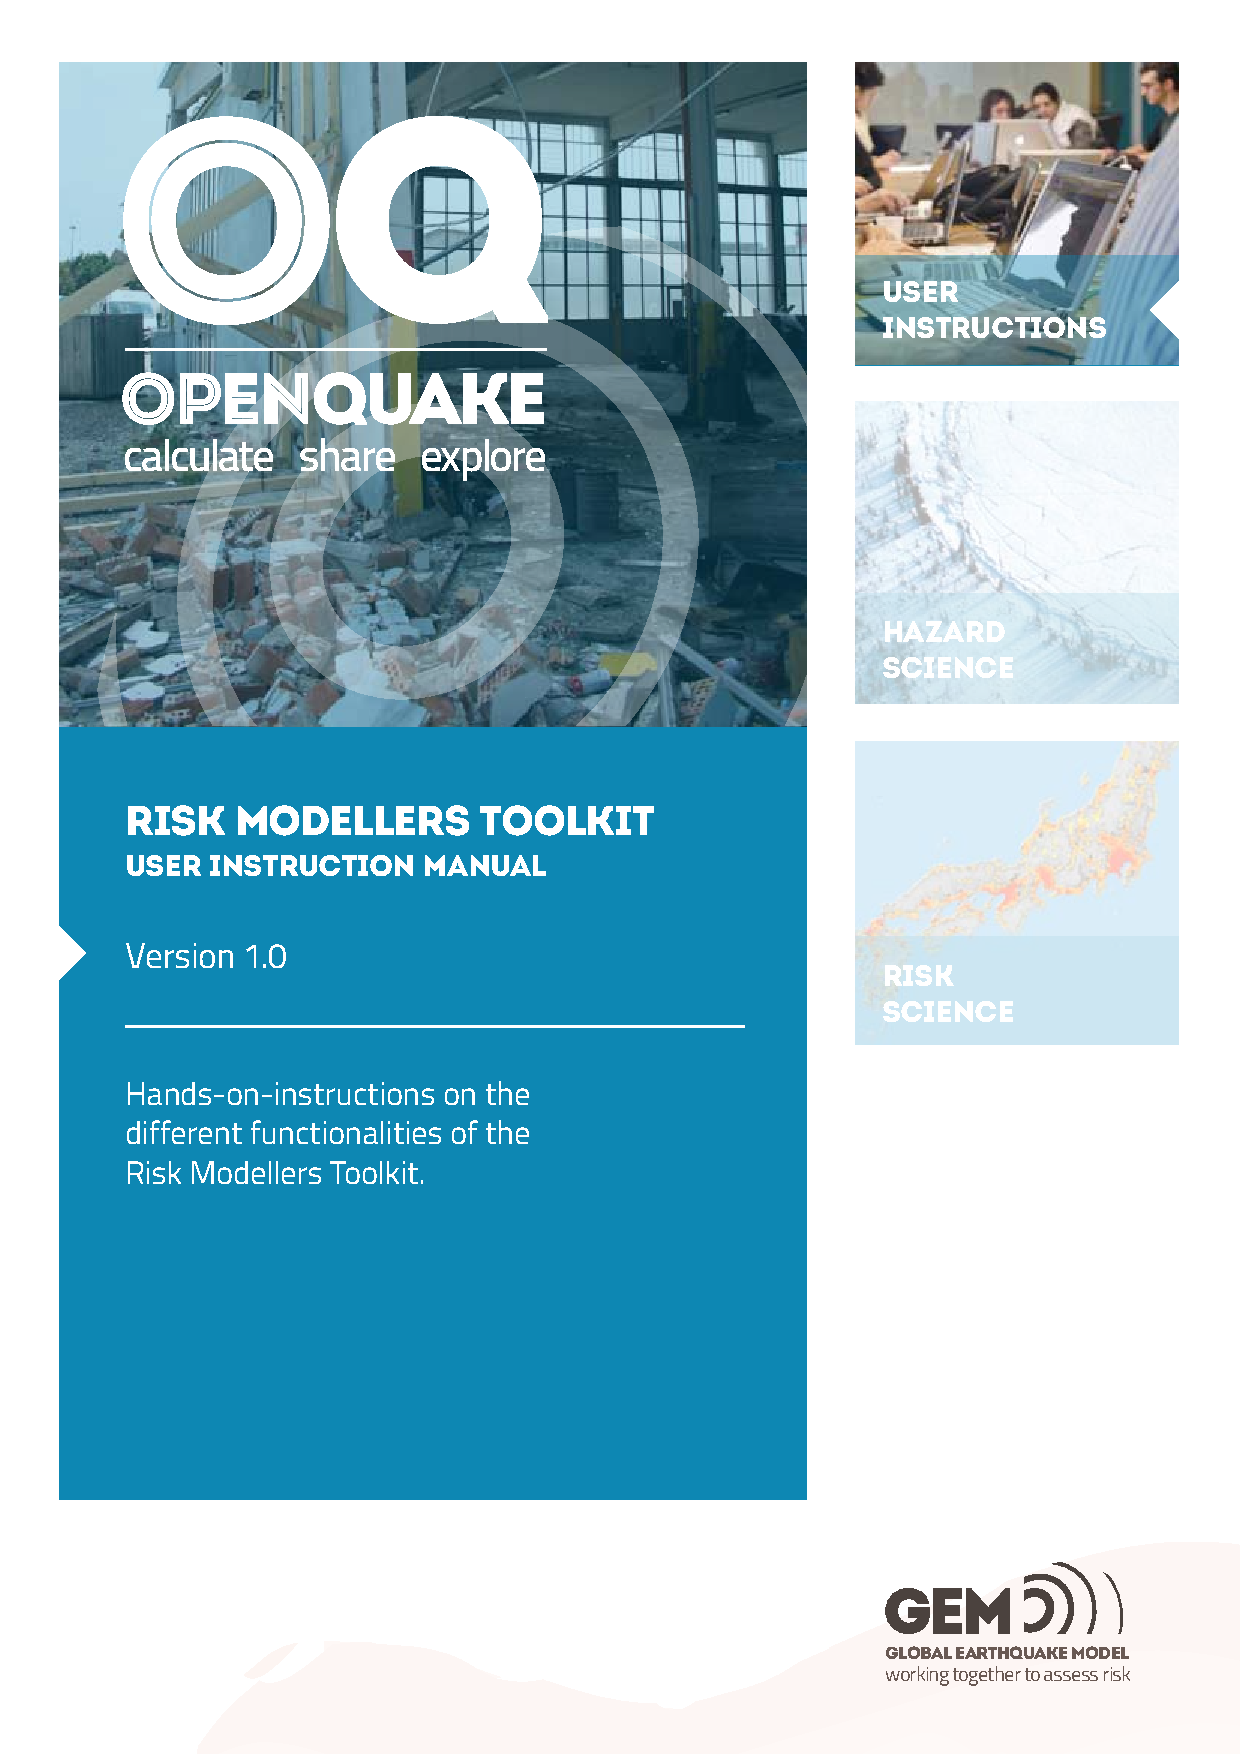
\includepdf[pages=-]{figures/rmtk-docs-cover.pdf}

%-------------------------------------------------------------------------------
%	TITLE PAGE
%-------------------------------------------------------------------------------

\begingroup
\thispagestyle{empty}
\begin{center}
\par\normalfont\fontsize{15}{15}\sffamily\selectfont
\textcolor{oqblue}{OpenQuake: calculate, share, explore}
\vspace*{9cm}
\par\bfseries\fontsize{35}{35}\sffamily\selectfont
\textcolor{gembrown}{Risk Modeller's Toolkit\\User Instruction Manual}\par
\vspace*{9cm}
\par\normalfont\fontsize{15}{15}\sffamily\selectfont
\href{https://github.com/GEMScienceTools/rmtk}{\textcolor{oqblue}{github.com/gemsciencetools/rmtk}}
\end{center}
\endgroup

%----------------------------------------------------------------------------------------
%	COPYRIGHT PAGE
%----------------------------------------------------------------------------------------

\newpage
\vfill
\thispagestyle{empty}

\noindent \copyright\ 2015 GEM Foundation\\ % Copyright notice

\noindent \textsc{Published by GEM Foundation}\\ % Publisher

\noindent \textsc{globalquakemodel.org/openquake}\\ % URL

\noindent
   {\textbf{Citation}} \hfill \\
   Please cite this document as:\\
   Silva, V., Casotto, C., Rao, A., Villar, M., Crowley, H. and Vamvatsikos, D. (2015) OpenQuake Risk Modeller's Toolkit - User Guide. 
   \textit{Global Earthquake Model (GEM). Technical Report 2015-09.\\ 
   doi: 10.13117/GEM.OPENQUAKE.MAN.RMTK.1.0/02, 97 pages.} \hfill \\

   {\bf{Disclaimer}} \hfill \\
\noindent
   The ``Risk Modeller's Tookit - User Guide'' is distributed in the hope 
   that it will be useful, but without any warranty: without 
   even the implied warranty of merchantability or fitness for a 
   particular purpose. While every 
   precaution has been taken in the preparation of this document, in 
   no event shall the authors of the manual and the GEM Foundation be 
   liable to any party for direct, indirect, special, incidental, or 
   consequential damages, including lost profits, arising out of the 
   use of information contained in this document or from the use of 
   programs and source code that may accompany it, even if the authors 
   and GEM Foundation have been advised of the possibility of such damage. 
   The Book provided hereunder is on as "as is" basis, and the authors 
   and GEM Foundation have no obligations to provide maintenance, support,
   updates, enhancements, or modifications. 
   \hfill \\
   The current version of the book has been revised only by members of 
   the GEM model facility and it must be considered a draft copy. 
   %
   \vspace{0.4cm} \hfill \\
   {\bf{License}} \hfill \\
   This Manual is distributed under the Creative Commons License 
   Attribution-NonCommercial-ShareAlike 4.0 International 
   (\href{http://creativecommons.org/licenses/by-nc-sa/4.0/}
   {CC BY-NC-SA 4.0}). 
   You can download this Manual and share it with 
   others as long as you provide proper credit, but you cannot change 
   it in any way or use it commercially.\hfill \\

\noindent \textit{First printing, September 2015} % Printing/edition date

%----------------------------------------------------------------------------------------
%	TABLE OF CONTENTS
%----------------------------------------------------------------------------------------

\chapterimage{figures/chapter_head_1.pdf} % Table of contents heading image
\pagestyle{empty} % No headers
\tableofcontents % Print the table of contents itself
\cleardoublepage % Forces the first chapter to start on an odd page so it's on the right
\pagestyle{fancy} % Print headers again

%----------------------------------------------------------------------------------------
%	PREAMBLE
%----------------------------------------------------------------------------------------
\chapterimage{figures/chapter_head_2.pdf} % Chapter heading image
\chapter*{Preface}
%\addcontentsline{toc}{chapter}{Preamble}
The goal of this book is to provide a comprehensive and transparent description
of the methodologies adopted and implemented in the Risk Modeller's Toolkit
(RMTK).
% Add short description about RMTK

% Add short description about main contributors
It is freely distributed under an Affero GPL license 
(more information available at this link 
\href{http://www.gnu.org/licenses/agpl-3.0.html}{http://www.gnu.org/licenses/agpl-3.0.html})

%----------------------------------------------------------------------------------------
%	CHAPTER 1
%----------------------------------------------------------------------------------------
% Introduction
\chapterimage{figures/chapter_head_2.pdf} % Chapter heading image
\chapter{Introduction}
\label{chap:introduction}
\section{Getting started}
The Risk Modeller's Toolkit makes extensive use of the Python programming language and the web-browser based interactive IPython notebook interface. As with OpenQuake, the preferred working environment is Ubuntu (12.04 or later) or Mac OS X. At present, the user  must install the dependencies manually. An effort has been made to keep the number of additional dependencies to a minimum. More information regarding the current dependencies of the toolkit can be found at \href{http://github.com/GEMScienceTools/rmtk}{http://github.com/GEMScienceTools/rmtk}.

The current dependencies are:
\begin{itemize}
\item Numpy and Scipy (included in the standard OpenQuake installation)
% \item OpenQuake RiskLib (included in the standard OpenQuake installation)
%     \hfill \\ (\href{http:/github.com/gem/oq-risklib}{http:/github.com/gem/oq-risklib})
\item Matplotlib (\href{http://matplotlib.org/}{http://matplotlib.org/})
\end{itemize}

The Matplotlib library can be installed easily from the command line by:

\begin{Verbatim}[frame=single, commandchars=\\\{\}, fontsize=\scriptsize]
~\$ sudo pip install matplotlib
\end{Verbatim}

To enable usage of the rmtk within any location in the operating system, OS X and Linux users should add the path to the rmtk folder to their profile file. This can be done as follows:

\begin{enumerate}
\item Using a command line text editor (e.g. VIM or Emacs), open the \verb=~/.profile= folder as follows:

\begin{Verbatim}[frame=single, commandchars=\\\{\}, fontsize=\scriptsize]
~\$ vim ~/.profile
\end{Verbatim}

\item At the bottom of the profile file (if one does not exist it will be created) add the line:

\begin{Verbatim}[frame=single, commandchars=\\\{\}, fontsize=\scriptsize]
export PYTHONPATH=/path/to/rmtk/folder/:\$PYTHONPATH
\end{Verbatim}

Where \verb=/path/to/rmtk/folder/= is the system path to the location of the rmtk folder (use the command \verb=pwd= from within the rmtk folder to view the full system path).

\item Reload the profile file using the command

\begin{Verbatim}[frame=single, commandchars=\\\{\}, fontsize=\scriptsize]
~\$ source ~/.profile
\end{Verbatim}

\end{enumerate}

The IPython Notebook is a browser-based notebook which provides support for interactive coding, text, mathematical expressions, inline plots and other rich media. Static notebooks can also be created for recording and distributing the results of the rich computations.

If you already have Python installed , you can get IPython along with the dependencies for the IPython notebook using pip:

\begin{Verbatim}[frame=single, commandchars=\\\{\}, samepage=true]
~\$ sudo pip install "ipython[notebook]"
\end{Verbatim}

A notebook session can be started via the command line:

\begin{Verbatim}[frame=single, commandchars=\\\{\}, samepage=true]
~\$ ipython notebook
\end{Verbatim}

This will print some information about the notebook server in your console, and open a web browser to the URL of the web application (by default, http://127.0.0.1:8888).

The landing page of the IPython notebook web application, the dashboard, shows the notebooks currently available in the notebook directory (by default, the directory from which the notebook server was started).

You can create new notebooks from the dashboard with the New Notebook button, or open existing ones by clicking on their name.

At present, the recommended approach for Windows users is to run Ubuntu Linux 12.04 within a Virtual Machine and install the rmtk following the instructions above. Up-to-date VirtualBox images containing the OpenQuake-engine and platform, and the Hazard and Risk Modeller's Toolkits are available here: \href{http://www.globalquakemodel.org/openquake/start/download/}{http://www.globalquakemodel.org/openquake/start/download/}

Knowledge of the Python programming language is not necessary in order to use the tools provided in the Risk Modeller's Toolkit. Nevertheless, a basic understanding of the data types and concepts of Python will come in handy if you are interested in modifying or enhancing the standard scripts provided in the toolkit. If you’ve never used Python before, the official \href{https://docs.python.org/2/tutorial/}{Python tutorial} is a good place to start. \href{http://www.swaroopch.com/notes/python/}{A Byte of Python} is also a well-written guide to Python and a great reference for beginners. Appendix \ref{sec:python_guide} at the end of this user manual also provides a quick-start guide to Python.

	\section{Current features}
	\label{sec:features}
	The Risk Modeller's Toolkit is currently divided into three modules:
\begin{description}
\item[Plotting tools:] The plotting module of the RMTK provides scripts and notebooks for visualising all of the different hazard and risk outputs produced by calculations performed using the OpenQuake-engine. The visualisation tools currently support plotting of seismic hazard curves, uniform hazard spectra, hazard maps, loss exceedance curves, probabilistic loss maps, and damage distribution statistics, amongst others. This module also allow users to convert the different results from the standard OpenQuake XML format into other formats such as CSV.
\item[Risk tools:] This module provides useful scripts to post-process OpenQuake hazard and risk results and calculate further metrics.
\item[Vulnerability tools:] This module implements several methodologies for estimating fragility and vulnerability functions for individual buildings or for a class of buildings. The provided scripts differ in level of complexity of the methodology and according to the type of input data available for the buildings under study. The guidelines for analytical vulnerability assessment provided by the GEM Global Vulnerability Consortium have been used as the primary reference for the development of this module.
\end{description}

A summary of the methods available in the present version is given in Table \ref{tab:current_features}.

\begin{table}[!htbp]
\centering
\begin{tabular}{|l|l|} \hline
\textbf{Module}     & \textbf{Feature / Methodology} \\ \hline
\textbf{Plotting}   & Hazard Curves \\
\textbf{Module}     & Uniform Hazard Spectra \\
                    & Hazard Maps \\
                    & Ground Motion Fields \\
                    & Collapse Maps \\
                    & Scenario Loss Maps \\
                    & Probabilistic Loss Maps \\
                    & Loss Curves \\
                    & Damage Distribution \\
                    & \\ \hline
\textbf{Risk}       & Probable Maximum Loss Calculator \\
\textbf{Module}     & Logic-Tree Branch Selector \\
                    & \\ \hline
\textbf{Vulnerability} & \textbf{Capacity Curve Generation} \\
\textbf{Module}        & DBELA \\
                    & SP-BELA \\
                    & Point Dispersion \\
                    & \\
                    & \textbf{MDOF$\to$SDOF Conversion} \\
                    & Single Mode of Vibration \\
                    & Adaptive Approach \\
                    & \\
                    & \textbf{Direct Nonlinear Static Methods} \\
                    & SPO2IDA \citep{VamvatsikosCornell2005} \\
                    & \citet{DolsekFajfar2004} \\
                    & \citet{RuizGarciaMiranda2007} \\
                    & \\
                    & \textbf{Record Based Nonlinear Static Methods} \\
                    & \citet{VidicEtAl1994} \\
                    & \citet{LinMiranda2008} \\
                    & \citet{Miranda2000} for Firm Soils \\
                    & N2 \citep{CEN2005} \\
                    & Capacity Spectrum Method \citep{FEMA4402005} \\
                    & DBELA \citep{SilvaEtAl2013} \\
                    & \\
                    & \textbf{Nonlinear Time History Analysis} \\
                    & for SDOF Oscillators \\ \hline
\end{tabular}
\caption{Current features in the OpenQuake Risk Modeller's Toolkit}
\label{tab:current_features}

\end{table}

	\section{Organization}
	\label{sec:organization}
	This manual is designed to explain the various functions in the toolkit, to provide the theoretical background behind them, and to guide the modeller in the use of the rmtk within the ``IPython Notebook'' environment. This novel tool implements Python inside a web-browser environment, permitting the user to execute real Python workflows, whilst allowing for images and text to be embedded. Its use is encouraged especially for beginner Python users for a more visual application of the rmtk.

The IPython Notebook  comes installed from version 1.0 of IPython, that can be installed from the Python package repository by entering:

\begin{Verbatim}[frame=single, commandchars=\\\{\}, samepage=true]
~\$ sudo pip install ipython
\end{Verbatim}

A notebook session can be started via the command:

\begin{Verbatim}[frame=single, commandchars=\\\{\}, samepage=true]
~\$ ipython notebook --pylab inline
\end{Verbatim}

The tutorial itself does not specifically require a working knowledge of Python. However, an understanding of the basic Python data types is highly desirable. Users who are new to Python are recommended to familiarise themselves with Appendix \ref{sec:python_guide} of this tutorial.

The \textit{rmtk} is currently subdivided into two classes of tools, the Vulnerability and Plotting tools, presented in Chapter 2 and Chapter 3 of this tutorial respectively. In the Vulnerability chapter the vulnerability methodologies implemented are classified in Non-linear Static (NLS) and Non-linear Dynamic (NLD) according to the structural analysis type performed to assess the response of the building. These two main sections (NLS and NLD) are organised as follows:

\begin{itemize}
\item General Introduction.
\item Getting Started, where it is explained what files need to be executed to start the vulnerability analysis, and what options are available to call the preferred methodology and to input the preferred data type.
\item Description of the methodologies.
\end{itemize}

Within the description of each methodology the user can find the following subsections:
\begin{itemize}
\item Theoretical description of the method.
\item Description and examples of the inputs.
\item Description of the workflow.
\end{itemize}

A summary of the algorithms available in the present version is given in Table \ref{tab:current_features}.
\begin{table}[!htbp]
\centering
\begin{tabular}{|c|c|} \hline
Feature & Algorithm\\ \hline
\textbf{Non-linear Static} & Cr-based (Ruiz-Garcia and Miranda, 2007)\\
    & Spo2ida (Vamvatsikos and Cornell, 2006) \\
    & R-$/mu$-T-based (Dolsek and Fajfar, 2004) \\ \hline
 \textbf{Non-linear Dynamic} & DPM-based (Silva et al. 2013)\\
  & Ida-postprocessing (Vamvatsikos and Cornell, 2002) \\ \hline
\end{tabular}
\caption{Current algorithms in the RMTK}
\label{tab:current_features}
\end{table}



%----------------------------------------------------------------------------------------
%	CHAPTER 2
%----------------------------------------------------------------------------------------
% Plotting part
\chapterimage{figures/chapter_head_2.pdf} % Chapter heading image
\chapter{Plotting}
\label{chap-plotting}
The OpenQuake-engine is capable of generating several seismic hazard and risk outputs, such as loss exceedance curves, seismic hazard curves, loss and hazard maps, damage statistics, amongst others. Most of these outputs are stored using the Natural Risk Markup Language (nrml), or simple comma separated value (csv) files. The Plotting module of the Risk Modellers Toolkit allows users to visualize the majority of the OpenQuake-engine results, as well as to convert them into other formats compatible with GIS software (e.g. QGIS). Despite the default styling of the maps and curves defined within the Risk Modellers Toolkit, it is important to state that any user can adjust the features of each output by modifying the original scripts.

	\section{Plotting damage distribution}
	\label{sec:plot-damage}
	Using the Scenario Damage Calculator \citep{SilvaEtAl2014a} of the OpenQuake-engine, it is possible to assess the distribution of damage for a collection of assets considering a single seismic event. These results include damage distributions per building typology, total damage distribution, and distribution of collapsed buildings in the region of interest.

\subsection{Plotting damage distributions}
\label{subsec:plot-damage_disag}
This feature of the Plotting module allows users to plot the distribution of damage across the various vulnerability classes, as well as the total damage distribution. For what concerns the former result, it is necessary to set the path to the output file using the parameter \verb=tax_dmg_dist_file=. It is also possible to specify which vulnerability classes should be considered, using the parameter \verb=taxonomy_list=. However, if a user wishes to consider all of the vulnerability classes, then this parameter should be left empty. It is also possible to specify if a 3D plot containing all of the vulnerability classes should be generated, or instead a 2D plot per vulnerability class. To follow the former option, the parameter \verb=plot_3d= should be set to \verb=True=. It is important to understand that this option leads to a plot of damage fractions for each vulnerability class, instead of the number of assets in each damage state. An example of this output is illustrated in Figure \ref{fig:damage_disag}.

\begin{figure}[htb]
  \centering
      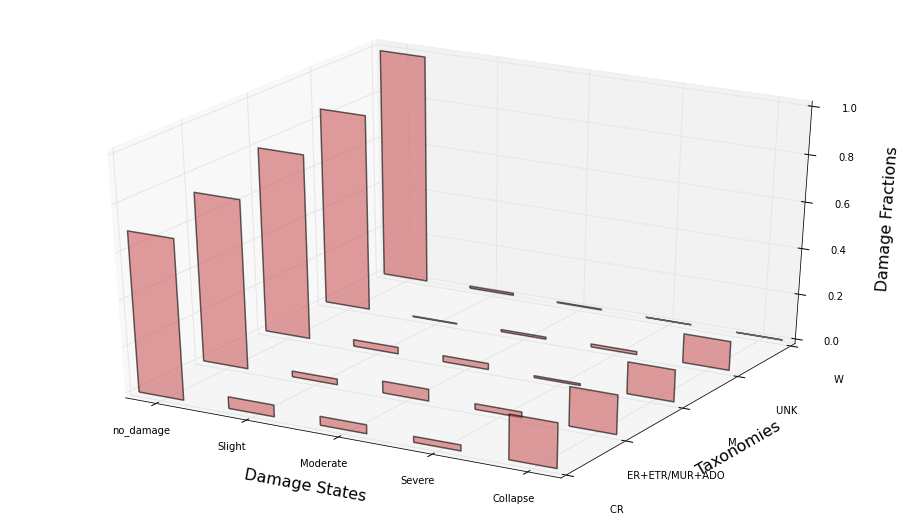
\includegraphics[width=10cm]{figures/damage_distribution.png}
  \caption{Damage distribution per vulnerability class.}
  \label{fig:damage_disag}
\end{figure}

In order to plot the total damage distribution (considering the entire collection of assets), it is necessary to use the parameter \verb=total_dmg_dist_file= to define the path to the respective output file. Figure \ref{fig:total_dmg} presents an example of this type of output.

\begin{figure}[htb]
  \centering
      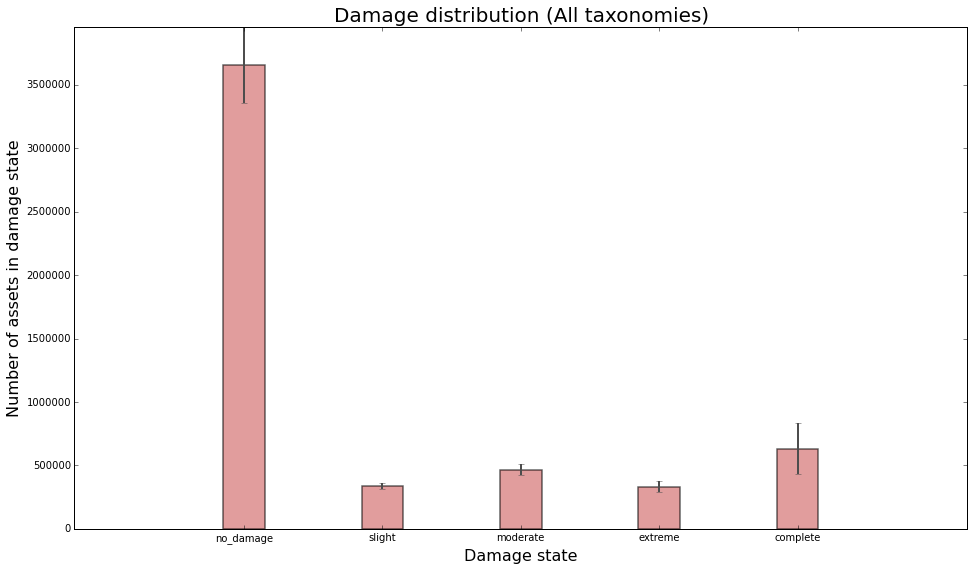
\includegraphics[width=8cm]{figures/total_damage_dist.png}
  \caption{Total damage distribution.}
  \label{fig:total_dmg}
\end{figure}

\subsection{Plotting collapse maps}
\label{subsec:plot-collapse_maps}

The OpenQuake-engine also generates an output defining the spatial distribution of the mean (and associated standard deviation) of assets in the last damage state (usually representing collapse or complete damage). The location of this output needs to be specified using the parameter \verb=collapse_map=. Then, it is necessary to specify whether the user desires a map with the aggregated number of collapsed assets (i.e. at each location, the mean number of collapsed assets across all of the vulnerability classes are summed) or a map for each vulnerability class. Thus, the following options are permitted:\\

\begin{enumerate}
\item Aggregated collapse map only.
\item Collapse maps per vulnerability class only.
\item Both aggregated and vulnerability class-based.\\
\end{enumerate}

The plotting option should be specified using the parameter \verb=plotting_type=, and the location of the exposure model used to perform the calculations must be defined using the variable \verb=exposure_model=. A number of other parameters can also be adjusted to modify the style of the resulting collapse map, as follows:\\

\begin{itemize}
\item \verb=bounding_box=: If set to 0, the Plotting module will calculate the geographical distribution of the assets, and adjust the limits of the map accordingly. Alternatively, a user can also specify the minimum / maximum latitude and longitude that should be used in the creation of the map.
\item \verb=marker_size=: This attribute can be used to adjust the size of the markers in the map.
\item \verb=log_scale=: If set to \verb=True=, it will apply a logarithmic scale on the colour scheme of the map, potentially allowing a better visualization of the variation of the numbers of collapsed assets in the region of interest.\\
\end{itemize}

An example of a collapse map is presented in Figure \ref{fig:collapse_map}.

\begin{figure}[htb]
  \centering
      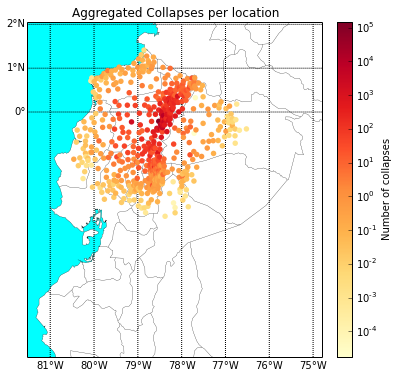
\includegraphics[width=8cm]{figures/collapse_map.png}
  \caption{Spatial distribution of the mean number of collapsed assets.}
  \label{fig:collapse_map}
\end{figure}

	
	\section{Plotting hazard and loss curves}
	\label{sec:plot-curves}
	Using the Classical PSHA-based or Probabilistic Event-based Calculators (\cite{SilvaEtAl2014a}, \cite{PaganiEtAl2014a}) of the OpenQuake-engine, it is possible to calculate seismic hazard curves for a number of locations, or loss exceedance curves considering a collection of spatially distributed assets.

\subsection{Plotting hazard curves and uniform hazard spectra}
\label{subsec:plot-hazard_curves}
A seismic hazard curve defines the probability of exceeding a number of intensity measure levels (e.g. peak ground acceleration or spectral acceleration) for a given interval of time (e.g. 50 years). In order to plot these curves, it is necessary to define the path to the output file in the parameter \verb=hazard_curve_file=. Then, since each output file might contained a great number of hazard curves, it is necessary to establish the location for each the hazard curve will be extracted. To visualize the list of locations comprised in the output file, the function \verb=hazard_curves.loc_list= can be employed. Then, the chosen location must be provided to the plotting function (e.g. \verb=hazard_curves.plot("81.213823|29.761172")=). An example of a seismic hazard curve is provided in Figure \ref{fig:hazard_curve}.\\

\begin{figure}[htb]
  \centering
      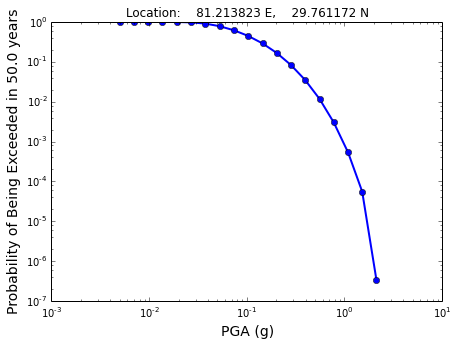
\includegraphics[width=9cm]{figures/hazard_curve.png}
  \caption{Seismic hazard curve for peak ground acceleration (PGA).}
  \label{fig:hazard_curve}
\end{figure}

To plot uniform hazard spectra (UHS), a similar approach should be followed. The output file containing the uniform hazard spectra should be defined using the parameter \verb=uhs_file=, and then a location must be provided to the plotting function (e.g.\verb=uhs.plot("81.213823|29.761172")=). An example of uniform hazard spectra is illustrated in Figure \ref{fig:UHS}.

\begin{figure}[htb]
  \centering
      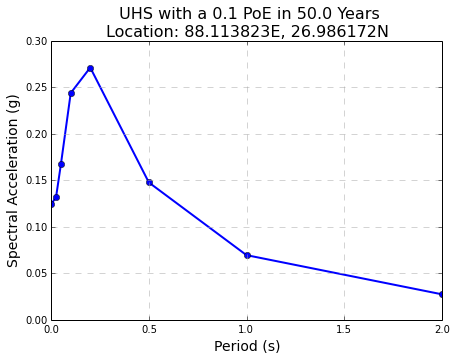
\includegraphics[width=9cm]{figures/UHS.png}
  \caption{Uniform Hazard Spectra for a probability of exceedance of 10\% in 50 years.}
  \label{fig:UHS}
\end{figure}

\subsection{Plotting loss curves}
\label{subsec:plot-loss_curves}
A loss exceedance curve defines the relation between a set of loss levels and the corresponding probability of exceedance within a given time span (e.g. a year). In order to plot these curves, it is necessary to define the location of the output file using the parameter \verb=loss_curves_file=. Since each output file may contains a large number of loss exceedance curves, it is necessary to define for which assets will the loss curves be extracted. The parameter \verb=assets_list= should be employed to define all of the chosen asset ids. These ids can be visualize directly on the loss curve output file, or on the exposure model used for the risk calculations. It is also possible to define a logarithmic scale for the x and y axis using the parameters \verb=log_scale_x= and \verb=log_scale_y=. A loss exceedance curve for a single asset is depicted in Figure \ref{fig:loss_curve}.

\begin{figure}[htb]
  \centering
      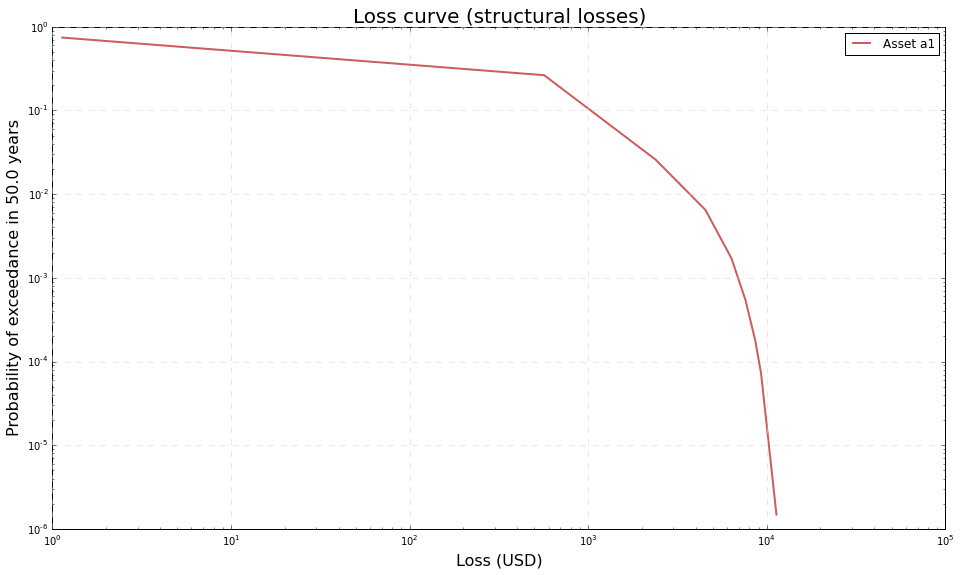
\includegraphics[width=8cm]{figures/loss_curve.png}
  \caption{Loss exceedance curve.}
  \label{fig:loss_curve}
\end{figure}
	
	\section{Plotting hazard and loss maps}
	\label{sec:plot-maps}
	The OpenQuake-engine offers the possibility of calculating seismic hazard and loss (or risk) maps. To do so, it utilizes the seismic hazard or loss exceedances curves, to estimate the corresponding hazard or loss for the pre-defined return period (or probability of exceedance within a given interval of time).

\subsection{Plotting hazard maps}
\label{subsec:plot-hazard_maps}
A seismic hazard map provides the expected ground motion (e.g. peak ground acceleration or spectral acceleration) at each location, for a certain return period (or probability of exceedance within a given interval of time). To plot this type of maps, it is necessary to specify the location of the output file using the parameter \verb=hazard_map_file=. An example hazard map is displayed in Figure \ref{fig:hazard_curve}.

\begin{figure}[htb]
  \centering
      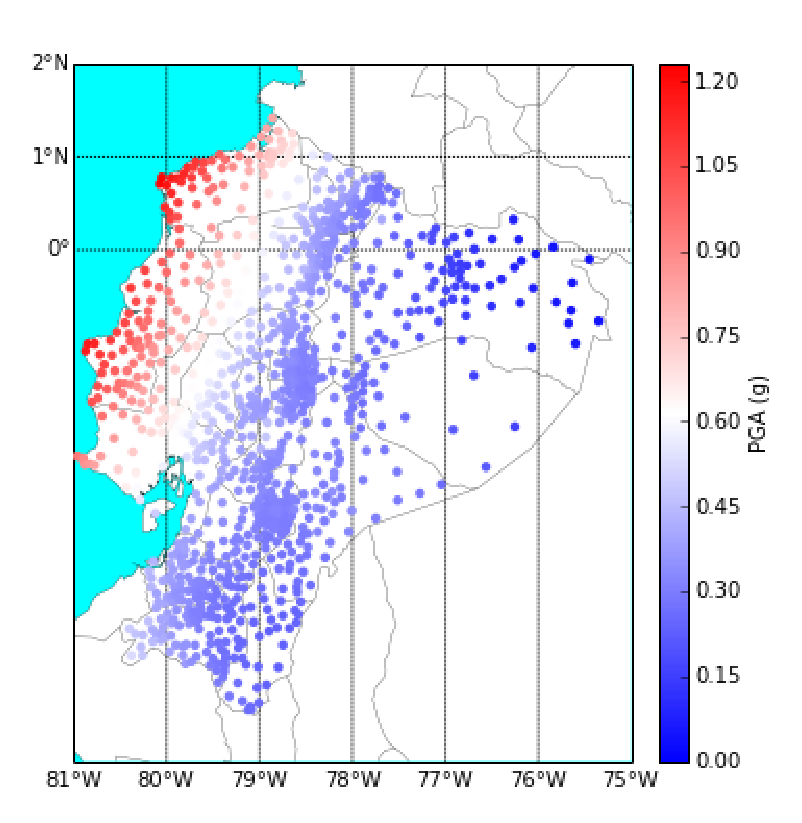
\includegraphics[width=7cm]{figures/hazard_Ecuador.eps}
  \caption{Seismic hazard map for a probability of exceedance of 10\% in 50 years.}
  \label{fig:hazard_map}
\end{figure}

\subsection{Plotting loss maps}
\label{subsec:plot-loss_maps}
A loss map provides the estimated losses for a collection of assets, for a certain return period (or probability of exceedance within a given interval of time). It is important to understand that these maps are not providing the distribution of losses for a seismic event for the chosen return period, nor the losses whose sum would correspond to the aggreagted loss for the same return period. This type of maps is simply providing the expected loss for a specified level of frequency for each asset. 
To use this feature, it is necessary to define the parth ot the output file using the parameter \verb=loss_map_file=, as well as the exposure model used to perform the risk calculations through the parameter \verb=exposure_model=. Then, similarly to what was explained in section \ref{subsec:plot-collapse_maps} for collapse maps, it is possible to follow three approaches to generate the loss maps:\\ 

\begin{enumerate}
\item Aggregated loss map only.
\item Loss maps per taxonomy only.
\item Both aggregated and taxonomy-based.\\
\end{enumerate}

Then, there are a number of options that can be used to modify the style of the maps. These include the size of the marker of the map (\verb=marker_size=), the geographical limits of the map (\verb=bounding_box=), and the employment of a logarithmic spacing for the color scheme (\verb=log_scale=). An example loss map for a single vulnerability class is presented in Figure \ref{fig:loss_map}.

\begin{figure}[htb]
  \centering
      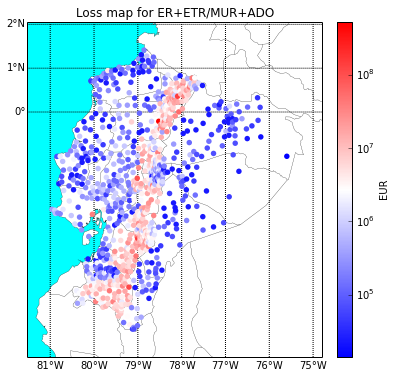
\includegraphics[width=7cm]{figures/loss_map.png}
  \caption{Loss (economic) map for a probability of exceedance of 10\% in 50 years.}
  \label{fig:loss_map}
\end{figure}

As mentioned on the introductory section, it is also possible to convert any of the maps into a format (csv) easily readable by GIS software. To do so, it is necessary to set the parameter \verb=export_map_to_csv= to \verb=True=. As an example, a map containing the average annual losses for Ecuador has been converted to the \verb=csv= format, and introduced into the QGIS software to produce the map presented in Figure \ref{fig:all_loss_map}.

\begin{figure}[htb]
  \centering
      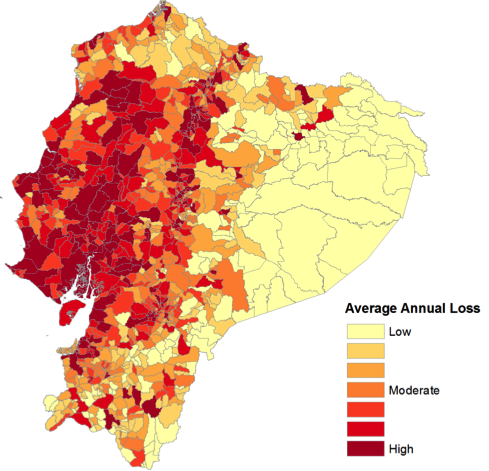
\includegraphics[width=6cm]{figures/loss_map_AAL.png}
  \caption{Average annual (economic) losses for Ecuador.}
  \label{fig:all_loss_map}
\end{figure}


%----------------------------------------------------------------------------------------
%	CHAPTER 3
%----------------------------------------------------------------------------------------
% Risk part
\chapterimage{figures/chapter_head_2.pdf} % Chapter heading image
\chapter{Risk}
\label{chap:risk}
The OpenQuake-engine currently generates the most commonly used seismic hazard and risk results (e.g. hazard maps, loss curves, average annual losses). However, it is recognized that there are a number of other risk metrics that might not be of interest of the general GEM community, but fundamental for specific users. This module of the Risk Modeller's Toolkit aims to provide users with additional risk results and functionalities, based on the standard output of the OpenQuake-engine.

	\section{Deriving Probable Maximum Losses (PML)}
	\label{sec:derive-pml}
	The Probabilistic Event-based Risk calculator (\citep{SilvaEtAl2014a}) of the OpenQuake-engine is capable of calculating event loss tables, which contain a list of earthquake ruptures and associarted losses. These losses my refer to specific assets, or the sum of the losses from the entire building portfolio (aggregated loss curves). 
Using this module, it is possible to derive a probable maximum loss (PML) curves (i.e. relation between a set of loss levels and corresponding return peridos of exceedance), as illustrated in Figure \ref{fig:pml}.

\begin{figure}[htb]
  \centering
      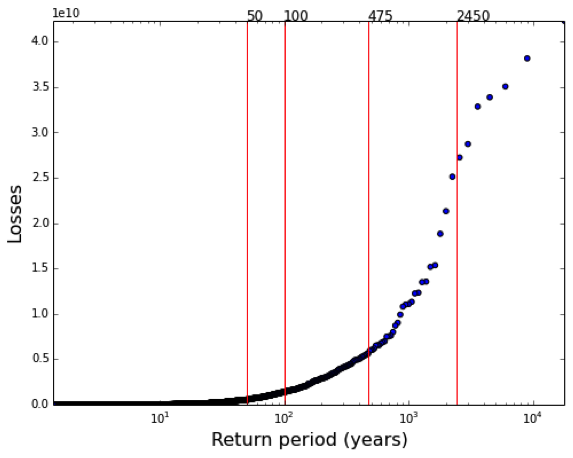
\includegraphics[width=8cm]{figures/pml_example.png}
  \caption{Probable Maximum Loss (PML) curve.}
  \label{fig:pml}
\end{figure}

To use this feature, it is necessary to use the parameter \verb=event_loss_table_folder= to specify the location of the folder that contains the set of event loss tables and stochastic event sets. Then, it is also necessary to provide the total economic value of the building portfolio (using the variable \verb=total_cost=) and the list of return periods of interest (using the variable \verb=return_periods=). This module also offers the possibility of saving all of the information in \verb=csv= files, which can be used in other software (e.g. Microsoft Excel) for other purposes. To do so, the parameters \verb=save_elt_csv= and \verb=save_ses_csv= should be set to \verb=True=.

	\section{Selecting a logic tree branch}
	\label{sec:logic-tree}
	When a non-trivial logic-tree is used to capture the model uncertainty in the source model or in the choice of an appropriate ground motion prediction equation (GMPE) for each of the tectonic region types in the region considered, OpenQuake can calculate the hazard curves for each end-branch of the logic-tree individually. Now, if a risk modeller wishes to estimate damage or losses using one or a few of these branches only, it is useful to compare the hazard curves for the chosen branch with the mean hazard curve. Depending upon the distance of the hazard curve for a particular branch from the mean hazard curve, the risk modeller may wish to choose the branches for which the hazard curves are closest to the mean hazard curve. This Python script and corresponding IPython notebook allow the risk modeller to list the end-branches for the hazard calculation, sorted in increasing order of the distance of the branch hazard curve from the mean hazard curve. Currently, the distance metric used for performing the sorting is the root mean square distance.

%----------------------------------------------------------------------------------------
%	CHAPTER 4
%----------------------------------------------------------------------------------------
% Vulnerability part
\chapterimage{figures/chapter_head_2.pdf} % Chapter heading image
\chapter{Vulnerability}
\label{chap:vulnerability}

    \section{Introduction}
    Seismic fragility and vulnerability functions form an integral part of a seismic risk assessment project, along with the seismic hazard and exposure models. Fragility functions for a building or a class of buildings are typically associated with a set of discrete damage states. A fragility function defines the probabilities of exceedance for each of these damage states as a function of the intensity of ground motion. A vulnerability function for a building or a class of buildings defines the probability of exceedance of loss values as a function of the intensity of ground motion. A consequence model, sometimes also referred to as a damage-to-loss model, which describes the expected loss for different damage states, can be used to derive the vulnerability function for a building or a class of buildings from the corresponding fragility function.

Empirical methods are often preferred for the derivation of fragility and vulnerability functions when relevant data regarding the levels of physical damage and loss at various levels of ground shaking are available from past earthquakes. However, the major drawback of empirical methods is the highly limited quantity and quality of damage and repair cost data and the corresponding ground shaking intensities available from previous events.

The analytical approach to derive fragility and vulnerability functions for an individual structure relies on creating a numerical model of the structure and assessing the deformation behaviour of the modelled structure by subjecting it to selected ground motion acceleration records or predetermined lateral load patterns. The deformation then needs to be related to physical damage to obtain the fragility functions. The fragility functions can be combined with the appropriate consequence model to derive the vulnerability function for the structure. Fragility and vulnerability functions for a class of buildings (a "building typology") can be obtained by considering a number of structures considered representative of that class. A combination of Monte Carlo sampling followed by regression analysis can be used to obtain a single "representative" fragility or vulnerability function for the building typology.

The level of sophistication employed during the structural analysis stage is constrained both by the amount of time and the types of information regarding the structure available to the modeller. Although performing nonlinear dynamic analysis of a highly detailed model of the structure using several accelerograms is likely to yield a more representative picture of the dynamic deformation behaviour of the real structure during earthquakes, nonlinear static analysis is often preferred due to the lower modelling complexity and computational effort demanded by static methods. Different researchers have proposed different methodologies to derive fragility functions using pushover or capacity curves from nonlinear static analyses. Several of these methodologies have already been implemented in the RMTK. The following sections of this chapter describe some of these techniques in more detail.

    \section{Definition of input models}
    \section{Getting started}
The Risk Modeller's Toolkit makes extensive use of the Python programming language and the web-browser based interactive IPython notebook interface. As with OpenQuake, the preferred working environment is Ubuntu (12.04 or later) or Mac OS X. At present, the user  must install the dependencies manually. An effort has been made to keep the number of additional dependencies to a minimum. More information regarding the current dependencies of the toolkit can be found at \href{http://github.com/GEMScienceTools/rmtk}{http://github.com/GEMScienceTools/rmtk}.

The current dependencies are:
\begin{itemize}
\item Numpy and Scipy (included in the standard OpenQuake installation)
% \item OpenQuake RiskLib (included in the standard OpenQuake installation)
%     \hfill \\ (\href{http:/github.com/gem/oq-risklib}{http:/github.com/gem/oq-risklib})
\item Matplotlib (\href{http://matplotlib.org/}{http://matplotlib.org/})
\end{itemize}

The Matplotlib library can be installed easily from the command line by:

\begin{Verbatim}[frame=single, commandchars=\\\{\}, fontsize=\scriptsize]
~\$ sudo pip install matplotlib
\end{Verbatim}

To enable usage of the rmtk within any location in the operating system, OS X and Linux users should add the path to the rmtk folder to their profile file. This can be done as follows:

\begin{enumerate}
\item Using a command line text editor (e.g. VIM or Emacs), open the \verb=~/.profile= folder as follows:

\begin{Verbatim}[frame=single, commandchars=\\\{\}, fontsize=\scriptsize]
~\$ vim ~/.profile
\end{Verbatim}

\item At the bottom of the profile file (if one does not exist it will be created) add the line:

\begin{Verbatim}[frame=single, commandchars=\\\{\}, fontsize=\scriptsize]
export PYTHONPATH=/path/to/rmtk/folder/:\$PYTHONPATH
\end{Verbatim}

Where \verb=/path/to/rmtk/folder/= is the system path to the location of the rmtk folder (use the command \verb=pwd= from within the rmtk folder to view the full system path).

\item Reload the profile file using the command

\begin{Verbatim}[frame=single, commandchars=\\\{\}, fontsize=\scriptsize]
~\$ source ~/.profile
\end{Verbatim}

\end{enumerate}

The IPython Notebook is a browser-based notebook which provides support for interactive coding, text, mathematical expressions, inline plots and other rich media. Static notebooks can also be created for recording and distributing the results of the rich computations.

If you already have Python installed , you can get IPython along with the dependencies for the IPython notebook using pip:

\begin{Verbatim}[frame=single, commandchars=\\\{\}, samepage=true]
~\$ sudo pip install "ipython[notebook]"
\end{Verbatim}

A notebook session can be started via the command line:

\begin{Verbatim}[frame=single, commandchars=\\\{\}, samepage=true]
~\$ ipython notebook
\end{Verbatim}

This will print some information about the notebook server in your console, and open a web browser to the URL of the web application (by default, http://127.0.0.1:8888).

The landing page of the IPython notebook web application, the dashboard, shows the notebooks currently available in the notebook directory (by default, the directory from which the notebook server was started).

You can create new notebooks from the dashboard with the New Notebook button, or open existing ones by clicking on their name.

At present, the recommended approach for Windows users is to run Ubuntu Linux 12.04 within a Virtual Machine and install the rmtk following the instructions above. Up-to-date VirtualBox images containing the OpenQuake-engine and platform, and the Hazard and Risk Modeller's Toolkits are available here: \href{http://www.globalquakemodel.org/openquake/start/download/}{http://www.globalquakemodel.org/openquake/start/download/}

Knowledge of the Python programming language is not necessary in order to use the tools provided in the Risk Modeller's Toolkit. Nevertheless, a basic understanding of the data types and concepts of Python will come in handy if you are interested in modifying or enhancing the standard scripts provided in the toolkit. If you’ve never used Python before, the official \href{https://docs.python.org/2/tutorial/}{Python tutorial} is a good place to start. \href{http://www.swaroopch.com/notes/python/}{A Byte of Python} is also a well-written guide to Python and a great reference for beginners. Appendix \ref{sec:python_guide} at the end of this user manual also provides a quick-start guide to Python.

		\subsection{Definition of capacity curves}
		\label{subsec:cap_curves}
		The derivation of fragility models requires the description of the characteristics of the system to be assessed. A full characterisation of a structure can be done with an analytical structural model, but for the use in some fragility methodologies its fundamental features can be adequately described using a pushover curve, which describes the nonlinear behaviour of each input structure subjected to a horizontal lateral load.

Different methodologies require the pushover curve to be expressed with different parameters and to be combined with additional building information (e.g. period of the structure, height of the structure). The following input models have thus been implemented in the Risk Modeller's Toolkit:\\

\begin{enumerate}
 \item \verb=Base Shear vs Roof Displacement=
 \item \verb=Base Shear vs Floor Displacements=
 \item \verb=Spectral acceleration vs Spectral displacement=\\
\end{enumerate}

Within the description of each fragility methodology provided below, the required input model and the additional building information are specified. Moreover some methodologies give the user the chance to select the input model that fits better to the data at his or her disposal. Considering that different methodologies sharing the same input model may need different parameters, not all the information defined in the input file are necessarily used by each method. The various inputs are currently being stored in a \verb=csv= file (tabular format), as illustrated in the following Sections for each input model.

Once the pushover curves have been defined in the input file and uploaded in the IPython notebook, they can be visualised with the following function:

\begin{Verbatim}[frame=single, commandchars=\\\{\}, samepage=true]
utils.plot_capacity_curves(capacity_curves)
\end{Verbatim}


\subsubsection{Base Shear vs Roof Displacement}
\label{subsubsec:VB-Droof}
Some methodologies require the pushover curve to be expressed in terms of Base Shear vs Roof Displacement (e.g. Dolsek and Fajfar 2004 in Section~\ref{subsec:DolsekFajfar}, SPO2IDA in Section~\ref{subsec:SPO2IDA}). Additional building information is needed to convert the pushover curve (referring to a Multi Degree of Freedom, MDoF, system) to a capacity curve (Single Degree of Freedom, SDoF, system).\\

When the pushover curve is expressed in terms of Base Shear vs Roof Displacement, the user has to set the \verb=Vb-droof= variable to \verb=TRUE= in the input file, and define whether it is an idealised (e.g. bilinear) or a full pushover curve (i.e. with many pairs of base shear and roof displacement values), setting the variable \verb=Idealised= to \verb=TRUE= or \verb=FALSE= respectively. Then the following information about the structures to be assessed is needed:\\

\begin{enumerate}
\item \verb=Periods=, first period of vibration T$_1$.
\item \verb=Ground height=, height of the ground floor.
\item \verb=Regular height=, height of the regular floors.
\item \verb=Gamma participation factors=, modal participation factor $\Gamma_1$ of the first mode of vibration, normalised with respect to the roof displacement.
\item \verb=Effective modal masses=, effective modal masses $M_{1}^{*}$ of the first mode of vibration, normalised with respect to the roof displacement (see Section \ref{subsec:one_mode} for description).
\item \verb=Number storeys=, number of storeys.
\item \verb=Weight=, weight assigned to each structure for the derivation of fragility models for many buildings.
\item \verb=Vbn=, the base shear vector of the n$^{th}$ structure.
\item \verb=droofn=, the roof displacement vector of the n$^{th}$ structure. \\
\end{enumerate}

Only bilinear and quadrilinear idealisation shapes are currently supported to express the pushover curve in an idealised format, therefore the $V_b$ and $d_{roof}$ vectors should contain 3 or 5 $V_b$-$d_{roof}$ pairs, respectively, as described in the following lists and illustrated in Figures \ref{fig:bilinear} and \ref{fig:quadrilinear}.\\

Bilinear idealisation inputs:
\begin{itemize}
\item Displacement vector: displacement at Vb = 0 ($d_0$), yielding displacement ($d_1$), ultimate displacement ($d_2$).
\item Base Shear vector: Vb = 0, base shear at yielding displacement ($Vb_1$), base shear at ultimate displacement ($Vb_2$ = $Vb_1$).\\
\end{itemize}
\begin{figure}[htb]
  \centering
      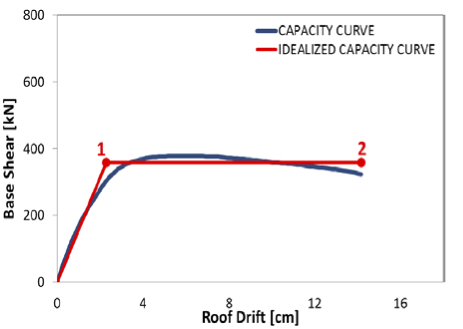
\includegraphics[width=9cm]{figures/bilinear.jpg}
  \caption{Inputs for bilinear idealisation of pushover curve.}
  \label{fig:bilinear}
\end{figure}

Quadrilinear idealisation inputs:
\begin{itemize}
\item Displacement vector: displacement at Vb = 0 ($d_0$), yielding displacement ($d_1$), displacement at maximum base shear ($d_2$), displacement at onset of residual force plateau ($d_3$), ultimate displacement ($d_4$).
\item Base Shear vector: Vb = 0, base shear at yielding displacement ($Vb_1$), maximum base shear ($Vb_2$), residual force ($Vb_3$) and force at ultimate displacement ($Vb_4$).\\
\end{itemize} 

\begin{figure}[htb]
  \centering
      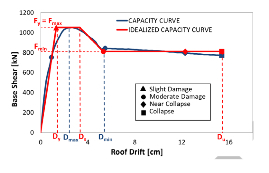
\includegraphics[width=9cm]{figures/quadrilinear.jpg}
  \caption{Inputs for quadrilinear idealisation of pushover curve.}
  \label{fig:quadrilinear}
\end{figure}

An example of an input \verb=csv= file for the derivation of a fragility model for a set of two structures, whose pushover curves are expressed with an idealised bilinear shape, is presented in Table \ref{table:Vb-droof_input}.

\begin {table}[htb]
\caption{Example of a Base Shear-Roof Displacement input model.}
\label{table:Vb-droof_input}
\begin{center}
  \begin{tabular}{ | c | c | c | c | c |}
  \hline
    Vb-droof & TRUE &  &  \\ \hline
    Vb-dfloor & FALSE & & \\ \hline
    Sd-Sa & FALSE & & \\ \hline
    Idealised & TRUE & & \\ \hline
    Periods [s] & 1.61 & 1.5 & \\ \hline
    Ground heights [m] & 7 & 6.5 & \\ \hline
    Regular heights [m] & 2.7 & 3.0 & \\ \hline
    Gamma participation factors & 1.29 & 1.4 & \\ \hline
    Effective modal masses & 232 &	230 &  \\ \hline
    Number storeys & 6 & 6 & \\ \hline
    Weights & 0.5 & 0.5 & \\ \hline
    Vb1 [kN] & 0 & 2090 & 2090 \\ \hline
    droof1 [m] & 0 & 0.1 & 0.6 \\ \hline
    Vb2 [kN] & 0 & 1700 & 1700 \\ \hline
    droof2 [m] & 0 & 0.08 & 0.5 \\ \hline
  \end{tabular}
\end{center}
\end{table}

Base shear vs Roof Displacement pushover curves can be idealised with bilinear and quadrilinear formats, according to \citep{FEMA4402005} and to the GEM Vulnerability guidelines (\citep{Dayala2014}), respectively, using the following function:

\begin{Verbatim}[frame=single, commandchars=\\\{\}, samepage=true]
idealised_capacity = utils.idealisation(idealised_type, capacity_curves)
\end{Verbatim}

\subsubsection{Base Shear vs Floor Displacements}
\label{subsubsec:VB-Dfloor}
A modification of the previous input model is the Base Shear vs Floor Displacements input type. In this case the conversion to a SDoF capacity curve is still based on the roof displacement, but a mapping scheme between the roof displacement and inter-storey drift at each floor level is also derived, so that the overall deformation state of the structure corresponding to a given roof displacement can be checked.\\
When the pushover curve is expressed in terms of Base Shear vs Floor Displacements, the user has to set the \verb=Vb-floor= variable to \verb=TRUE= in the input file. Only full pushover curves can be input, therefore the variable \verb=Idealised= should be set to \verb=FALSE=. Then the following information about the structures to be assessed is needed:\\

\begin{enumerate}
\item \verb=Periods=, first period of vibration T$_1$.
\item \verb=Ground height=, height of the ground floor.
\item \verb=Regular height=, height of the regular floors.
\item \verb=Gamma participation factors=, modal participation factor $\Gamma_1$ of the first mode of vibration, normalised with respect to the roof displacement.
\item \verb=Effective modal masses=, effective modal masses $M_{1}^{*}$ of the first mode of vibration, normalised with respect to the roof displacement (see Section \ref{subsec:one_mode} for description).
\item \verb=Number storeys=, number of storeys.
\item \verb=Weight=, weight assigned to each structure for the derivation of fragility models for many buildings.
\item \verb=Vbn=, the base shear vector of the n$^{th}$ structure.
\item \verb=dfloorn-1=, the displacement vector of the 1$^{st}$ floor of the n$^{th}$ structure.
\item \verb=dfloorn-2=, the displacement vector of the 2$^{nd}$ floor of the n$^{th}$ structure.
\item \verb=dfloorn-k=, the displacement vector of the k$^{th}$ floor of the n$^{th}$ structure. \\
\end{enumerate}

An example of an input \verb=csv= file for the derivation of a fragility model for a set of two structures, is presented in Table~\ref{table:Vb-dfloor_input}.

\begin {table}[htb]
\caption{Example of a Base Shear-Floor Displacements input model.}
\label{table:Vb-dfloor_input}
\begin{center}
  \begin{tabular}{ | c | c | c | c | c | c | c | c |}
  \hline
    Vb-droof & TRUE &  &  & & & \\ \hline
    Vb-dfloor & FALSE & & & & &  \\ \hline
    Sd-Sa & FALSE & & & & & \\ \hline
    Idealised & FALSE & & & & & \\ \hline
    Periods [s] & 1.61 & 1.5 & & & & \\ \hline
    Ground heights [m] & 7 & 6.5 & & & & \\ \hline
    Regular heights [m] & 2.7 & 3.0 & & & & \\ \hline
    Gamma participation factors & 1.29 & 1.4 & & & & \\ \hline
    Effective modal masses	& 232 &	230 & & & & \\ \hline
    Number storeys & 6 & 6 & & & & \\ \hline
    Weights & 0.5 & 0.5 & & & & \\ \hline
    Vb1 [kN] & 0	& ...	& 50	& 94	& 118	& \\ \hline
	  dfloor1-1 [m] & 0.002	& ...	& 0.05	& 0.09	& 0.11	& \\ \hline
	  dfloor1-2 [m] & 0.004	& ...	& 0.12	& 0.16	& 0.20	& \\ \hline
    Vb2 [kN] & 0	& ...	& 79	& 100	& 105	& 150 \\ \hline
    dfloor2-1 [m] & 0.006 &	...	& 0.018	& 0.023	& 0.05	& 0.1 \\ \hline
	dfloor2-2 [m] & 0.008	& ... &	0.023	& 0.030	& 0.038	& 0.15 \\ \hline
  \end{tabular}
\end{center}
\end{table}

Base shear vs Floor Displacement pushover curves can be idealised with bilinear and quadrilinear formats, according to \citep{FEMA4402005} and to the GEM Vulnerability guidelines (\citep{Dayala2014}), respectively, using the following function:

\begin{Verbatim}[frame=single, commandchars=\\\{\}, samepage=true]
idealised_capacity = utils.idealisation(idealised_type, capacity_curves)
\end{Verbatim}

\subsubsection{Spectral acceleration vs Spectral displacement}
\label{subsubsec:Sa-Sd}
Some methodologies work directly with capacity-curves (Spectral acceleration vs Spectral displacement) of SDoF systems (e.g. N2 in Section~\ref{subsec:N2}, CSM in Section~\ref{subsec:CSM}), so that the user can provide his or her own conversion of pushover curves, or can use the "Conversion from MDOF to SDOF" module in Section~\ref{sec:mdof_to_sdof}.\\
When the pushover curve is expressed in terms of Spectral acceleration vs Spectral displacement, the user has to set the \verb=Sd-Sa= variable to \verb=TRUE= in the input file. Then the following information about the structures to be assessed is needed:\\

\begin{enumerate}
\item \verb=Periods=, first periods of vibration T$_1$.
\item \verb=Heights=, heights of the structure.
\item \verb=Gamma participation factors=, modal participation factors $\Gamma_1$ of the first mode of vibration.
\item \verb=Effective modal masses=, effective modal masses $M_{1}^{*}$ of the first mode of vibration, normalised with respect to the roof displacement (see Section \ref{subsec:one_mode} for description).
\item \verb=Sdy=, the yielding spectral displacements.
\item \verb=Say=, the yielding spectral accelerations.
\item \verb=Sdn [m]=, the Sd vector of the n$^{th}$ structure.
\item \verb=San [g]=, the Sa vector of the n$^{th}$ structure. \\
\end{enumerate}

An example of an input \verb=csv= file for the derivation of a fragility model for a set of three structures, is presented in Table \ref{table:Sa-Sd_input}.

\begin {table}[htb]
\caption{Example of a Spectral acceleration-Spectral displacement input model.}
\label{table:Sa-Sd_input}
\begin{center}
  \begin{tabular}{ | c | c | c | c | c |}
  \hline
	Vb-droof &	FALSE & &  \\ \hline
	Vb-dfloor & 	FALSE & & \\ \hline
	Sd-Sa &	TRUE & & \\ \hline
	Periods [s] &	1.52 &	1.63 &	1.25 \\ \hline
	Heights [m]	& 6 &	6	& 6 \\ \hline
	Gamma participation factors	& 1.24 &	1.22 &	1.27 \\ \hline
	Effective modal masses	& 232 &	230 &	240 \\ \hline
	Sdy [m] & 	0.0821 & 	0.0972 &	0.0533\\ \hline
	Say [g]	& 0.143	& 0.14723	& 0.13728 \\ \hline
	Sd1 [m]	& 0 &	0.0821	& 0.238 \\ \hline
	Sa1 [g]	& 0	& 0.143	& 0.143 \\ \hline
	Sd2 [m] &	0 & 0.0972	& 0.264 \\ \hline
	Sa2 [g]	& 0	& 0.14723	& 0.14723 \\ \hline
	Sd3 [m]	& 0	& 0.0533	& 0.0964 \\ \hline
	Sa3 [g]	& 0	& 0.13728	& 0.13728 \\ \hline
  \end{tabular}
\end{center}
\end{table}

Capacity curves can be idealised with bilinear and quadrilinear formats, according to \citep{FEMA4402005} and to the GEM Vulnerability guidelines (\citep{Dayala2014}), respectively, using the following function:

\begin{Verbatim}[frame=single, commandchars=\\\{\}, samepage=true]
idealised_capacity = utils.idealisation(idealised_type, capacity_curves)
\end{Verbatim}

		\subsection{Definition of ground motion records}
		\label{subsec:gmrs}
		The record-to-record variability is one of the most important sources of uncertainty in fragility assessment. In the Direct Nonlinear Static Procedures implemented in the Risk Modellers Toolkit (see Section~\ref{subsec:direct-nsp}), this source of uncertainty is directly introduce in the fragility estimates, based on previous nonlinear analyses. In the Record-based Nonlinear Static Procedures (Section~\ref{subsec:record-nsp}) or in the Nonlinear Time History Analysis in Single Degree of Freedom Oscilators (Section~\ref{subsec:NLTHA_SDOF}), users have the possibility of introducing their own ground motion records. Each accelerogram needs to be stored in a \verb=csv= file (tabular format), as depicted in Table~\ref{table:gmr}. This file format uses two columns, in which the first one contains the time (in seconds) and the second the corresponding acceleration (in g).\\

\begin {table}[htb]
\caption{Example of a ground motion record.}
\label{table:gmr}
\begin{center}
  \begin{tabular}{ | c | c |}
  \hline
0.01 & 0.0211 \\ \hline
0.02 & 0.0292 \\ \hline
0.03 & 0.0338 \\ \hline
0.04 & 0.0274 \\ \hline
0.05 & 0.0233 \\ \hline
0.06 & 0.0286 \\ \hline
0.07 & 0.0292 \\ \hline
0.08 & 0.0337 \\ \hline
0.09 & 0.0297 \\ \hline
0.1 & 0.0286 \\ \hline
... & ...  \\ \hline
  \end{tabular}
\end{center}
\end{table}

In order to load a set of ground motion records into the Risk Modellers Toolkit, it is necessary to import the module \verb=utils=, and specify the location of the folder containing all of the ground motion records using the parameter \verb=gmrs_folder=. Then, the collection of records can be loaded using the following command:

\begin{Verbatim}[frame=single, commandchars=\\\{\}, samepage=true]
gmrs = utils.read_gmrs(gmrs_folder)
\end{Verbatim}

One the ground motion records have been loaded, it is possible to calculate and plot the acceleration and displacement response spectra. To do so, it is necessary to specify the minimum and maximum period of vibration to be used in the calculations, using the variables \verb=minT= and \verb=maxT=, respectively. Then, the following command must be used:

\begin{Verbatim}[frame=single, commandchars=\\\{\}, samepage=true]
minT = 0.1
maxT = 2
utils.plot_response_spectra(gmrs,minT,maxT)
\end{Verbatim}

This will generate three plots: 1) spectral acceleration (in g) versus period of vibration (in sec); 2) spectral displacement (in m) versus period of vibration (in sec); and spectral acceleration (in g) versus spectral displacement (in m). Figure \ref{fig:gmrs} illustrates the first two plots for a hundreds ground motion records.


\begin{figure}[!htbp]
\centering
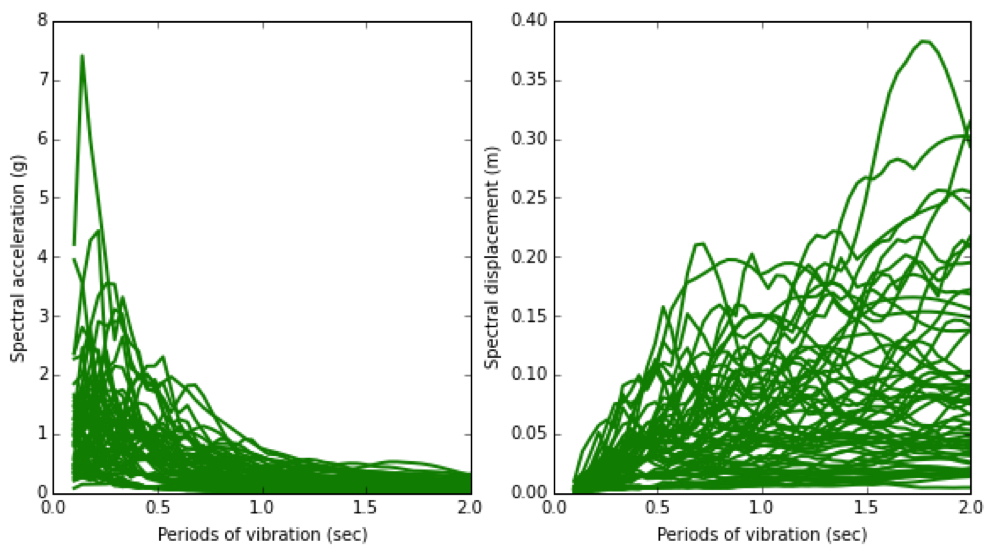
\includegraphics[width=12cm]{figures/gmrs.png}
\caption{Response spectra in terms of spectral acceleration versus period of vibration (left) and spectral displacement versus period of vibration (right).}
\label{fig:gmrs}
\end{figure}


		\subsection{Definition of damage model}
		\label{subsec:dmg_model}
		The derivation of fragility models requires the definition of a criterium to allocate one (or mutiple) structures in a set of damage states, according to their nonlinear structural response. These rules to relate structural response with physical damage can vary significantly across the literature. The displacement-based methodologies frequently adopt the strain on the concrete and steel (e.g. \cite{BorziEtAl2008b}; \cite{SilvaEtAl2013}). The vast majority of the methodologies that require equivalent linearization methods or nonlinear time history analysis adopt interstorey drifts (e.g. \cite{VamvatsikosCornell2005}; \cite{RossettoElnashai2005}), or spectral displacement calculated based on a pushover curve (e.g. \cite{Erberik2008}; \cite{SilvaEtAl2014c}). The various rules dictated by the damage model are currently being stored in a \verb=csv= file (tabular format), as described below for each type of model.

\subsubsection{Strain-based damage criterium}
\label{subsubsec:strain-dmg}
The displacement-based \citep{CrowleyEtAl2004} or mechanics-based \citep{BorziEtAl2008b} methodologies use strain levels to define a number of limit states. Thus, for each limit state, a strain for the conrete and steel should be provided. It is recognized that there is a large uncertainty in allocation of a structure into a physical damage state based on its structural response. Thus, the risk Modellers Toolkit allows the representation of the damage criterium in a probabilistic manner. This way, the parameter that establishes the damage threshold can be defined by a mean, a coefficient of variation and a probabilistic distribution (normal, lognormal or gamma) \citep{SilvaEtAl2013}. This approach is commonly used to at least assess the spectral displacement at the yieding point (\verb=Sdy=) and for the ultimate capacity (\verb=Sdu=). Other limit states can also be defined using other strain levels (e.g. \cite{CrowleyEtAl2004}), or a fraction of the yielding or ultimate displacement. For example, \cite{BorziEtAl2008b} defined light damage and collapse through the concrete and steel strains, and significant damage as $^3/_4$ of the ultimate displacement (\verb=Sdu=).\\

To use this damage criteria, it is necessary to define the parameter \verb=Type= as \verb=strain dependent= within the damage model file. Then, each limit state needs to be defined by a name (e.g. light damage), type of criterium and the adopted probabilistic model. Using the damage criteria described above (by \cite{BorziEtAl2008b}), an example of a damage model is provided in Table \ref{table:strain_dmg}. In this case, the threshold for light damage is defined at the yieding point, which in return is calculated based on the yielding strain of the steel. The limit state for collapse is computed based on the mean strain in the concrete and steel (0.0075 and 0.0225, respectively) and the a coefficient of variation (0.3 and 0.45, respectively). The remaining limit state (significant damage), is defined as fraction (0.75) of the ultimate displacement (collapse).

\begin {table}[htb]
\caption{Example of a strain dependent damage model.} 
\label{table:strain_dmg} 
\begin{center}
  \begin{tabular}{ | c | c | c | c | c |}
  \hline
Type & strain dependent &  &  &  \\ \hline
Damage States & Criteria & distribution & mean & cov  \\ \hline
light damage & Sdy & lognormal &  & 0 \\ \hline
significant damage & fraction Sdu & lognormal & 0.75 & 0 \\ \hline
collapse & strain & lognormal & 0.0075 0.0225 & 0.30 0.45 \\ \hline
  \end{tabular}
\end{center}
\end{table}

\subsubsection{Capacity curve-based damage criterium}
\label{subsubsec:strain-dmg}
Several existing studies (e.g. \cite{Erberik2008}; \cite{SilvaEtAl2014c}; \cite{CasottoEtAl2005}) have relied on capacity curves (spectral displacement versus spectral acceleration) or pushover curves (roof displacement versus base shear) to define a set of damage thresholds. In the vast majority of these studies, the various limit states are defined as a function of the displacement at the yielding point (\verb=Sdy=), the maximum spectral acceleration (or base shear), and/or of the ultimate displacement capacity (\verb=Sdu=). For this reason, the mechanism that has been implemented in the RMTK is considerably flexible, and allows users to define a set of limit states following the options below:\\

\begin{enumerate}
 \item \verb=fraction Sdy=: this limit state is defined as a fraction of the displacement at the yeilding point (\verb=Sdy=) (e.g. 0.75 of \verb=Sdy=)
 \item \verb=Sdy= this limit state is equal to the displacement at the yielding point, usually marking the initiation of structural damage.
 \item \verb=max Sa= this limit state is defined at the displcament at the maximum spectral acceleration. 
 \item \verb=mean Sdy Sdu= this limit state is equal to the mean between the displacement at the yielding point (\verb=Sdy=) and ultimate displacement capacity (\verb=Sdu=).
 \item \verb=X Sdy Y Sdu= this limit state is defined as the weigthed mean between the displacement at the yielding point (\verb=Sdy=) and ultimate displacement capacity (\verb=Sdu=). X represents the weigth associated with the former displacement, and Y corresponds to the weigth of the latter (e.g. 1 Sdy 4 sdu).
 \item \verb=fraction Sdu= this limit state is defined as a fraction of the ultimate displacement capacity (\verb=Sdu=) (e.g. 0.75 of \verb=Sdy=)
 \item \verb=Sdu= this limit state is equal to ultimate displacement capacity (\verb=Sdu=), usually marking the point beyond which structural collapse is assumed to occur.\\
\end{enumerate}

In order to create a damage model based on this criterium, it is necessary to define the parameter \verb=Type= as \verb=capacity curve dependent=. Then, each limit state needs to be defined by a name (e.g. slight damage), type of criterium (as defined in the aformentioned list) and a pottential probabilistic model (as described in the previous sub-section). An example of a damage model considering all of the possible options described in the previous list is presented in Table \ref{table:cc_dmg}, and illustrated in Figure \ref{fig:cc_damage_model}. Despite the inclusion of all of the options, a damage model using this approach may use only a few of these criteria. Moreover, some of the options (namely the first, fifth and sixth) may by used multiple times.

\begin {table}[htb]
\caption{Example of a capacity curve dependent damage model.} 
\label{table:cc_dmg} 
\begin{center}
  \begin{tabular}{ | c | c | c | c | c |}
  \hline
    Type & capacity curve dependent &  &  & \\ \hline
    Damage States & Criteria & distribution & Mean & Cov \\ \hline
    LS1 & fraction Sdy & lognormal & 0.75 & 0.0 \\ \hline
    LS2 & Sdy & normal &  & 0.0 \\ \hline
    LS3 & max Sda & normal &  & 0.0 \\ \hline
    LS4 & mean Sdy Sdu & normal &  & 0.0 \\ \hline
    LS5 & 1 Sdy 2 Sdu & normal &  & 0.0 \\ \hline
    LS6 & fraction Sdu & normal & 0.85 & 0.0 \\ \hline
    LS7 & Sdu & normal &  & 0.0 \\ \hline
  \end{tabular}
\end{center}
\end{table}

\begin{figure}[htb]
  \centering
      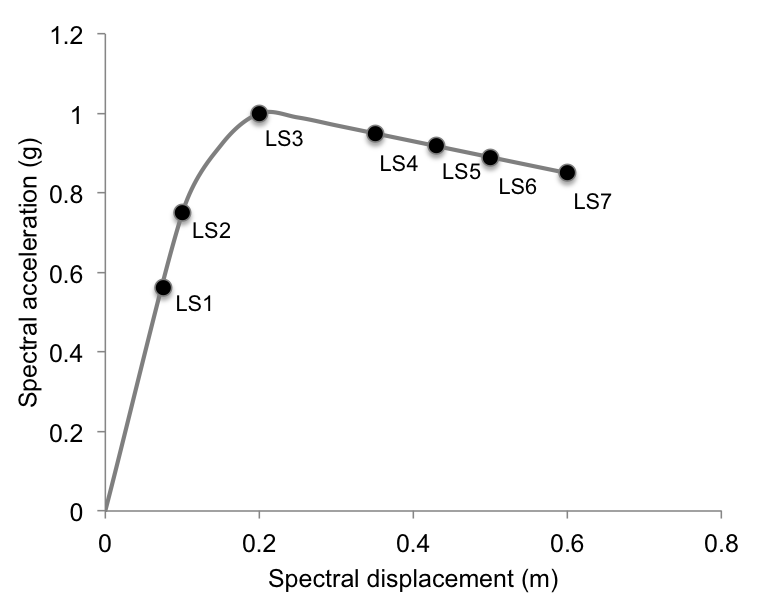
\includegraphics[width=9cm]{Figures/cc_damage_model.png}
  \caption{Representation of the possible options for the definition of the limit datates using a capacity curve.}
  \label{fig:cc_damage_model}
\end{figure}

\subsubsection{Interstorey drift-based damage criterium}
\label{subsubsec:strain-dmg}

		\subsection{Consequence model}
		\label{subsec:cons_model}
		A consequence model (also known as damage-to-loss model), establishes the relation between physical damage and a measure of fraction of loss (i.e. the ratio between repair cost and replacement cost for each damage state). These models can be used to convert a fragility model (see Section \ref{subsec:derive_fragility}) into a vulnerability function (see Section \ref{subsec:derive_fragility}). \\

Several consequence models can be found in the literature for countries such as Greece \citep{KapposEtAl2006}, Turkey \citep{BalEtAl2010}, Italy \citep{DiPasqualeandGoretti2001} or the United States \citep{FEMA2003}. The damage scales used by these models may vary considerably, and thus it is necessary to ensure compatibility with the fragility model. Consequence models are also one of the most important sources of variability, since the economical loss (or repair cost) of a group of structures within the same damage state (say moderate) can vary significantly. Thus, it is important to model this component in a probabilistic manner.\\

In the Risk Modeller's Toolkit, this model is being stored in a \verb=csv= file (tabular format), as illustrated in Table \ref{table:cons_model}. In the first column, the list of the damage states should be provided. Since the distribution of loss ratio per damage state can be modelled using a probabilistic model, the second column must be used to specify which statistical distribution should be used. Currently, \verb=normal=, \verb=lognormal= and \verb=gamma= distributions are supported. The mean and associated coefficient of variation (cov) for each damage state must be specified on the third and fourth columns, respectively. Finally, each distribution should be truncated, in order to ensure consistency during the sampling process (e.g. avoid negative loss ratios in case a \verb=normal= distribution is used, or values above 1). This variability can also be neglected, by setting the coefficient of variation (cov) to zero.

\begin {table}[htb]
\caption{Example of a consequence model.}
\label{table:cons_model}
\begin{center}
  \begin{tabular}{ | c | c | c | c | c | c |}
  \hline
Damage States & distribution & Mean & Cov & A & B\\ \hline
Slight & normal & 0.1 & 0.2 & 0 & 0.2\\ \hline
Moderate & normal & 0.3 & 0.1 & 0.2 & 0.4\\ \hline
Extensive & normal & 0.6 & 0.1 & 0.4 & 0.8\\ \hline
Collapse & normal & 1 & 0 & 0.8 & 1\\ \hline
  \end{tabular}
\end{center}
\end{table}



	\section{Model generator}
	\label{sec:model-gen}
	The methodologies currently implemented in the Risk Modeller's Toolkit require the definition of the capacity of the structure (or building class) using a capacity curve (or pushover curve). These curves can be derived using software for structural analysis (e.g. SeismoStruct, OpenSees); experimental tests in laboratories; observation of damage from previous earthquakes; and analytical methods. The Risk Modeller's Toolkit provides two simplified methodologies (DBELA - \cite{SilvaEtAl2013}; SP-BELA - \cite{BorziEtAl2008b}) to generate capacity curves, based on the geometrical and material properties of the building class (thus allowing the propagation of the building to building vartiability). Moreover, it also features a module to generate sets of capacity curves, based on the median curve (believed to be representative of the building class) and the expected variability at specific points of the reference capacity curve.

		\subsection{Generation of capacity curves using DBELA}
		\label{subsec:DBELA}
		The Displacement-based Earthquake Loss Assessment (DBELA) methodology permits the calculation of the displacement capacity of a collection of structures at a number of limit states (which could be structural or non-structural). These displacements are derived based on the capacity of an equivalent SDoF structure, following the principles of structural mechanics (\cite{CrowleyEtAl2004}; \cite{BalEtAl2010}; \cite{SilvaEtAl2013}).\\
The displacement at the height of the centre of seismic force of the original structure ($H_{CSF}$) can be estimated by multiplying the base rotation by the height of the equivalent SDoF structure ($H_{SDOF}$), which is obtained by multiplying the total height of the actual structure ($H_T$) by an effective height ratio ($ef_h$), as illustrated in Figure~\ref{fig:efh}:

\begin{figure}[htb]
  \centering
      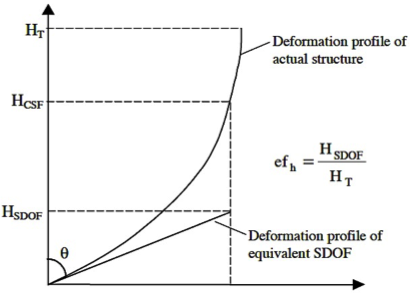
\includegraphics[width=8cm]{figures/effective_height.png}
  \caption{Definition of effective height coefficient \cite{GlaisterPinho2003}.}
  \label{fig:efh}
\end{figure}

\cite{PinhoEtAl2002} and \cite{GlaisterPinho2003} proposed formulae for estimating the effective height coefficient for different response mechanisms. For what concerns the beam sway mechanism (or distributed plasticity mechanism, as shown in Figure \ref{fig:mechanisms}), a ratio of 0.64 is proposed for structures with 4 or less storeys, and 0.44 for structures with 20 or more storeys. For any structures that might fall within these limits, linear interpolation should be employed. With regards to the column-sway mechanism (or concentrated plasticity mechanism, as shown in Figure~\ref{fig:mechanisms}), the deformed shapes vary from a linear profile (pre-yield) to a non-linear profile (post-yield). As described in \cite{GlaisterPinho2003}, a coefficient of 0.67 is assumed for the pre-yield response and the following simplified formula can be applied post-yield (to attempt to account for the ductility dependence of the effective height post-yield coefficient):

\begin{equation}
  ef_h = 0.67 - 0.17\frac{\epsilon_{s(LS_i)}-\epsilon_y}{\epsilon_{s(LS_i)}}
\end{equation}

\begin{figure}[htb]
  \centering
      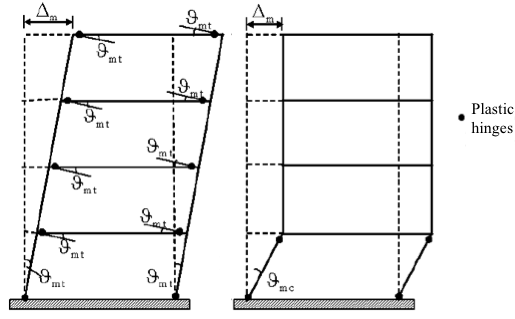
\includegraphics[width=10cm]{figures/collapse_mechanisms.png}
  \caption{Deformed profiles for beam-sway (left) and column-sway (right) mechanisms\cite{PaulayPriestley2002}.}
  \label{fig:mechanisms}
\end{figure}
The displacement capacity at different limit states (either at yield ($\delta_y$) or post-yield ($\delta_{(LSi)}$) for bare frame or infilled reinforced concrete structures can be computed using simplified formulae, which are distinct if the structure is expected to exhibit a beam- or column-sway failure mechanism. These formulae can be found in \cite{BalEtAl2010} or \cite{SilvaEtAl2013}, and their mathematical formulation is described in detail in \cite{CrowleyEtAl2004}.\\

In order to estimate whether a given frame will respond with a beam- or a column-sway mechanism it is necessary to evaluate the properties of the storey. A deformation-based index ($R$) has been proposed by \cite{AboElEzz2008} which reflects the relation between the stiffness of the beams and columns. This index can be computed using the following formula:
\begin{equation}
R = \frac{^{h_b}/_{l_b}}{^{h_c}/_{l_c}}
\end{equation}

Where $l_c$ stands for the column length. \cite{AboElEzz2008} proposed some limits for this index applicable to bare and fully infilled frame structures, as described in Table \ref{table:AboElEzz2008}.
\begin {table}[htb]
\caption{Limits for the deformation-based sway index proposed by \cite{AboElEzz2008}}
\label{table:AboElEzz2008}
\begin{center}
  \begin{tabular}{ | c | c | c |}
  \hline
    Building Typology & Beam sway & Column sway  \\ \hline
    Bare frames & R$\leq$1.0 & R>1.5 \\ \hline
    Fully infilled frames & R$\leq$1.0 & R>1.0 \\ \hline
  \end{tabular}
\end{center}
\end{table}

The calculation of the corresponding spectral acceleration is performed by assuming a perfectly elasto-plastic behaviour. Thus, the spectral displacement for the yielding point is used to derive the associated acceleration through the following formula:

\begin{equation}
Sa_i = \frac{4\pi^2Sd_i}{T_y^2}
\end{equation}

Where $T_y$ stands for the yielding period which can be calculated using simplified formulae (e.g. \cite{CrowleyPinho2004}; \cite{CrowleyPinho2006}), as further explained in Section~\ref{subsec:DBELA_Silva2013}. Due to the assumption of the elasto-plastic behaviour, the spectral acceleration for the remaining limit states (or spectral displacements) will be the same (see Figure~\ref{fig:DBELA_cc}).\\

In order to use this methodology it is necessary to define a building model, which specifies the probabilistic distribution of the geometrical and material properties. This information is currently stored in a $csv$ file (tabular format), as presented in Table~\ref{table:building_model_dbela}.

\begin {table}[htb]
\caption{Example of a building model compatible with the DBELA method.}
\label{table:building_model_dbela}
\begin{center}
  \begin{tabular}{ | l | l | l | l | l | l |}
  \hline
Structure type & bare frame &  &  &  &  \\ \hline
ductility & ductile &  &  &  &  \\ \hline
number of storeys & 3 &  &  &  &  \\ \hline
steel modulus & lognormal & 210000 & 0.01 & 0 & inf \\ \hline
steel yield strength & normal & 371.33 & 0.24 & 0 & inf \\ \hline
ground floor height & discrete & 2.8 3.1 3.2 & 0.48 0.15 0.37 & 0 & inf \\ \hline
regular floor height & lognormal & 2.84 & 0.08 & 0 & inf \\ \hline
column depth & lognormal & 0.45 & 0.12 & 0.3 & 0.6 \\ \hline
beam length & gamma & 3.37 & 0.38 & 0 & inf \\ \hline
beam depth & lognormal & 0.6 & 0.16 & 0.4 & 0.8 \\ \hline
  \end{tabular}
\end{center}
\end{table}

The \verb=structure type= can be set to \verb=bare frame= or \verb=infilled frame=, while the parameter \verb=ductility= can be equal to \verb=ductile= or \verb=non-ductile=. The variable \verb=number of storeys= must be equal to an integer defining the number of floors of the building class. The following parameters (\verb=steel modulus= , \verb=steel yield strength= , \verb=ground floor height= , \verb=regular floor height= , \verb=column depth= , \verb=beam length= , \verb=beam depth=) represent the geometrical and material properties of the building class, and can defined in a probabilistic manner. Currently, three parametric statistical models have been implemented (\verb=normal= , \verb=lognormal= and \verb=gamma=), as well as the discrete (i.e. probability mass function) model (\verb=discrete=). The model that should be used must be specified on the second column. Then, for the former type of models (parametric), the mean and coefficient of variation should be provided in the third and fourth columns, respectively. For the discrete model, the central values of the bins and corresponding probabilities of occurrence should be defined in the third and fourth columns, respectively. The last two columns can be used to truncate the probabilistic distribution between a minimum (fifth column) and maximum (sixth column) values. In order to define a parameter in a deterministic manner (i.e. no variability), the coefficient of variation for the associated attribute can be set to zero, and the same value (mean) will be used repeatedly.\\

The location of the building model and the damage model (see Section \ref{subsec:dmg_model}) should be specified in the variables \verb=building_model= and the \verb=damage_model=, respectively. The number of capacity curves that should be generated must be defined using the parameter \verb=no_assets=. Then, after importing the module \verb=DBELA=, the set of capacity curves can be generated using the following commands:

\begin{Verbatim}[frame=single, commandchars=\\\{\}, samepage=true]
building_class_model = DBELA.read_building_class_model(building_model)
assets = DBELA.generate_assets(building_class_model,no_assets)
capacity_curves = DBELA.generate_capacity_curves(assets,damage_model)
\end{Verbatim}

The first function (\verb=read_building_class_model=) processes the information about the building class; the second function (\verb=generate_assets=) uses a Monte Carlo sampling process to generate a set of synthetic structural models (each one with unique geometrical and material properties); and the final function (\verb=generate_capacity_curves=) combines the generated assets with the damage model to calculate a capacity curve per structure. Figure \ref{fig:DBELA_cc} presents a collection of capacity curves generated using this methodology.

\begin{figure}[htb]
  \centering
      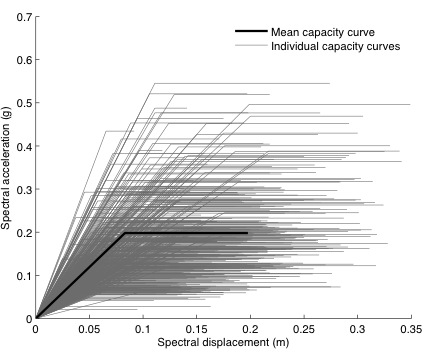
\includegraphics[width=8cm]{figures/synthethic_capacity_curves.png}
  \caption{Capacity curves for reinforced concrete bare frames generated using the DBELA methodology.}
  \label{fig:DBELA_cc}
\end{figure}

		\subsection{Generation of capacity curves using SP-BELA displacement equations}
		\label{subsec:SPBELA}
		The Simplified Pushover-based Earthquake Loss Assessment methodology \citep{BorziEtAl2008b} allows the calculation of the displacement capacity (i.e. spectral displacement) and collapse multiplier (i.e. spectral acceleration) using a mechanics-based procedure, similar to what has been proposed by \citet{CosenzaEtAl2005}. The methodology implemented in the Risk Modeller's Toolkit currently only uses the displacement capacity equations of SP-BELA for reinforced concrete frames (and does not yet estimate the collapse multiplier using the simplified pushover approach of SP-BELA). The full SP-BELA methodology will be implemented in the future, together with the similar process that has also been proposed for masonry structures \citep{BorziEtAl2008a}.\\

The original methodology as proposed by \citet{BorziEtAl2008b} considered three limit states (light damage corresponding to the yielding point, significant damage, and collapse). However, other limit states can be considered, granted that the user provides the information required to establish each limit state.\\

The spectral displacement at each limit state is calculated by firstly assessing the expected chord rotation at the associated damage threshold, and then multiplying this rotation by the height of the equivalent single degree of freedom (SDoF) system. The rotation at the yielding point ($\Theta_y$)can be calculated using the formula below, as proposed by \citet{CosenzaEtAl2005} and \citet{PanagiotakosFardis2001}:

\begin{equation}
	\Theta_y = \phi_y\frac{L_V}{3}+0.0013\left(1 + 1.5\frac{h}{L_V}\right)+0.13\phi_y\frac{d_bf_y}{\sqrt{f_c}}
\end{equation}

Where $\phi_y$ stands for the yield curvature of the section, $L_V$ represents the shear span (which for columns can be assumed as half of the inter-storey height \citep{BorziEtAl2008b}), $h$ stands for the section height, $d_b$ is the longitudinal bar diameter, and $f_y$ and $f_c$ are the strength of the steel and concrete (in MPa), respectively. The yield curvature ($\phi_y$) can be calculated using the equation proposed by \cite{PriestleyEtAl2007}:

\begin{equation}
	\phi_y = 2.14\frac{\epsilon_y}{h}
\end{equation}

Where $\epsilon_y$ represents the yield strain of the longitudinal rebars.\\

For what concerns the ultimate rotation capacity ($\Theta_u$), \cite{PanagiotakosFardis2001} proposed the following formula:

\begin{equation}
	\Theta_u = \frac{1}{\gamma_{el}}\left[\Theta_y + (\phi_u-\phi_y)L_{pl}\left(1-\frac{0.5L_pl}{L_V}\right)\right]
\end{equation}

Where $\gamma_{el}$ is 1.5 for the primary structural elements and 1 for all others \citep{BorziEtAl2008b}, $\phi_u$ stands for the ultimate curvature, and $L_pl$ is the plastic hinge length, which can be computed through the following equation:

\begin{equation}
	\phi_u = \frac{\epsilon_{cu}+\epsilon_{su}}{h}
\end{equation}

Where $\epsilon_{cu}$ and $\epsilon_{su}$ are the ultimate concrete and steel strain, respectively. These two parameters depend on the level of confinement of the reinforced concrete and expected ductility, and reasonable ranges can be found in \cite{Calvi1999}, \cite{CrowleyEtAl2004} or \cite{BalEtAl2010}.\\

Other rotation thresholds (corresponding to other limit states) can also be calculated, either through the definition of concrete and steel strains (e.g. \cite{CrowleyEtAl2004}), or as a fraction of the previously described rotations. For example, \cite{BorziEtAl2008b} defined the limit state for significant damage as $^3/_4$ of the ultimate rotation capacity ($\Theta_u$).\\

As previously mentioned, the spectral displacement at each limit state can be calculated by multiplying the respective rotation by the height of the equivalent SDoF system. This height is calculated by multiplying the total height of the structure ($H_T$) by an effective height ratio ($ef_h$). The calculation of this ratio depends on the expected failure mechanism (beam sway or column sway - see Figure~\ref{fig:mechanisms}), and its calculation has been explained in Section~\ref{subsec:DBELA}. For the yielding point, the spectral displacement can then be calculated as follows:

\begin{equation}
	\Delta_y = \Theta_yef_hH_T
\end{equation}

The displacement capacity at the remaining limit states depends on the expected failure mechanisms (as defined in Figure~\ref{fig:mechanisms}), and can be calculated using the following formulae:\\

For beam sway:

\begin{equation}
	\Delta_{LS_i} = \Delta_y + (\Theta_{LS_i} - \Theta_y)ef_hH_T
\end{equation}

for column sway:
\begin{equation}
	\Delta_{LS_i} = \Delta_y + (\Theta_{LS_i} - \Theta_y)h_p
\end{equation}

Where $h_p$ stands for the ground storey height.

The calculation of the spectral aceleration for each limit states follows the same procedure explained in the previous Section, in which an elasto-plastic behaviour is assumed, and the following formula is employed to calculate acceleration at the yielding point:

\begin{equation}
	Sa_i = \frac{4\pi^2Sd_i}{T_y^2}
\end{equation}

Where $T_y$ stands for the yielding period which is currently calculated using simplified formulae (e.g. \cite{CrowleyPinho2004}; \cite{CrowleyPinho2006}), as further explained in Section \ref{subsec:DBELA_Silva2013}, rather than based on estimating the collapse multiplier as in the original SP-BELA methodology.\\

To use this methodology it is necessary to define a building model, which specifies the probabilistic distribution of the geometrical and material properties. This information is currently stored in a $csv$ file (tabular format), as presented in Table \ref{table:building_model_spbela}.

\begin {table}[htb]
\caption{Example of a building model compatible with the SPBELA method}
\label{table:building_model_spbela}
\begin{center}
  \begin{tabular}{ | l | l | l | l | l | l |}
  \hline
Structure type & bare frame &  &  &  &  \\ \hline
ductility & ductile &  &  &  &  \\ \hline
number of storeys & 3 &  &  &  &  \\ \hline
steel modulus & lognormal & 210000 & 0.01 & 0 & $\infty$ \\ \hline
concrete strength & normal & 30 & 0.05 & 0 & $\infty$ \\ \hline
steel bar diameter & discrete & 0.01 & 1 & 0 & $\infty$ \\ \hline
steel yield strength & normal & 371.33 & 0.24 & 0 & $\infty$ \\ \hline
ground floor height & discrete & 2.8 3.1 3.2 & 0.48 0.15 0.37 & 0 & $\infty$ \\ \hline
regular floor height & lognormal & 2.84 & 0.08 & 0 & $\infty$ \\ \hline
column depth & lognormal & 0.45 & 0.12 & 0.3 & 0.6 \\ \hline
beam length & gamma & 3.37 & 0.38 & 0 & $\infty$ \\ \hline
beam depth & lognormal & 0.6 & 0.16 & 0.4 & 0.8 \\ \hline
  \end{tabular}
\end{center}
\end{table}

The definition of each parameter follows the same approach described in the previous Section for the Displacement-based Earthquake Loss Assessment (DBELA) methodology.

The location of the building model and the damage model (see Section \ref{subsec:dmg_model}) should be specified in the variables \verb=building_model= and the \verb=damage_model=, respectively. The number of capacity curves that should be generated must be defined using the parameter \verb=no_assets=. Then, after importing the module \verb=SPBELA=, the set of capacity curves can be generated using the following commands:

\begin{Verbatim}[frame=single, commandchars=\\\{\}, samepage=true]
building_class_model = SPBELA.read_building_class_model(building_model)
assets = SPBELA.generate_assets(building_class_model,no_assets)
capacity_curves = SPBELA.generate_capacity_curves(assets,damage_model)
\end{Verbatim}

The first function (\verb=read_building_class_model=) processes the information about the building class; the second function (\verb=generate_assets=) uses a Monte Carlo sampling process to generate a set of synthetic structural models (each one with unique geometrical and material properties); and the final function (\verb=generate_capacity_curves=) combines the generated assets with the damage model to calculate a capacity curve per structure. Figure \ref{fig:SPBELA_cc} presents a collection of capacity curves generated using this methodology.

\begin{figure}[htb]
  \centering
      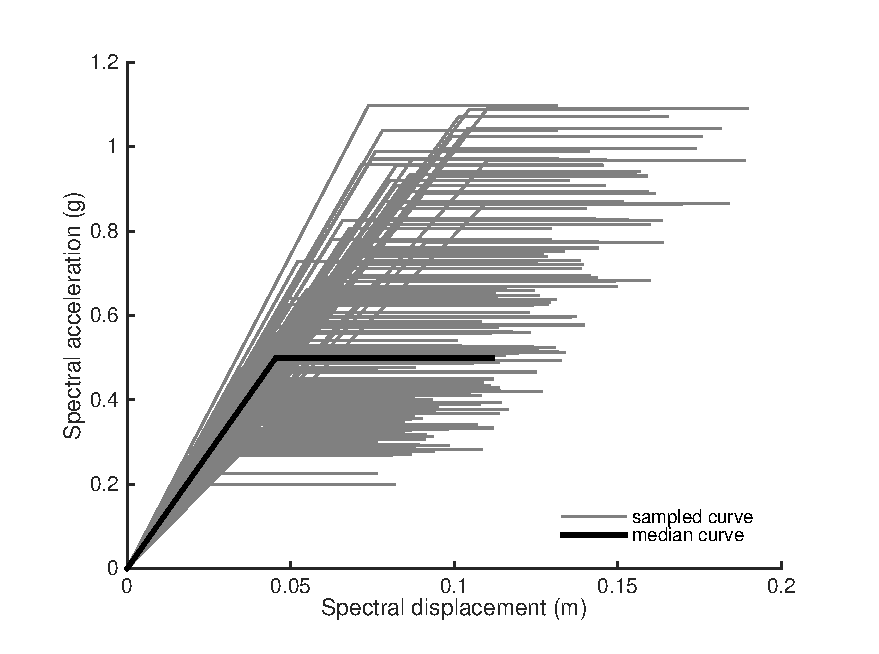
\includegraphics[width=8cm]{figures/SPBELA_cc.eps}
  \caption{Capacity curves for reinforced concrete bare frames generated using the SPBELA methodology.}
  \label{fig:SPBELA_cc}
\end{figure}

		\subsection{Generation of capacity curves using point dispersion}
		\label{subsec:dispersion}
		This module of the Risk Modeller's Toolkit allows the generation of a large number of capacity curves, based on a single median curve, and information regarding the expected dispersion at each point of the curve. \\

As an example, in a study carried out by \cite{SilvaEtAl2014b}, several capacity curves were derived for 100 reinforced concrete frames with 4 storeys without seismic provisions, as illustrated in Figure \ref{fig:set_cc}. In addition to the mean and median capacity curves, an additional capacity curve was also derived using the mean geometrical and material properties of the building class of interest. From this distribution of curves, it is possible to assess the probabilistic distribution of a number of specific points, such as the yielding or ultimate capacities. Then, once adequate statistical models have been defined for these specific points, it is possible to reproduce the the distribution of capacity curves using a Monte Carlo approach. If one assumes that such distribution could be applicable to other building classes, then it is possible to produce sets of capacity curves (as a way to propagate the building-to-building variability), based on this dispersion and a capacity curve believed to be representative of the median capacity of the building class.

\begin{figure}[htb]
  \centering
      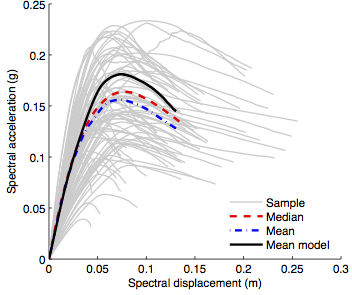
\includegraphics[width=7cm]{Figures/set_capacity_curves.png}
  \caption{Capacity curves using a displacement-based adaptive pushover approach \citep{SilvaEtAl2014b}.}
  \label{fig:set_cc}
\end{figure}

To use this methodology, it is necessary to import the module \verb=point_dispersion=. Then, the spectral acceleration and displacement of the median capacity curve should be defined in the vectors \verb=Sa= and \verb=Sd=, respectively. For each point in these vectors, it is necessary to provide the corresponding variability (as a form of a coefficient of variation), in the variables \verb=Sa_cov= and \verb=Sd_cov=. The type of probabilistic distribution that should be used must be defined using the parameter \verb=type_of_dist=. Currently this module allows \verb=normal= and \verb=lognormal=. An example of the definition of these variables is provided below. In this case, the capacity curves are being defined using three points (the yielding capacity, the point of maximum force and the ultimate displacement).

\begin{Verbatim}[frame=single, commandchars=\\\{\}, samepage=true]
Sa = [0.25, 0.45, 0.35]
Sa_cov = [0.25, 0.30, 0.30]
Sd =  [0.10, 0.20, 0.50]
Sd_cov = [0.20, 0.30, 0.45]
type_dist = 'normal'
\end{Verbatim}

Within this methodology, it is also possible to specify the correlation in the spectral acceleration (\verb=Sa_corr=) and spectral displacement (\verb=Sd_corr=). If these correlation factors are set to zero, then the sampling process is carried out independently. On the other hand, if these parameters are set to one, then a full correlation is assumed, which means, for example, if a higher displacement is sampled for the yielding point, then a large displacement will also be sampled for the remaining points. Values between zero and one will lead to intermediate situations. It is also possible to control the correlation between the spectral acceleration and displacement, using the variable \verb=SaSd_corr=.
The dispersion of the synthetic capacity curves can also be controlled through the allowed number of standard deviations above or below the median capacity curve. This aspect is controlled by the parameter \verb=truncation=, which should be equal to the maximum number of allowed standard deviations. for example, a value equal to 1 signifies that all of the generated capacity curves will be within one standard deviation of the median capacity curve. Finally, the number of capacity curves that will be generated needs to be specified using the variable \verb=no_cc=. Figure \ref{fig:dispersion_cc} illustrates 100 capacity curves generated using the data provided above.

\begin{figure}[htb]
  \centering
      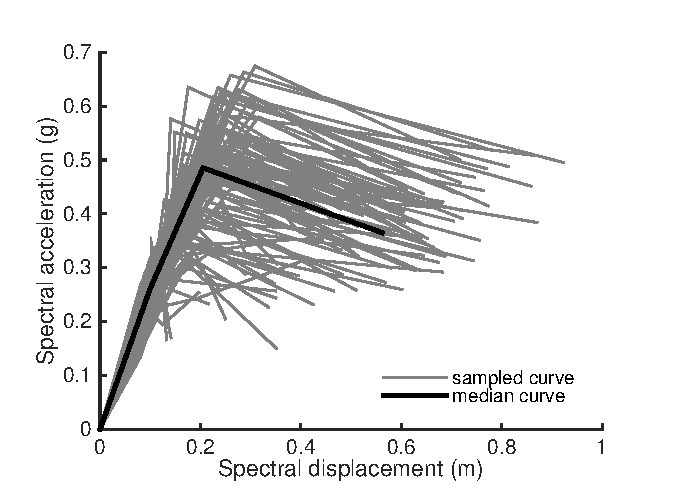
\includegraphics[width=8cm]{Figures/dispersion_cc.eps}
  \caption{Capacity curves generated using the point dispersion approach.}
  \label{fig:dispersion_cc}
\end{figure}

	\section{Conversion from MDOF to SDOF}
	\label{sec:mdof_to_sdof}
	% A conventional pushover curve describes the relation between base shear and roof displacement of a MDOF structure when an increasing lateral force is applied. The use of pushover curves in earthquake engineering somewhat originates from the pioneering work or Gulkan and Sozen [36], in which simplified SDOF models were created to represent MDOF structures and used in nonlinear static analysis. This methodology has many advantages and disadvantages that have been the focus of several studies for the past years, in particular that by Krawinkler and Seneviratna [37]. The latter stated that such approach is a valuable tool in vulnerability assessment because of its simplicity, ease of use, and reduced running time, despite its inability to reproduce certain phenomena such as viscous damping, strength deterioration or pinching effect. These authors also highlighted the constant loading pattern as one of the weakest points of this method, as it ignores some deformation modes that are propelled by dynamic response and inelastic response characteristics. This invariant loading pattern usually adopts a uniform, triangular or a first deformation mode shape. In this study, the first two patterns were considered but not the latter, because the regularity of the RC frames led to a first deformation mode approximately of a triangular shape, thus leading to the same structural behavior. Instead, a decision was taken to apply a modal loading pattern with the resulting shape from the contribution of the first three modes of vibration.
% The transformation of the pushover curve from the MDOF system to a capacity curve in terms of spectral acceleration (Sa) versus spectral displacement (Sd) for an equivalent SDOF structure can be carried out in various ways, under the condition that the deformed shape of the structure is not significantly altered during the dynamic loading. The roof displacement has been converted to Sd herein on the basis of the participation factor of the first mode of vibration, whereas the base shear has been reduced to Sa using the same factor and the first modal mass.

Several structural analysis packages allow the user to perform a reliable pushover analysis on a nonlinear model of the MDOF structure. Often, these MDOF pushover cuves need to be converted to simplified SDOF models for use in nonlinear static analysis methods. This module allows the conversion of the MDOF results into 'equivalent SDOF' results, thus making them compatible with a wide range of non-linear static procedures. At present, two methods are provided in this module for obtaining equivalent SDOF capacity curves for an MDOF system.

% A pushover curve is generated by subjecting a detailed or a carefully simplified structural model to one or more lateral load patterns and then increasing the magnitude of the total load to generate a nonlinear inelastic force-deformation relationship. The load vector is usually a representation of the load acting on the structure vibrating in its first mode .In ATC-40 Procedure A , the global parameters used are spectral acceleration and spectral displacement. Therefore a Capacity curve used in this procedure is a curve obtained by transforming the structure base shear vs. roof displacement curve into an Equivalent Single Degree of Freedom structure, acceleration vs. displacement curve .In this chapter equations needed to convert the pushover curve into a capacity curve will be developed.

		\subsection{Conversion based on one mode of vibration}
		\label{subsec:one_mode}
		This method allows the user to convert a pushover curve for an MDOF system into an equivalent SDOF capacity curve, considering the first mode of vibration only. The supplied pushover curve, which is in terms of base shear and roof displacement, is transformed into an equivalent SDOF capacity curve, which is in terms of spectral acceleration and spectral displacement. The properties of the equivalent SDOF model correspond to the properties of the first mode of vibration of the MDOF system. The roof displacement is converted to $S_d$ by normalising by the participation factor of the first mode of vibration, whereas the base shear is normalised to give $S_a$ using the the participation factor and modal mass for the first mode. Details of this conversion method can be found in \citet{ATC1996}, \citet{FEMA4402005}, and Eurocode 8 \citep{CEN2005}.

The equivalent system acceleration $S_{a-capacity}$ and displacement $S_{d-capacity}$ are calculated as:
\begin{equation}
	S_{a-capacity} = \frac{V_{b-pushover}}{M_{1}^{*} g}
\end{equation}

\begin{equation}
	S_{d-capacity} = \frac{\Delta_{roof}}{\Gamma_{1} \phi_{1, roof}}
\end{equation}

where 􏰁$\Gamma_{1}$ and $M_{1}^{*}$ are the modal participation factor and the modal mass of the first mode respectively, $\Delta_{roof}$ is the displacement of the roof, $\phi_{1, roof}$ is the roof displacement in the first mode, and $V_{b-pushover}$ is the total base shear from the pushover analysis. $\Gamma_{1}$ and $M_{1}^{*}$ are obtained using the following equations:

\begin{equation}
	\Gamma_{1} = \frac{\sideset{}{_i}\sum m_i \phi_{i,1}}{\sideset{}{_i}\sum m_i \phi_{i,1}^2}
\end{equation}

\begin{equation}
	M_{1}^{*} = \sideset{}{_i}\sum m_i \phi_{i,1}^2
\end{equation}

Now, using the first mode approximation to derive the equivalent SDOF system, it is assumed that $M_{1}^{*} \approx \frac{1}{\Gamma_{1}}$. Furthermore, we assume that the first mode shape $\phi$ has been normalised to unit amplitude at the roof, i.e., $\phi_{1, roof} = 1$. Thus, we have the following:

\begin{equation}
	S_{a-capacity} \approx \frac{V_{b-pushover}}{W} \Gamma_1
\end{equation}

\begin{equation}
	S_{d-capacity} = \frac{\Delta_{roof}}{\Gamma_1}
\end{equation}

Note that for this conversion tool, it is assumed that the base shear in the input pushover curve has already been normalised by the weight $W$ of the structure.

		\subsection{Conversion using an adaptive approach}
		\label{subsec:adaptive}
		Adaptive pushover methods have the advantage of better accounting for stiffness degradation, influence of higher mode effects, and spectral amplifications because of ground motion frequency content. In this method, instead of applying an invariant load vector, the structural properties of the model are evaluated at each step of the analysis, and the loading pattern is updated accordingly. In this way, the variation in the structural stiffness at different deformation levels, and consequently the system degradation and period elongation can be accounted for. The only apparent drawback of this methodology can be the additional computation time required to assess the structural characteristics at every step.

The equivalent system displacement $\Delta_{sys,k}$ at step $k$ is calculated as:
\begin{equation}
	\Delta_{sys,k} = \frac{\sideset{}{_i}\sum m_i \Delta_{i,k}^2}{\sideset{}{_i}\sum m_i \Delta_{i,k}}
\end{equation}
Note that $\Delta_{sys,k}$ is defined to be the inverse of the modal participation factor.

The equivalent system acceleration $\S_{a-cap,k}$ at step $k$ is calculated as:
\begin{equation}
	S_{a-cap,k} = \frac{V_{b,k}}{M_{sys,k} g}
\end{equation}

The equivalent system mass $M_{sys,k}$ is defined as:
\begin{equation}
	M_{sys,k} = \frac{\sideset{}{_i}\sum m_i \Delta_{i,k}}{M_{sys,k} g}
\end{equation}
Note that $M_{sys,k}$ is the modal mass of the system at analysis step $k$.

	\section{Direct nonlinear static procedures}
	\label{sec:direct-nsp}
	Ruiz-Garcia and Miranda (2007), Vamvatsikos and Cornell (2006) and Dolsek and Fajfar (2004) studies on the assessment of nonlinear structural response, have been integrated in three nonlinear static procedures, which are based on the use of capacity curves, resulting from nonlinear static pushover analysis, to determine directly the median seismic intensity values $\hat{S}_a$ corresponding to the attainment of a certain damage state threshold (limit state) and the corresponding dispersion $\beta_{S_a}$. These parameters are used to represent a fragility curve as the probability of the limit state capacity $C$ being exceeded by the demand $D$, both expressed in terms of intensity levels ($S_{a,ds}$ and $S_a$ respectively), as shown in the following equation:

\begin{equation}
P_{LS}(S_a) = P(C < D | S_a) = \Phi(\frac{ln S_a -ln \hat{S}_a, ds}{\beta_{S_a}})
\label{eq:fragility-definition}
\end{equation}

The methodologies implemented allow to consider different shapes of the pushover curve, multilinear and bilinear, record-to-record dispersion and dispersion in the damage state thresholds in a systematic and harmonised way.

The intensity measure to be used is $S_a$ and a mapping between any engineering demand parameter (EDP), assumed to describe the damage state thresholds, and the roof displacement should be available from the pushover analysis.

The methodologies are originally built for single building fragility curves, however the fragility curves derived for single buildings can be combined in a unique fragility curve, which considers also the inter-building uncertainty, as described in the Section~\ref{subsec:SPO2IDA}.

		\subsection{SPO2IDA (Vamvatsikos and Cornell 2006)}
		\label{subsec:SPO2IDA}
		The tool spo2ida \citep{VamvatsikosCornell2005} is capable of converting static pushover curves into 16\%, 50\% and 84\% ida curves, as shown in Figure~\ref{fig:spo2ida}, using empirical relationships from a large database of incremental dynamic analysis results.

\begin{figure}[!htbp]
\centering
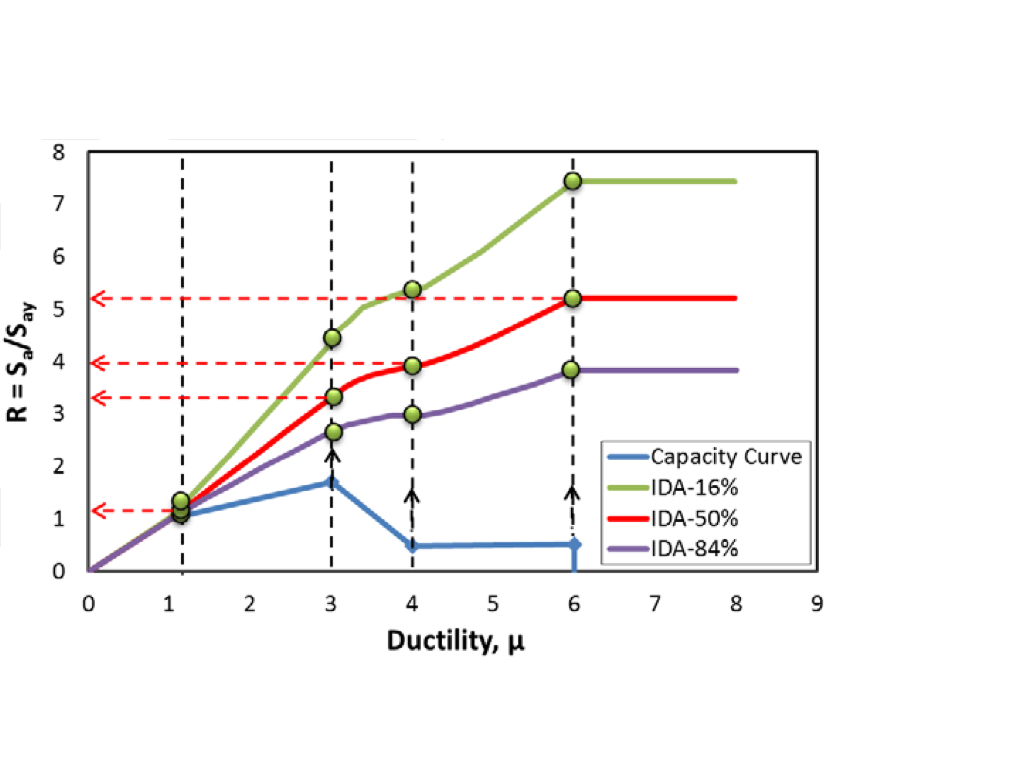
\includegraphics[width=10cm]{figures/spo2ida.jpg}
\caption{spo2ida tool: IDA curves derived from Pushover curve.}
\label{fig:spo2ida}
\end{figure}

The spo2ida tool is applicable to any kind of multi-linear capacity curve. Making use of this tool is is possible to estimate single building fragility curve and fragility curves derived for single buildings can be combined in a unique fragility curve, which considers also the inter-building uncertainty.\\

Given an idealised capacity curve the spo2ida tool uses an implicit R-$\mu$-T relation to correlate nonlinear displacement, expressed in terms of ductility $\mu$ to the corresponding median capacities in terms of the parameters R. R is the lateral strength ratio, defined as the ratio between the spectral acceleration S$_a$ and the yielding capacity of the system S$_{ay}$. Each branch of the capacity curve, hardening, softening and residual plateau, is converted to a corresponding branch of the three ida curves, using the R-$\mu$-T relation, which is a function of the hardening stiffness, the softening stiffness and the residual force. These parameters are derived from the idealised pushover capacity expressed in $\mu$-R terms, as well as the ductility levels at the onset of each branch. If some of the branches of the pushover curve are missing because of the seismic behaviour of the system, spo2ida can equally work with bilinear, trilinear and quadrilinear idealisations.\\

The result of the spo2ida routine is thus a list of ductility levels and corresponding R values at 50\%, 16\% and 84\% percentiles. For any inelastic displacement, and therefore any level of ductility $\mu$ the corresponding $R_{50\%}$, $R_{16\%}$, and $R_{84\%}$ values are found interpolating the aforementioned ida curves.
Median R and its dispersion at ductility levels corresponding to the damage thresholds ds can thus be determined, and converted into median $S_{a, ds}$ and its dispersion due to record-to-record variability $\beta_{S_{a d}}$ according to equations \ref{eq:SaR} and \ref{eq:betaR}. 

\begin{equation}
\hat{S}_{a, ds} = R_{50\%}(\mu_{ds}) S_{ay}
\label{eq:SaR}
\end{equation}
\begin{equation}
\beta_{S_{a d}} = \beta_{R(\mu_{ds})} = \frac{\ln R(\mu_{ds})_{84\%} - \ln R(\mu_{ds})_{16\%}}{2}
\label{eq:betaR}
\end{equation} 

If dispersion due to uncertainty in the limit state definition $\beta_{\theta c}$ is different from zero a Monte Carlo sampling needs to be performed to combine it with the record-to-record dispersion. Different values of ductility limit state are sampled from the  lognormal distribution with median the median value of the ductility limit state, and dispersion the input $\beta_{\theta c}$. For each of these ductilities the corresponding median $R_{50\%}$ and R$_{16\%}$, R$_{84\%}$ are found and converted into $\hat{S}_{a,ds}$ and $\beta_{S_{a d}}$ according to equation \ref{eq:SaR} and \ref{eq:betaR}. MC random S$_a$ for each MC sampled ductility limit state are computed, and their median and the dispersion are estimated. These parameters constitute the median $\hat{S}_{a,ds}$ and the total dispersion $\beta_{S_a}$ for the considered damage state. The procedure is repeated for each damage state.

\subsubsection{Multiple-Building Fragility and Vulnerability function}
\label{subsubsec:multiple-buildings}
If multiple buildings have been input to derive fragility function for a class of buildings all $\hat{S}_{a, blg}$ and $\beta_{S_a, blg}$ are combined in a single lognormal curve. A minimum of 5 buildings should be considered to obtain reliable results for the class.\\

A new issue arises when multiple buildings are considered: the S$_a$ at the fundamental period of each building should be converted to a common intensity measure, to be able to combine the different fragility functions. A common intensity measure is selected to be S$_a$ at the period T$_{av}$, which is a weighted average of the individual building fundamental periods T$_1$. Then each individual fragility needs to be expressed in terms of the common S$_a$(T$_{av}$), using a spectrum. FEMA P-695 \citep{ATC2007} far field set of 44 accelerograms (22 records for the two directions) was used to derive a mean uniform hazard spectrum, and the ratio between the S$_a$ at different periods is used to scale the fragility functions. It can be noted that the actual values of the spectrum are not important, but just the spectral shape. 
The median $\hat{S}_a$ is converted to the mean $\mu_{ln(S_a)}$ of the corresponding normal distribution ($\mu_{ln(S_a)} = ln(\hat{S}_a)$) and simply scaled to the common intensity measure as follows:

\begin{equation}
\mu_{ln(S_a), blg} = \mu_{ln(S_a), blg} S(T_{av})/ S(T_{1, blg})
\end{equation}
\begin{equation}
\beta_{S_a, blg} = \beta_{S_a, blg} S(T_{av})/ S(T_{1, blg})
\label{eq:Sa(Tav)}
\end{equation}

where $S(T_{av})/ S(T_{1, blg}$ is defined as spectral ratio. Finally the parameters of the single lognormal curve for the class of buildings, mean and dispersion, can be computed as the weighted mean of the single means and the weighted SRSS of the inter-building and intra-building standard deviation, the standard deviation of the single means and the single dispersions respectively, as shown in the following equations:

\begin{equation}
\mu_{ln(S_a), tot} = \sum_{i=0}^{n.blg} w_{blg-i} \mu_{ln(S_a), blg-i}
\label{eq:combination-lognormals-mu}
\end{equation}
\begin{equation}
\beta_{S_a, tot} = \sqrt{ \sum_{i=0}^{n.blg} w_{blg-i} ((\mu_{ln(S_a), blg-i}-\mu_{ln(S_a), tot})^2+ \beta_{S_a, blg-i}^2})
\label{eq:combination-lognormals-sigma}
\end{equation}

In order to use this methodology, it is necessary to load one or multiple capacity curves as described in Section \ref{subsec:cap_curves}.
The pushover curve input type needs to be either Base Shear vs Roof Displacement (Section \ref{subsubsec:VB-Droof}), or Base Shear vs Floor Displacements (Section \ref{subsubsec:VB-Dfloor}). It is also necessary to specify the type of shape the capacity curves want to be idealised with, using the parameter \verb=idealised_type= (either \verb=bilinear= or \verb=quadrilinear=). If the user has already at disposal an idealised multilinear pushover curve for each building, the variable \verb=Idealised= in the csv input file should be set to \verb=TRUE=, and idealised curves should be provided according to what described in section \ref{subsec:cap_curves}. Then, it is necessary to specify a damage model using the parameter \verb=damage_model= (see Section \ref{subsec:dmg_model}).\\

If dispersion due to uncertainty in the limit state definition is different from zero a Monte Carlo sampling needs to be performed to combine it with the record-to-record dispersion. The number of Monte Carlo samples should be defined in the variable \verb=montecarlo_samples=.
After importing the module \verb=SPO2IDA_procedure=, it is possible to calculate the parameter of the fragility model, median and dispersion, using the following command:

\begin{Verbatim}[frame=single, commandchars=\\\{\}, samepage=true]
fragility_model = SPO2IDA_procedure.calculate_fragility(capacity_curves,
... idealised_capacity, damage_model, montecarlo_samples, Sa_ratios,
... ida_plotflag)
\end{Verbatim}

where \verb=Sa_ratios= is the spectral ratio variable needed to combine together fragility curves for many buildings, as described in Section \ref{subsec:derive_fragility}, and \verb=ida_plotflag= indicates whether ida plots want to be displayed (\verb=ida_plotflag= = 1) or not (\verb=ida_plotflag= = 0).

		\subsection{Dolsek and Fajfar 2004}
		\label{subsec:DolsekFajfar}
		This procedure by \citep{DolsekFajfar2004} provides a simple relationship between inelastic displacement of a SDoF system and the corresponding median elastic spectral displacement value. The procedure presented herein is applicable to any kind of multi-linear capacity curve and it can be used to estimate single building fragility curve. Moreover the fragility curves derived for single buildings can be combined in a unique fragility curve, which considers also the inter-building uncertainty.\\

The relationship provided by \citep{DolsekFajfar2004} has been adapted for MDoF systems, relating the inelastic top displacement of a structure $\hat{d}_{roof}$ to the median elastic spectral acceleration value at its fundamental period of vibration $\hat{S}_{a}(T_1)$, as presented in the following equation:
 
\begin{equation}
\hat{S}_a(T_1) = \frac{4 \pi^2}{\hat{C}_R T^2 \Gamma_1 \Phi_1} \hat{d}_{roof}
\label{eq:basic_DF}
\end{equation}

where $\Gamma_1 \Phi_1$ is the first mode participation factor estimated for the first-mode shape normalised by the roof displacement. The value of C$_R$, the ratio between the inelastic and the elastic spectral displacement, is found from the following equation:

\begin{equation}
\hat{C}_{R} = \frac{\mu}{R(\mu)}
\label{eq:Cr_DF}
\end{equation}

where $\mu$ and $R$ are the median values of ductility level and the reduction factor for that level of ductility respectively. R is defined as the ratio between the spectral acceleration S$_a$ and the yielding capacity of the system S$_{ay}$.  According to the results of an extensive parametric study using three different sets of recorded and semi-artificial ground motions, \citep{DolsekFajfar2004} related the ductility demand $\mu$ and reduction factor R through the following formula:

\begin{equation}
\label{eq:mu_DF}
\mu = \frac{1}{c} (R-R_{0})+\mu_{0}
\end{equation}

In the proposed model $\mu$ is linearly dependent on R within two reduction factor intervals. The parameter c defines the slope of the R–$\mu$ relation, and it depends on the idealised pushover curve parameters (the initial period of the system T, the maximum to residual strength ratio r$_{u}$, the ductility at the onset of degradation $\mu_s$) and the corner periods T$_{c}$ and T$_{d}$. T$_{c}$ and T$_{d}$ are the corner periods between the constant acceleration and constant velocity part of the idealised elastic spectrum, and between the constant velocity and constant displacement part of the idealised elastic spectrum respectively. $R_{0}$ and $\mu_{0}$ are the values of R and $\mu$ on the capacity curve corresponding to the onset of hardening or softening behaviour, according to the following relationship:

\begin{equation}
\mu_0= 1 ... if R<=R(\mu_s); \mu_0 = \mu_s ... if R>R(\mu_s)
\end{equation}
\begin{equation}
R_0= 1 ... if R<=R(\mu_s); R_0 = R(\mu_s) ... if R>R(\mu_s)
\end{equation}

Given the parameters of the multilinear pushover curves (R$_0}$, $\mu_{0}$, r$_{u}$, $\mu_s$) and T, the median R-$\mu$ curve can be constructed using the aforementioned relationship, as presented in the following Figure.
 
\begin{figure}[!htbp]
\centering
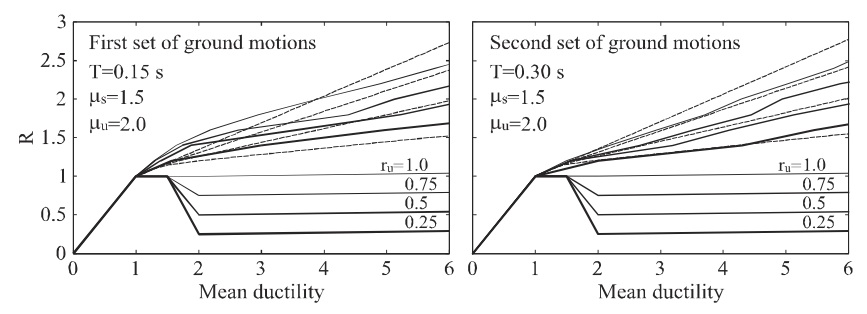
\includegraphics[width=15cm]{./figures/DF_R-mu.jpg}
\caption{R-$\mu$ curves derived from Pushover curve.}
\end{figure}

The relationship between the 16$^{th}$ and 84$^{th}$ fractiles of $\mu$ and R$_{50}$ needs to be derived using the equations from \citep{RuizGarciaMiranda2007} instead, given that \citep{DolsekFajfar2004} do not provide estimates of the dispersion of R. This is done by computing the value of record-to-record dispersion in terms of top displacement $\beta_{\theta d}$ for a number of R with eq. \ref{eq:beta_eq_RGM}, and calculating the 16$^{th}$ and 84$^{th}$ fractiles of $\mu$ ($\mu_{16\%}$ and $\mu_{84\%}$), according to the Equations \ref{eq:mu16-beta} and \ref{eq:mu84-beta}. The $\mu_{50\%}-R_{50\%}$, $\mu_{16\%}-R_{50\%}$ and $\mu_{84\%}-R_{50\%}$ curves can thus be drawn, as shown in Figure \ref{fig:R-mu}.

\begin{figure}[!htbp]
\centering
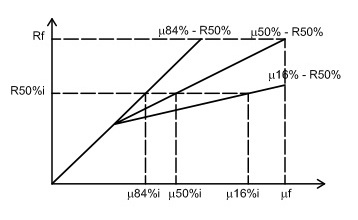
\includegraphics[width=8cm]{./figures/Rmu.jpg}
\caption{$\mu_{50\%}-R_{50\%}$, $\mu_{16\%}-R_{50\%}$ and $\mu_{84\%}-R_{50\%}$ curves}
\label{fig:R-mu}
\end{figure}

\begin{equation}
\mu_{ds,16} = \hat{\mu}_{ds} e^{-\beta_{\theta d,ds}}
\label{eq:mu16-beta}
\end{equation}
\begin{equation}
\mu_{ds,84} = \hat{\mu}_{ds} e^{\beta_{\theta d,ds}}
\label{eq:mu84-beta}
\end{equation}

For any inelastic displacement, and therefore any level of ductility $\mu$ the corresponding $R_{50\%}$, $R_{16\%}$, and $R_{84\%}$ values are found interpolating the aforementioned curves. Median R and its dispersion at ductility levels corresponding to the damage thresholds ds can thus be determined, and converted into median $S_{a, ds}$ and its dispersion due to record-to-record variability $\beta_{S_{a d}}$ according to equations \ref{eq:SaR} and \ref{eq:betaR}. \\

If dispersion in the damage state threshold is different from zero, different values of ductility limit state are sampled from the lognormal distribution with median the median value of the ductility limit state, and dispersion the input $\beta_{\theta c}$. For each of these ductilities the corresponding $R_{50\%}$, $R_{16\%}$, and $R_{84\%}$ values are found interpolating the $\mu_{50\%}-R_{50\%}$, $\mu_{16\%}-R_50\%$ and $\mu_{84\%}-R_50\%$ curves, and converted into $\hat{S}_{a,ds}$ and $\beta_{S_{a d}}$ according to Equations \ref{eq:SaR} and \ref{eq:betaR}. MC random S$_a$ for each of the MC sampled ductility limit states are computed using $\hat{S}_{a,ds}$ and $\beta_{S_{a d}}$, and their median and dispersion are estimated. These parameters constitute the median $\hat{S}_{a,ds}$ and the total dispersion $\beta_{S_a}$ for the considered damage state. The procedure is repeated for each damage state.\\

 If multiple buildings have been input to derive fragility function for a class of buildings all $\hat{S}_{a, blg}$ and $\beta_{S_a, blg}$ are combined in a single lognormal curve as described in section \ref{subsec:SPO2IDA}. \\
 
In order to use this methodology, it is necessary to load one or multiple capacity curves as described in Section \ref{subsec:cap_curves}. The capacity curves are then idealised with a bilinear elasto-plastic shape. It is also necessary to specify the type of shape the capacity curves want to be idealised with, using the parameter \verb=idealised_type= (either \verb=bilinear= or \verb=quadrilinear=). If the user has already at disposal an idealised multilinear pushover curve for each building, the variable \verb=Idealised= in the csv input file should be set to \verb=TRUE=, and idealised curves should be provided according to what described in section \ref{subsec:cap_curves}. Then, it is necessary to specify a damage model using the parameter \verb=damage_model= (see Section \ref{subsec:dmg_model}).

If dispersion due to uncertainty in the limit state definition is different from zero a Monte Carlo sampling needs to be performed to combine it with the record-to-record dispersion. The number of Monte Carlo samples should be defined in the variable \verb=montecarlo_samples=.
After importing the module DF2004, it is possible to calculate the parameter of the fragility model, median and dispersion, using the following command:

\begin{Verbatim}[frame=single, commandchars=\\\{\}, samepage=true]
fragility_model = DF2004.calculate_fragility(capacity_curves, ...
idealised_capacity, damage_model, montecarlo_samples, Sa_ratios, ...
corner_periods)
\end{Verbatim}

where \verb=Sa_ratios= is a variable needed to combine together fragility curves for many buildings, as described in Section \ref{subsec:SPO2IDA}.

		\subsection{Ruiz Garcia and Miranda 2007}
		\label{subsec:RuizGarciaMiranda}
		The research by \citep{RuizGarciaMiranda2007} provides a simple relationship for SDoF systems between inelastic displacement  and the corresponding median elastic spectral displacement value. The procedure presented herein is applicable to bilinear elasto-plastic capacity curve only and it can be used to estimate single building fragility curve. Moreover the fragility curves derived for single buildings can be combined in a unique fragility curve, which considers also the inter-building uncertainty.

The relationship provided by \citep{RuizGarciaMiranda2007} has been adapted for MDoF systems (\citep{Vamvatsikos2014}), relating the inelastic top displacement of a structure $\hat{d}_{roof}$ to the median elastic spectral displacement value at its fundamental period of vibration $\hat{S}_{d}(T)$, as presented in the following equation:

\begin{equation}
\hat{S}_d(T_1) = \frac{\hat{d}_{roof}}{\hat{C}_R \Gamma_1 \Phi_1} 
\label{eq:basic_DF}
\end{equation}

where $\Gamma_1 \Phi_1$ is the first mode participation factor estimated for the first-mode shape normalised by the roof displacement, and C$_R$ is the inelastic displacement ratio (inelastic over elastic spectral displacement), computed by \citep{RuizGarciaMiranda2007} for nonlinear SDoF systems, which is a function of the first-mode period of vibration and the relative lateral strength of the system R. Therefore the median spectral acceleration at the fundamental period of vibration $\hat{S}_{a}(T)$ turns out to be expressed as a function of top displacement according to the following equation:

\begin{equation}
\hat{S}_{a}(T) = \frac{4 \pi^2}{\hat{C}_R T^2 \Gamma_1 \Phi_1} \hat{d_{roof}}
\label{eq:Sa_RGM}
\end{equation}

Estimates of $\hat{C}_R$ parameter are provided by \citep{RuizGarciaMiranda2007}, as result of nonlinear regression analysis of three different measures of central tendency computed from 240 ground motions:

\begin{equation}
\hat{C}_R = 1 + \frac{\hat{R} - 1}{79.12 T_1 ^{1.98}}
\label{eq:Cr_RGM}
\end{equation}

where $\hat{R}$ is given by the following equation:

\begin{equation}
\hat{R} = max(0.425(1 - c + \sqrt{c^2 + 2c(2 \hat{\mu} - 1) + 1}),1)
\label{eq:R_RGM}
\end{equation}

where c = 79.12 T$^{1.98}$, and $\hat{\mu}$ is the median ductility level of interest.

Moreover \citep{RuizGarciaMiranda2007} provide an estimate of the dispersion of C$_{R}$ parameter due to record-to-record variability with Equation \ref{eq:beta_eq_RGM}, that can be assumed equal to the dispersion of $d_{roof}$, since the two quantities are proportional.

\begin{equation}
\sigma_{\ln(C_R)} = \sigma_{\ln(d_{roof})} = \beta_{\theta d} = 1.975 [\frac{1}{5.876} + \frac{1}{11.749 (T + 0.1)}] [1- \exp(-0.739 (R - 1))]
\label{eq:beta_eq_RGM}
\end{equation}

The median value of $S_a$ corresponding to any level of ductility ($d_{roof}/d_y$) can be defined combining Equation from \ref{eq:Sa_RGM} to \ref{eq:R_RGM}. The relationship between the 16$^{th}$ and 84$^{th}$ fractiles of $\mu$ and R can be drawn instead, computing $\beta_{\theta d}$ for a discretised number of R with eq. \ref{eq:beta_eq_RGM}, and calculating the 16$^{th}$ and 84$^{th}$ fractiles of $\mu$ ($\mu_{16\%}$ and $\mu_{84\%}$), according to the Equations \ref{eq:mu16-beta} and \ref{eq:mu84-beta}. $\mu_{16\%}$-$R_{50\%}$, $\mu_{50\%}$-$R_{50\%}$ obtained in such way are shown in Figure \ref{fig:Rmu}.

\begin{figure}[!htbp]
\centering
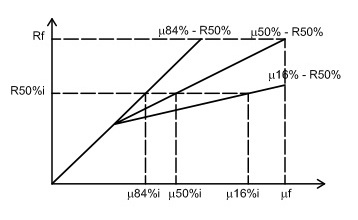
\includegraphics[width=8cm]{./figures/Rmu.jpg}
\caption{R-$\mu$ relationship.}
\label{fig:Rmu}
\end{figure}

For any inelastic displacement, and therefore any level of ductility $\mu$ the corresponding $R_{50\%}$, $R_{16\%}$, and $R_{84\%}$ values are found interpolating the aforementioned curves. Median R and its dispersion at ductility levels corresponding to the damage thresholds ds can thus be determined, and converted into median $S_{a, ds}$ and its dispersion due to record-to-record variability $\beta_{S_{a d}}$, according to equations \ref{eq:SaR} and \ref{eq:betaR}. 

If dispersion in the damage state threshold is different from zero, different values of ductility limit state are sampled from the lognormal distribution with median the median value of the ductility limit state, and dispersion the input $\beta_{\theta c}$. For each of these ductilities the corresponding $R_{50\%}$, $R_{16\%}$, and $R_{84\%}$ values are found interpolating the $\mu_{50\%}-R_{50\%}$, $\mu_{16\%}-R_50\%$ and $\mu_{84\%}-R_50\%$ curves, and converted into $\hat{S}_{a,ds}$ and $\beta_{S_{a d}}$ according to Equations \ref{eq:SaR} and \ref{eq:betaR}. MC random S$_a$ for each of the MC sampled ductility limit states are computed using $\hat{S}_{a,ds}$ and $\beta_{S_{a d}}$, and their median and dispersion are estimated. These parameters constitute the median $\hat{S}_{a,ds}$ and the total dispersion $\beta_{S_a}$ for the considered damage state. The procedure is repeated for each damage state.

If multiple buildings have been input to derive fragility function for a class of buildings all $\hat{S}_{a, blg}$ and $\beta_{S_a, blg}$ are combined in a single lognormal curve as described in section \ref{subsec:SPO2IDA}.\\

In order to use this methodology, it is necessary to load one or multiple capacity curves as described in Section \ref{subsec:cap_curves}. The pushover curve input type needs to be either Base Shear vs Roof Displacement (Section \ref{subsubsec:VB-Droof}), or Base Shear vs Floor Displacements (Section \ref{subsubsec:VB-Dfloor}). The capacity curves are then idealised with a bilinear elasto-plastic shape. If the user has already at disposal an idealised multilinear pushover curve for each building, the variable \verb=Idealised= in the csv input file should be set to \verb=TRUE=, and idealised curves should be provided according to what described in section \ref{subsec:cap_curves}. Then, it is necessary to specify a damage model using the parameter \verb=damage_model= (see Section \ref{subsec:dmg_model}).

If dispersion due to uncertainty in the limit state definition is different from zero a Monte Carlo sampling needs to be performed to combine it with the record-to-record dispersion. The number of Monte Carlo samples should be defined in the variable \verb=montecarlo_samples=.
After importing the module RGM2007, it is possible to calculate the parameter of the fragility model, median and dispersion, using the following command:

\begin{Verbatim}[frame=single, commandchars=\\\{\}, samepage=true]
fragility_model = RGM2007.calculate_fragility(capacity_curves, ...
idealised_capacity, damage_model, montecarlo_samples, Sa_ratios)
\end{Verbatim}

where \verb=Sa_ratios= is the spectral ratio variable, needed to combine together fragility curves for many buildings, as described in Section \ref{subsec:SPO2IDA}.

	\section{Record-based nonlinear static procedures}
	\label{sec:record-nsp}
	The nonlinear static procedures described in this section allow the calculation of the seismic response of a number of structures (in terms of maximum displacement of the equivalent single degree of freedom (SDoF) system), considering a set of ground motion records (see Section~\ref{subsec:gmrs}). The development of these methods involves numerical analysis of systems with particular structural and dynamic properties (e.g. periods of vibration, viscous damping, hysteretic behaviour, amongst others) and accelerograms selected for specific regions in the world (e.g. California, South Europe). For these reasons, their applicability to other types of structures and different ground motion records calls for due care. This section provides a brief description of each methodology, but users are advised to fully comprehend the chosen methodology by reading the original publications. \\

The main results of each of these methodologies is a probability damage matrix (i.e. fraction of assets per damage state for each ground motion record, represented by the variable \verb=PDM=), and the spectral displacement (i.e. expected maximum displacement of the equivalent SDoF system, represented by the variable \verb=Sds=) per ground motion record. Using the probability damage matrix (\verb=PDM=), it is possible to derive a fragility model (i.e. probability of exceedance of a number of damage states for a set of intensity measure levels - see Section~\ref{subsec:derive_fragility}), which can then be converted into a vulnerability function (i.e. distribution of loss ratio for a set of intensity measure levels - see Section \ref{subsec:derive_vulnerability}), using a consequence model (see Section \ref{subsec:cons_model}).

Table \ref{table:PDM} comprises a probability damage matrix calculated considering 100 assets and 10 ground motion records. For the purposes of this example, an extra column has been added to this table in order to display the peak ground acceleration (PGA) of each accelerogram.

\begin {table}[htb]
\caption{Example of a probability damage matrix}
\label{table:PDM}
\begin{center}
  \begin{tabular}{ | c | c | c | c | c | c |}
  \hline
    PGA & No damage & Slight damage & Moderate damage & Extensive damage & Collapse \\ \hline
    0.015 & 1.00 & 0.00 & 0.00 & 0.00 & 0.00 \\ \hline
    0.045 & 0.85 & 0.12 & 0.03 & 0.00 & 0.00 \\ \hline
    0.057 & 0.72 & 0.20 & 0.08 & 0.00 & 0.00 \\ \hline
    0.090 & 0.31 & 0.35 & 0.33 & 0.01 & 0.00 \\ \hline
    0.126 & 0.12 & 0.34 & 0.53 & 0.01 & 0.00 \\ \hline
    0.122 & 0.07 & 0.18 & 0.73 & 0.02 & 0.00 \\ \hline
    0.435 & 0.00 & 0.00 & 0.53 & 0.32 & 0.15 \\ \hline
    0.720 & 0.00 & 0.00 & 0.26 & 0.45 & 0.29 \\ \hline
    0.822 & 0.00 & 0.00 & 0.16 & 0.48 & 0.36 \\ \hline
    0.995 & 0.00 & 0.00 & 0.02 & 0.48 & 0.50 \\ \hline
  \end{tabular}
\end{center}
\end{table}


		\subsection{Vidic, Fajfar and Fischinger 1994}
		\label{subsec:VidicEtAl1994}
		This procedure aims to determine the displacements from an inelastic spectra for systems with a given ductility factor. The inelastic displacement spectra is determined by means of applying a ductility-based reduction factor (C), which depends on the natural period of the system, the given ductility factor, the hysteretic behaviour, the damping model, and the frequency content of the ground motion.\\

The procedure proposed by \citep{VidicEtAl1994} was validated by a comparison of the approximate spectra with the “exact” spectra obtained from non-linear dynamic time history analyses. Records from California and Montenegro were used as representative of “standard” ground motion, while the influence of input motion was analysed using other five groups of records (coming from different parts of the world) that represented different types of ground motions. The influence of the hysteretic models was taken into account by considering the bilinear model and the stiffness degrading Q-model. Finally, in order to analyse the effect of damping, two models were considered: “mass-proportional” damping, which assumes a time-independent damping coefficient based on elastic properties, and “instantaneous stiffness-proportional” damping, which assumes a time-dependent damping coefficient based on tangent stiffness. For most cases, a damping ratio of 5\% was assumed, although for some systems a value of 2\% was adopted.\\

It is possible to derive approximate strength and displacement inelastic spectra from an elastic pseudo-acceleration spectrum using the proposed modified spectra. In the medium and long-period region, it was observed that the reduction factor is slightly dependant on the period T and is roughly equal to the prescribed ductility ($\mu$). However, in the short-period region, the factor C strongly depends on both T and $\mu$. The influence of hysteretic behaviour and damping can be observed for the whole range of periods. Based on this, a bilinear curve was proposed. Starting in C = 1, the value of C increases linearly along the short-period region up to a value approximately equal to the ductility factor. In the medium- and long-period range, the C-factor remains constant. This is mathematically expressed by the following relationships:


\begin{equation}
C_\mu = \left\{
\begin{matrix}
  c_{1}\left(\mu-1\right)^{c_{R}}\frac{T}{T_{0}} + 1, & T\leq T_{0}  \\
  c_{1}\left(\mu-1\right)^{c_{R}} + 1 & T>T_{0}
 \end{matrix}
 \right.
\end{equation} 

where: 
\begin{equation}
T_0 = c_2\mu^{c_T}T_c
\end{equation} 

And $T_c$ stands for the characteristic spectral period and $c_1$, $c_2$, $c_R$, $c_T$ are constants dependant on the hysteretic behaviour and damping model, as defined in Table \ref{table:VidicEtAl}.

\begin {table}[htb]
\caption{Paramereters for the estimation of the reduction factor C proposed by \citep{VidicEtAl1994}} 
\label{table:VidicEtAl} 
\begin{center}
  \begin{tabular}{ | c | c | c | c | c | c |}
    \hline
    Hysteresis model & Damping model & $c_1$ & $c_2$ & $c_R$ & $c_T$ \\ \hline
    Q & Mass & 1.00 & 0.65 & 1.00 & 0.30 \\ \hline
    Q & Stiffness & 0.75 & 0.65 & 1.00 & 0.30 \\ \hline
    Bilinear & Mass & 1.35 & 0.75 & 0.95 & 0.20 \\ \hline
    Bilinear & Stiffness & 1.10 & 0.75 & 0.95 & 0.20 \\ \hline
  \end{tabular}
\end{center}
\end{table}

In order to use this methodology, it is necessary to load one or multiple capacity curves as described in Section \ref{subsec:cap_curves}, as well as a set of ground motion records as explained in Section \ref{subsec:gmrs}. Then, it is necessary to specify a damage model using the parameter \verb=damage_model= (see Section \ref{subsec:dmg_model}), and a damping ratio using the parameter \verb=damping=. It is also necessary to specify the type of hysteresis (\verb=Q= or \verb=bilinear=) and damping (\verb=mass= or \verb=stiffness=) models as defined in Table \ref{table:VidicEtAl}, using the parameters \verb=hysteresis_model= and \verb=damping_model=, respectively. After importing the module \verb=vidic_etal_1994=, it is possible to calculate the distribution of structures across the set of damage state for each ground motion record using the following command:

\begin{Verbatim}[frame=single, commandchars=\\\{\}, samepage=true]
PDM, Sds = vidic_etal_1994.calculate_fragility(capacity_curves,gmrs,...
damage_model,damping)
\end{Verbatim}

Where \verb=PDM= (i.e. probability damage matrix) represents a matrix with the number of structures in each damage state per ground motion record, and \verb=Sds= (i.e. spectral displacements) represents a matrix with the maximum displacement (of the equivalent SDOF) of each structure per ground motion record. the variable PDM can then be used to calculate the mean fragility model as described in Section \ref{subsec:derive_fragility}.





		\subsection{Lin and Miranda 2008}
		\label{subsec:LinMiranda2008}
		This methodology estimates the maximum inelastic displacement of an existing structure based on the maximum elastic displacement response of its equivalent linear system without the need for iterations, based on the strength ratio R (instead of the most commonly used ductility ratio).\\

In order to evaluate an existing structure, a pushover analysis should be conducted in order to obtain the capacity curve. This curve should be bilinearised in order to obtain the yield strength, fy, the postyield stiffness ratio, $\alpha$, and the strength ratio, R. With these parameters, along with the initial period of the system, it is possible to estimate the optimal period shift (i.e. the ratio between the period of the equivalent linear system and the initial period) and the equivalent viscous damping, $\xi$eq, of the equivalent linear system, using the following relationships derived by \citep{LinMiranda2008}.
	 
\begin{equation}
\frac{T_{eq}}{T_{0}} = 1 + \frac{m_1}{T_0^{m_2}}\left(R^{1.8}-1\right)
\end{equation} 

\begin{equation}
\xi_{eq} = \xi_{0} + \frac{n_1}{T_0^{n_2}}\left(R-1\right)
\end{equation}   

Where the coefficients m1, m2, n1, and n2 depend on the postyield stiffness ratio, as shown in the following Table \ref{table:LinMiranda2008}.

\begin {table}
\caption{Paramereters for the estimation of the reduction factor C proposed by \citep{LinMiranda2008}} 
\label{table:LinMiranda2008} 
\begin{center}
  \begin{tabular}{ | c | c | c | c | c |}
    \hline
    $\alpha$ & $m_1$ & $m_2$ & $n_1$ & $n_2$ \\ \hline
    0\% & 0.026 & 0.87 & 0.016 & 0.84 \\ \hline
    5\% & 0.026 & 0.65 & 0.027 & 0.55 \\ \hline
    10\% & 0.027 & 0.51 & 0.031 & 0.39 \\ \hline
    20\% & 0.027 & 0.36 & 0.030 & 0.24 \\ \hline
  \end{tabular}
\end{center}
\end{table}

Using $\xi$eq and the damping modification factor, B (as defined in Table 15.6-1 of NEHRP-2003), it is possible to construct the reduced displacement spectrum, Sd(T, $\xi$eq) from which the maximum displacement demand (i.e. the displacement corresponding to the equivalent system period) can be obtained, using the following equation:
	  
In order to use this methodology, it is necessary to load one or multiple capacity curves as described in Section \ref{subsec:cap_curves}, as well as a set of ground motion records as explained in Section \ref{subsec:gmrs}. Then, it is necessary to specify a damage model using the parameter \verb=damage_model= (see Section \ref{subsec:dmg_model}). After importing the module \verb=lin_miranda_2008=, it is possible to calculate the distribution of structures across the set of damage state for each ground motion record using the following command:

\begin{Verbatim}[frame=single, commandchars=\\\{\}, samepage=true]
PDM, Sds = lin_miranda_2008.calculate_fragility(capacity_curves,gmrs,...
damage_model,damping)
\end{Verbatim}

Where \verb=PDM= (i.e. probability damage matrix) represents a matrix with the number of structures in each damage state per ground motion record, and \verb=Sds= (i.e. spectral displacements) represents a matrix with the maximum displacement (of the equivalent SDOF) of each structure per ground motion record. the variable PDM can then be used to calculate the mean fragility model as described in Section \ref{subsec:derive_fragility}.






		\subsection{Miranda (2000) for firm soils}
		\label{subsec:Miranda}
		This study by \cite{Miranda2000} aims to quantify the influence of soil conditions, earthquake magnitude, and epicentral distance on the inelastic displacement ratios, $C_\mu$. For two systems with the same mass and period of vibration that have been subjected to the same earthquake ground motion. $C_\mu$ can be defined as the ratio of the maximum lateral inelastic displacement demand of one to the maximum lateral elastic displacement demand on the other, as shown in the following equation:

\begin{equation}
C_\mu = \frac{\Delta_{inelastic}}{\Delta_{elastic}}
\end{equation}

In this study, 264 earthquake acceleration time histories recorded in California (USA) for 12 different events were used. In order to investigate the effect of the soil conditions, the records were classified into three groups: the first one consisted of ground motions recorded on stations located on rock (i.e. average shear-wave velocities >760 m/s). The second group included the records registered on stations on very dense soil or soft rock (i.e. average shear-wave velocities between 360 m/s and 760 m/s). Finally, the third group consisted of ground motion records from stations located on stiff soil (i.e. average shear-wave velocities between 180 m/s and 360 m/s).\\
It was observed that for periods longer than about 1.0 s, the mean inelastic displacement ratios are approximately equal to 1, meaning that, on average, the maximum inelastic displacements are equal to the maximum inelastic displacements. On the other hand, for periods smaller than 1.0 s, the mean inelastic displacement ratios are larger than 1 and strongly depend on the period of vibration and on the level of inelastic deformation.
The results of the investigation yielded that for the sites under consideration (i.e. average shear-wave velocities higher than 180 m/s) neither the soil conditions, nor the earthquake magnitude, nor the distance to rupture cause significant differences on the value of $C_\mu$. However, if directivity effects are taken into consideration, the inelastic displacement ratios for periods between 0.1 s and 1.3 s can be larger than those estimated for systems not affected by directivity.\\

Based on the results of the mean inelastic displacement ratios, nonlinear regression analyses were conducted to estimate the following simplified expression for the inelastic displacement ratio of a system:

\begin{equation}
C_\mu = \left[1+\left(\frac{1}{\mu}-1\right)exp\left(-12T\mu^{-0.8}\right)\right]^{-1}
\end{equation}

Where $\mu$ = displacement ductility ratio and T = period of vibration.\\
In order to use this methodology, it is necessary to load one or multiple capacity curves and a set of ground motion records, as explained in Section \ref{subsec:cap_curves} and \ref{subsec:gmrs}, respectively. Then, it is necessary to specify a damage model using the parameter \verb=damage_model= (see Section \ref{subsec:dmg_model}), and a damping ratio using the parameter \verb=damping=. After importing the module \verb=miranda_2000_firm_soils=, it is possible to calculate the distribution of structures across the set of damage states for each ground motion record using the following command:

\begin{Verbatim}[frame=single, commandchars=\\\{\}, samepage=true]
PDM, Sds = miranda_2000_firm_soils.calculate_fragility(capacity_curves,...
gmrs,damage_model,damping)
\end{Verbatim}

Where \verb=PDM= (i.e. probability damage matrix) represents a matrix with the number of structures in each damage state per ground motion record, and \verb=Sds= (i.e. spectral displacements) represents a matrix with the maximum displacement (of the equivalent SDoF) of each structure per ground motion record. The variable PDM can then be used to calculate the mean fragility model as described in Section \ref{subsec:derive_fragility}.

		\subsection{N2 (EC8, CEN 2005)}
		\label{subsec:N2}
		This simplified nonlinear procedure has been firstly proposed by Fajfar, and it is capable of estimating the seismic response of structures using capacity curves (for the equivalent SDOF) and response spectra. It is somehow similar to the well-known Capacity Spectrum Method (see Section ), but it does not require an iterative process and instead of elastic overdamped spectra, it uses inelastic response spectra. This method is part of recommendations of the Eurocode 8 \citep{CEN2005} for the seismic design of new structues, and the capacity curves are usually simplified by a elasto-perfectly plastic relationship.\\
To estimate the target displacement ($\delta_t$) within this methodology, it is necessary to assess whether the SDOF structure is in the short-period or medium/long-period ranges. To do so, it is necessary to compare the fundamental period of vibration of the structure with the corner period of the ground motion record. If the structure is in the latter category, it is assumed that the target displacement is equal to the elastic spectral displacement for the fundamental period of the idealized SDOF. If on the other hand it is located in the short-period range, a procedure is carried out to evaluate whether the capacity of the SDOF at the yielding point (taken from the bilinear curve) is lower than the spectral acceleration response for the same period. If this is verified, then the structure is assumed to have an elastic response and once again, the target displacement will be equal to the elastic spectral displacement for the fundamental period. In case the capacity is lower than the response for the yielding point, the structure is assumed to have an inelastic response and the following formula is employed to determine the target displacement:
\begin{equation}
\delta_t = \frac{Sd(T_{el})}{q_u}\left(1+(q_u-1)\frac{T_c}{T_{el}}\right)Sd(T_{el})
\end{equation}
Where $Sd(T_{el})$ stands for the spectral displacement for the fundamental period of the idealized SDOF ($T_{el}$), $T_c$ stands for the corner period and $q_u$ represents the ratio between the spectral acceleration for $T_{el}$ and the acceleration at the yielding point.\\

It is important to understand that this methodology has been developed originally to be combined with a design or code-based response spectrum, and not with a spectrum derived from real ground motion records. For this reason, its employment in the derivation of fragility functions calls for due care. For instance, the estimation of $T_c$ (which is a fundamental parameter within this methodology) when considering accelerograms is not a trivial task, and various proposals can be found in the literature. For the sake of simplicity, a decision was made to adopt the formula recommended by the \cite{ASCE2010} which defines:

\begin{equation}
T_c = \frac{Sa(T=1.0s)}{Sa(T=0.2s)}
\end{equation}

Despite these caveats, it is worth mentioning that a recent study \citep{SilvaEtAl2014b} compared its performance in the derivation of vulnerability functions against nonlinear time history analyses, and concluded that reasonable results can still be obtained.\\

In order to use this methodology, it is necessary to load one or multiple capacity curves and a set of ground motio nrecords, as explained in Section \ref{subsec:cap_curves} and \ref{subsec:gmrs}, respectively. Then, it is necessary to specify a damage model using the parameter \verb=damage_model= (see Section \ref{subsec:dmg_model}), and a damping ratio using the parameter \verb=damping=. After importing the module \verb=N2Method=, it is possible to calculate the distribution of structures across the set of damage states for each ground motion record using the following command:

\begin{Verbatim}[frame=single, commandchars=\\\{\}, samepage=true]
PDM, Sds = N2Method.calculate_fragility(capacity_curves,gmrs,...
damage_model,damping)
\end{Verbatim}

Where \verb=PDM= (i.e. probability damage matrix) represents a matrix with the number of structures in each damage state per ground motion record, and \verb=Sds= (i.e. spectral displacements) represents a matrix with the maximum displacement (of the equivalent SDOF) of each structure per ground motion record. the variable PDM can then be used to calculate the mean fragility model as described in Section \ref{subsec:derive_fragility}.


		\subsection{Capacity Spectrum Method (FEMA, 2005)}
		\label{subsec:CSM}
		The capacity spectrum method (CSM) was initially proposed by \citep{FreemanEtAl1975}, and it represents a simplified methodology for many purposes such as the evaluation of a large inventory of buildings, structural assessment of new or existing buildings or to identify the correlation between damage states and levels of ground motion. \citet{ATC1996} proposes three different procedures (A, B and C) for the application of the Capacity Spectrum Method. However, procedure B adopts some simplifications that might not always be valid and procedure C has a very strong graphical component, making it difficult for systematic applications. Hence, procedure A, which is characterized by its intuitiveness and simplicity, has been implemented in the RMTK.\\

This procedure iteratively compares the capacity and the demand of a structure, using a capacity curve (for the equivalent SDoF) and a damped response spectrum, respectively. The ground motion spectrum is computed for a level of equivalent viscous damping that is estimated as a function of the displacement at which the response spectrum crosses the capacity curve, in order to take into account the inelastic behaviour of the structure. Iterations are needed until there is a match between the equivalent viscous damping of the structure and the damping applied to the spectrum. The final intersection of these two curves approximates the target displacement response of the structure. This result is presented in Figure~\ref{fig:per_point} for a "weak" and a "strong" ground motion record. \\

\begin{figure}[htb]
  \centering
      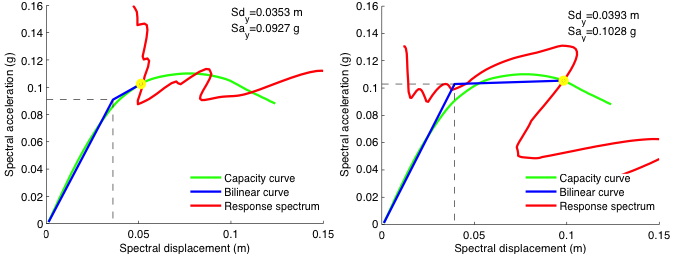
\includegraphics[width=12cm]{figures/performance_points.png}
  \caption{Assessment of the target displacement for "weak" (left) and "strong" (strong) ground motion record.}
  \label{fig:per_point}
\end{figure}

The initial proposal of this method was heavily criticized due to its tendency to underestimate the deformation of the structures, which was mostly related with the model employed to calculate the equivalent viscous damping (e.g. \cite{Fajfar1999}; \cite{ChopraGoel2010}). Thus, in \cite{FEMA4402005}, some modifications were proposed regarding the calculation of this component. Furthermore, several other models relating an equivalent viscous damping ratio ($\xi_{eq}$) with a ductility level ($\mu$) have been proposed in the last decades, and implemented in the RMTK. The following list describes these models, and specifies the code that must be defined in the variable \verb=damping_model= in order to follow the associated model in the vulnerability calculations.\\

\begin{itemize}
\item \cite{FEMA4402005}: This model assumes different expressions to calculate the equivalent viscous damping ratio depending on the ductility level, hysteretic model and post-elastic stiffness. However, for the sake of simplicity, approximate equations have been proposed to calculate $\xi_{eq}$ with any capacity curve, that only depends on the level of ductility, as described below:\\

For $1.0 < \mu < 4.0$:
\begin{equation}
	\xi_{eq} = \xi_0 + 0.049\left(\mu-1\right)^2-0.01\left(\mu-1\right)^3
\end{equation}

For $4.0 \le \mu \le 6.5$:
\begin{equation}
	\xi_{eq} = \xi_0 + 0.14 + 0.0032 \left(\mu-1\right)
\end{equation}

For $ \mu > 6.5$:
\begin{equation}
	\xi_{eq} = \xi_0 + 0.19\left[\frac{0.64\left(\mu-1\right)-1}{\left[0.64\left(\mu-1\right)\right]^2}\right]\left(\frac{T_{eff}}{T_0}\right)^2
\end{equation}

Where $\xi_0$ stands the initial elastic viscous damping ratio, and $T_{eff}$ represents the effective period, which for ductility above 6.5 can be calculated using the following expression:

\begin{equation}
	T_{eff} = \left\{0.89\left[\sqrt{\frac{(\mu-1)}{1+0.05(\mu-2)}}\right]+1\right\}T_0
\end{equation}

In order to use this model, the variable \verb=damping_model= must be set to \verb=FEMA_2005=.\\

\item \cite{Kowalsky1994}: This model establishes a relationship between the equivalent viscous damping ratio and a ductility level and a post-yield stiffness ratio $\alpha$, as defined by the following equation:

\begin{equation}
\xi_{eq} = \xi_0 + \frac{1}{\pi}\left[1-\frac{(1-\alpha)}{\sqrt{\mu}} - \alpha\sqrt{\mu} \right]
\end{equation}

In order to use this model, the variable \verb=damping_model= must be set to \verb=Kowalsky_1994=.\\

\item \citep{Iwan1980}: This model was developed using a limited number of ground motion records and a single hysteretic model, leading to the following equation:

\begin{equation}
	\xi_{eq} = \xi_0 + 0.0587\left(\mu-1\right)^0.371
\end{equation}

In order to use this model, the variable \verb=damping_model= must be set to \verb=Iwan_1980=.\\

\item \cite{GulkanSozen1974}:This model was derived considering the Takeda hysteretic for elasto-plastic systems calibrated with experimental shaking-table results of a number of reinforced concrete frames. The equivalent viscous damping ratio is calculated using the following ductility-dependent formula:

\begin{equation}
	\xi_{eq} = \xi_0 + 0.2\left(1- \frac{1}{\sqrt{\mu}}\right)
\end{equation}

In order to use this model, the variable \verb=damping_model= must be set to \verb=Gulkan_Sozen_1974=.\\

\item \cite{PriestleyEtAl2007}: These Authors proposed different models depending on the structure type. Currently, three models proposed by this study have been implemented, as described below: \\

For reinforced concrete frame structures:

\begin{equation}
	\xi_{eq} = 0.05 + 0.565\left(\frac{\mu-1}{\pi\mu}\right)
\end{equation}

To use this model set the variable \verb=damping_model= to \verb=Priesley_et_al2007_frames=.\\

For reinforced concrete walls structures:

\begin{equation}
\xi_{eq} = 0.05 + 0.444\left(\frac{\mu-1}{\pi\mu}\right)
\end{equation}

To use this model set the variable \verb=damping_model= to \verb=Priesley_et_al2007_walls=.\\

For steel structures:

\begin{equation}
	\xi_{eq} = 0.05 + 0.577\left(\frac{\mu-1}{\pi\mu}\right)
\end{equation}

To use this model set the variable \verb=damping_model= to \verb=Priesley_et_al2007_steel=.\\

\item \cite{Calvi1999}: This Author proposed a relationship between the equivalent viscous damping ratio and ductility following the expression below:

\begin{equation}
	\xi_{eq} = \xi_0 + a\left(1-\frac{1}{\mu^b}\right)
\end{equation}

Where \verb=a= and \verb=b= are constants that vary between 20 and 30, and 0.5 and 1, respectively, depending on the hysteretic properties of the structure. Thus, this model can be employed for various structure types, by adjusting these two constants. Given the fact that most of the current damping models have been derived or calibrated for reinforced concrete structures, a decision was made to adjust these parameters for the assessment of masonry structures. The \verb=a= and \verb=b= constants have been set to 25 and 0.5, respectively, as proposed by \cite{BorziEtAl2008a}. Nonetheless, due to the open and transparent architecture of the RMTK, any user can modify these parameters.\\

In order to use this model, the variable \verb=damping_model= must be set to \verb=Calvi_1999=.\\

\end{itemize}
The performance point (or target displacement) calculated within this methodology is equivalent to what would be obtained by subjecting the equivalent single degree of freedom oscilator to a nonlinear time history analysis. Then, estimated target displacement can be used to allocate the structure in a damage state, based on a pre-established set of displacement thresholds. This process can be repeated several times considering other ground motion records, as well as structures (i.e. building class).\\

In order to use this methodology, it is necessary to load one or multiple capacity curves and a set of ground motion records, as explained in Section~\ref{subsec:cap_curves} and \ref{subsec:gmrs}, respectively. Then, it is necessary to specify a damage model using the parameter \verb=damage_model= (see Section~\ref{subsec:dmg_model}), and a damping ratio using the parameter \verb=damping=. After importing the module \verb=capacitySpectrumMethod=, it is possible to calculate the distribution of structures across the set of damage states for each ground motion record using the following command:

\begin{Verbatim}[frame=single, commandchars=\\\{\}, samepage=true]
PDM, Sds = capacitySpectrumMethod.calculate_fragility(capacity_curves,...
gmrs,damage_model,damping)
\end{Verbatim}

Where \verb=PDM= (i.e. probability damage matrix) represents a matrix with the number of structures in each damage state per ground motion record, and \verb=Sds= (i.e. spectral displacements) represents a matrix with the maximum displacement (of the equivalent SDoF) of each structure per ground motion record. The variable PDM can then be used to calculate the mean fragility model as described in Section~\ref{subsec:derive_fragility}.





		\subsection{DBELA (Silva et al. 2013)}
		\label{subsec:DBELA_Silva2013}
		The Displacement-based Earthquake Loss Assessment (DBELA) methodology builds upon the urban assessment methodology proposed by \cite{Calvi1999}, in which the principles of structural mechanics and seismic response of buildings are used to estimate the seismic vulnerability of classes of buildings. The current implementation of the RMTK is only compatible with bare or infilled frame reinforced concrete structures.\\

In this method, the displacement capacity and demand for a number of limit states needs to be calculated. Each limit state marks the threshold between the levels of damage that a building might withstand, usually described by a reduction in strength or by exceedance of certain displacement/drift levels. Once these parameters are obtained, the displacement capacity of the first limit state is compared with the respective demand. If the demand exceeds the capacity, the next limit states need to be checked successively, until the demand no longer exceeds the capacity and the building damage state can be defined. If the demand also exceeds the capacity of the last limit state, the building is assumed to have collapsed. This procedure is schematically depicted in Figure \ref{fig:DBELA_scheme}, in which the capacities for three limit states are represented by $\Delta_i$ and the associated demand by $Sd_i$. In this example, the demand exceeds the capacity in the first and second limit state but not in the third limit state, thus allocating the building to the third damage state.

\begin{figure}[htb]
  \centering
      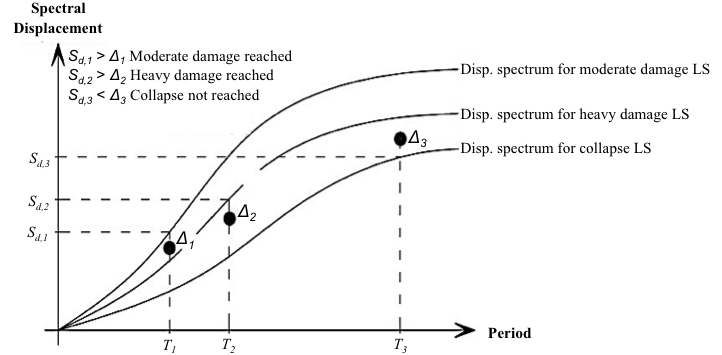
\includegraphics[width=12cm]{Figures/DBELA_scheme.png}
  \caption{Comparison between limit state capacity and the associated demand (adapted from \cite{BalEtAl2010}).}
  \label{fig:DBELA_scheme}
\end{figure}

The calculation of the displacement capacity at each limit state is explained in the Model Generation Section (\ref{sec:model-gen}), as this methodology can be employed to generate large sets of capacity curves (Sa versus Sd), which can be combined with other methodologies besides DBELA to derive fragility functions. Instead, this section is focused on describing how the seismic demand is handled in this methodology.\\ 

The demand is represented by a displacement spectrum which can be described as the expected displacement induced by an earthquake on a single-degree-of-freedom (SDOF) oscillator with a given period of vibration and viscous damping. This demand is initially calculated for a 5\% viscous damping, and later modified for each limit state using a correction factor ($\eta$), representative of the equivalent viscous damping and ductility at the associated damage state. In the Eurocode 8 \citep{CEN2005}, the following equation is proposed for the calculation of the correction factor:

\begin{equation}
\eta_{LS_i} = \sqrt{\frac{10}{5+\xi_{eq_i}}}
\end{equation}

Where $\xi_{eq_i}$ stands for the equivalent viscous damping at the limit state $i$. Although in theory there is a multitude of damping models in the literature that could be used to calculate this equivalent viscous damping (see Section \ref{subsec:CSM} for a description of the damping models implemented within the Capacity Spectrum Method), this method has been tested following the proposals by \cite{PriestleyEtAl2007} for reinforced concrete frames (e.g. \cite{BalEtAl2010} \cite{SilvaEtAl2013}). This model uses the following equation: 

\begin{equation}
\xi_{eq} = 0.05 + 0.565\left(\frac{\mu-1}{\pi\mu}\right)
\end{equation}

Where $\mu_i$ stands for the ductility at the limit state $i$ (assumed as the ratio between $\Delta_i$ and $\Delta_y$). More accurate approaches have recently been proposed to estimate the correction factors ($\eta$), considering additional parameters, such as the magnitude or source-to-site distance \citep{RezaeianEtAl2012}.\\

With regards to the calculation of the yielding period ($T_y$) for bare frame structures, \cite{CrowleyPinho2004} and \cite{CrowleyEtAl2008} proposed a relationship between the period and the total height ($H_T$) of $0.10H_T$ and $0.07H_T$ for structures without and with lateral load design, respectively. For infilled frames, a relation equal to $0.06H_T$ has been recommended by \cite{CrowleyPinho2006} for structures without lateral load design. The elongated period of vibration for any of the limit states ($T_{LS_i}$) can be computed using the following formula:

\begin{equation}
T_{LS_i} = T_y\sqrt{\frac{\mu_{i}}{1+\alpha\mu_{i}-\alpha}}
\end{equation}

where $\alpha$ stands for the post-yield stiffness ratio. In cases where this ratio can be assumed as zero, the relation between $T_{LS_i}$ and $T_y$ will depend purely on the limit state ductility as follows:

\begin{equation}
T_{LS_i} = T_y\sqrt{\mu_{i}}
\end{equation}

In order to use this methodology, it is necessary to first assess the capacity displacement of one or multiple assets, following the DBELA approch explained in Section \ref{subsec:DBELA} (Model Generator). Moreover, a set of ground motion records and a damage model should be provided, as explained in Section \ref{subsec:gmrs} and \ref{subsec:dmg_model}), respectively. The type of structures that are being evaluated should be specified using the parameter \verb=structure_type=. Currently this module of the RMTK accepts the options \verb=bare frame= and \verb=infilled frame=. After importing the module \verb=DBELA=, it is possible to calculate the distribution of structures across the set of damage states for each ground motion record using the following command:

\begin{Verbatim}[frame=single, commandchars=\\\{\}, samepage=true]
PDM, Sds = DBELA.calculate_fragility(capacity_curves,gmrs,...
damage_model,structure_type)
\end{Verbatim}

Where \verb=PDM= (i.e. probability damage matrix) represents a matrix with the number of structures in each damage state per ground motion record, and \verb=Sds= (i.e. spectral displacements) represents a matrix with the maximum displacement (of the equivalent SDOF) of each structure per ground motion record. the variable PDM can then be used to calculate the mean fragility model as described in Section \ref{subsec:derive_fragility}.

	\section{Nonlinear time-history analysis in Single Degree of Freedom (SDOF) Oscilators}
	\label{subsec:NLTHA_SDOF}
	This methodology performs a series of non-linear time history analyses (NLTHA) over one or multiple single degree of freedom (SDOF) systems. In order to determine the structural capacity of the system(s) under analysis, it is necessary to identify the relationship between the base shear and roof displacement (i.e. pushover curve). This curve can be further modified in order to obtain the curve corresponding to an equivalent SDOF, or capacity curve. It is typically assumed that the fundamental mode of vibration corresponds with the predominant response of the structure. Under this hypothesis, the capacity curve usually represents the first mode of response of the structure. This is usually valid for buildings with fundamental periods of vibration up to approximately 1.0 s. Otherwise, higher modes should be taken into account. Along with the capacity curve, it is necessary to specify either the mass or the fundamental period of vibration of the SDOF system.\\

On the other hand, the demand is represented by a set of ground motion records. 
The response of each structure is given by the solution of the equation of motion for an inelastic SDOF under earthquake excitation:
	 
\begin{equation}
m\ddot{u}(t) + c\dot{u}(t) + ku(t) = p(t)
\end{equation}

Where $u$, $\dot{u}$ and $\ddot{u}$ stand for the displacement, velocity and acceleration, respectively, over time ($t$), and $p$ represents an external excitation. In this method, the behaviour of the SDOF is modelled by a capacity curve that must follow the structure ilustrated in Figure \ref{fig:backbone}. 

\begin{figure}[htb]
  \centering
      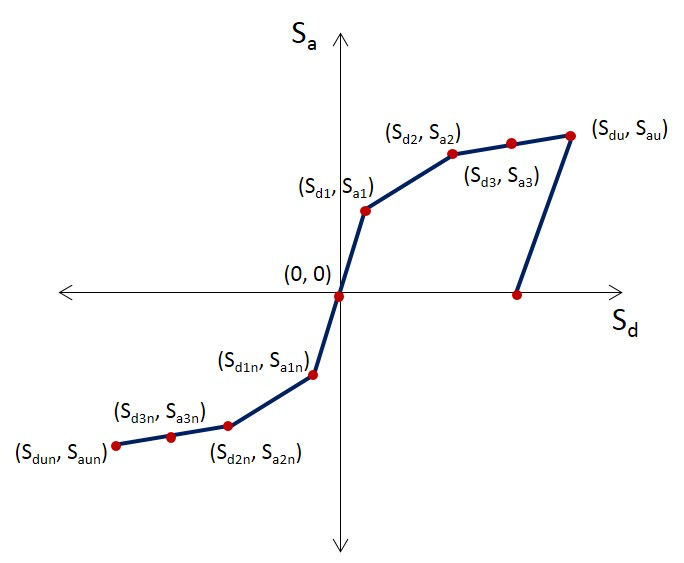
\includegraphics[width=9cm]{Figures/backbone_curve.png}
  \caption{Representation of the capacity curve required to represent the structural capacity of the SDOF system.}
  \label{fig:backbone}
\end{figure}

Six relevant points should be defined in this curve. The first one corresponds to the origin, (0, 0). The next point, (Sdy, Say), corresponds to the yielding point of the structure, i.e. the point beyond which the structure no longer displays an elastic behaviour. The following two points are defined as any two intermediate points between the yield point and the ultimate point which can be used to represent particular structural properties, such as reduction of stifness due to collapse of infill pannels or softning behavior due to P-delta effects. The ultimate point (Sdu, Sau) corresponds to the point of maximum displacement of the structure. Finally, the last point (Sdu, 0) is just a control point to define the hysteretic model, in case degradation is considered in the analysis. For the purposes of the RMTK, the first five points must be provided as input. The nonlinear time history analysis are performed using the open-source software for structural analysis OpenSees \citep{ McKennaEtAl2000}. It is important to understand the GEM Foundation does not have authorization to distriute this tool, and therefore in order to use this methodology, users are expected to download OpenSEES (http://opensees.berkeley.edu/), and allocate it in the appropriate folder (\verb=vulnerability/derivation_fragility/NLTHA_on_SDOF=).\\

In order to use this methodology, it is necessary to load one or multiple capacity curves and a set of ground motion records, as explained in Section \ref{subsec:cap_curves} and \ref{subsec:gmrs}, respectively. Then, it is necessary to specify a damage model using the parameter \verb=damage_model= (see Section \ref{subsec:dmg_model}). The damping ratio must be defined using the parameter \verb=damping=, and if structural degradation should be considered in the analysis, it is necessary to set the parameter \verb=degradation= to \verb=True=. After importing the module \verb=NLTHA_on_SDOF=, it is possible to calculate the distribution of structures across the set of damage states for each ground motion record using the following command:

\begin{Verbatim}[frame=single, commandchars=\\\{\}, samepage=true]
PDM, Sds = NLTHA_on_SDOF.calculate_fragility(capacity_curves,gmrs,...
damage_model,damping)
\end{Verbatim}

Where \verb=PDM= (i.e. probability damage matrix) represents a matrix with the number of structures in each damage state per ground motion record, and \verb=Sds= (i.e. spectral displacements) represents a matrix with the maximum displacement (of the equivalent SDOF) of each structure per ground motion record. the variable PDM can then be used to calculate the mean fragility model as described in Section \ref{subsec:derive_fragility}.





	\section{Derivation of fragility and vulnerability functions}
	\label{sec:derive_fragility}
	This section explains how a probability damage matrix (\verb=PDM=) can be used to derive a fragility function (i.e. probability of exceedance a number of
damage states for a set of intensity measure levels), and then converted into a vulnerability function  (i.e. distribution of loss ratio for a set of intensity measure levels), using a consequence model (see Section \ref{subsec:cons_model}). Both of these models can be exported in the OpenQuake-engine format (\verb=nrml=), or following a \verb=csv= format. Additional intructions about the necessary input models and associated formats can be found on the OpenQuake-engine User Guide \citep{GEM2015}.\\


		\subsection{Derivation of fragility functions}
		\label{subsec:derive_fragility}
		These fragility functions can be used directly by the Scenario Damage or the Classicla PSHA-based Damage calculators of the OpenQuake-engine (\cite{SilvaEtAl2014a}; \cite{PaganiEtAl2014a}). \\

In order to use the results of the nonlinear static procedures (see Section \ref{sec:record-nsp}) for the derivation of a fragility model, there are a number of attributes that need to be specified. Each function must be related with a building class, which must be defined using the parameter \verb=taxonomy=. Additional information about the GEM building taxonomy can be found in \cite{BrzevEtAl2013}, and a tool to compile the GEM taxonomy can be found on the OpenQuake-platform (https://taxtweb.openquake.org/).\\

For what concerns the definition of the seismic input, it is necessary to establish the intensity measure type that should be considered using the variable \verb=IMT=. Currently, the Risk Modeller's Toolkit supports \verb=PGA=, \verb=PGV= and \verb=Sa=. If the latter intensity measure type is chosen, it is also necessary to establish the period of vibration (in seconds) using the variable \verb=T=, and the elastic damping using the variable \verb=damping=. Finally, the range of applicability of the fragility model should be defined using the \verb=minIML= and \verb=maxIML=.  \\

The results in the probability damage matrix (\verb=PDM=) are used to fit a lognormal cumulative function, with a logarithmic mean ($\mu$) and logarithmic standard deviation ($\sigma$). These two parameters are calculated using one of the two currently implemented statistical methods: least squares or the maximum likelihood. The former approach estimates a solution ($\mu$, $\sigma$) that minimizes the sum of the squares of the errors (i.e. difference between the prediction of the lognormal function and the data). The latter method leads to a solution that maximizes the likelihood function. A comprehensive description of the strengths and limitations of these methodologies can be found in \cite{LallemantEtAl2015}. The method that should be followed must be specified by setting the parameter \verb=regression_method= to \verb=least squares= or to \verb=maximum likelihood=.\\

The calculation of the fragility model also requires the set of ground motion records used in the analytical analyses (\verb=gmrs=), and the damage model utilized to allocated each structure into a damage state (\verb=damage_model=). A description of these two components have been provided in Section \ref{subsec:gmrs} and \ref{subsec:dmg_model}, respectively.\\

The function that calculates fragility models is contained in the module \verb=utils=. An example of this process is depicted below.

\begin{Verbatim}[frame=single, commandchars=\\\{\}, samepage=true]
IMT = 'Sa'
T = 0.3
regression_method = 'least squares'
taxonomy = 'RC'
minIML = 0.01
maxIML = 1
fragility_model = utils.calculate_mean_fragility(gmrs,PDM,T,damping,...
IMT,damage_model,regression_method)
\end{Verbatim}

Once the parameters ($\mu$, $\sigma$) of the fragility model have been calculated, it is possible to save these results using the function \verb=save_mean_fragility=. This feature can export the fragility model using the OpenQuake-engine format (\verb=nrml=), or following a \verb=csv= format. This indication should be defined using the variable \verb=output_type=. It is also possible to create a plot of the resulting model, using the function \verb=plot_fragility_model=. In order to use these functions, it is necessary to import the module \verb=utils=. This process is demonstrated below. 

\begin{Verbatim}[frame=single, commandchars=\\\{\}, samepage=true]
output_type = 'nrml'
utils.save_mean_fragility(taxonomy,fragility_model,minIML,maxIML,...
output_type)
utils.plot_fragility_model(fragility_model,minIML,maxIML)
\end{Verbatim}

A detailed description of the \verb=nrml= format can be found on the OpenQuake-engine manual \citep{GEM2015}. For what concerns the structure of the \verb=csv= format, an example is provided in Table \ref{table:ff_csv}. The first row contains the building \verb=taxonomy=, the intensity measure type (\verb=IMT=), the minimum and maximum intensity measure levels (\verb=minIML=, \verb=maxIML=). The second row comprises the titles of the information stored in each column: damage states; logarithmic mean; logarithmic standard deviation; mean; standard deviation; median and coefficient of variation. The remaining columns contain the results for each damage state.

\begin {table}[htb]
\caption{Example of a fragility model stored following a csv format.}
\label{table:ff_csv}
\begin{center}
  \begin{tabular}{ | c | c | c | c | c | c | c |}
  \hline
RC & Sa(0.3) & 0.01 & 1.0 &  &  &  \\ \hline
Damage state & log mean & log stddev & mean & stddev & median & cov \\ \hline
Slight & -2.67 & 0.28 & 0.07 & 0.02 & 0.07 & 0.29 \\ \hline
Moderate & -2.37 & 0.30 & 0.10 & 0.03 & 0.09 & 0.31 \\ \hline
Extensive & -0.26 & 0.86 & 1.12 & 1.16 & 0.77 & 1.04 \\ \hline
Collapse & 0.42 & 0.96 & 2.42 & 2.99 & 1.52 & 1.24 \\ \hline
  \end{tabular}
\end{center}
\end{table}

Finally, a folder containing a set of fragility functions for buildings of different typologies derived using the RMTK and saved using the CSV format can be used to create a fragility model for use in OpenQuake risk analyses. In order to use the function \verb=save_fragility_set_nrml=, it is necessary to import the module \verb=utils=. The path to the folder containing the individual CSV fragility files, and the name of the destination XML file are the required inputs for this function. Usage of this function is shown below:

\begin{Verbatim}[frame=single, commandchars=\\\{\}, samepage=true]
utils.save_fragility_set_nrml(folder, destination_file)
\end{Verbatim}

		\subsection{Derivation of vulnerability functions}
		\label{subsec:derive_vulnerability}
		These vulnerability functions can be used directly by the Scenario Risk, Classical PSHA-based Risk and Probabilistic Event-based Risk calculators of the OpenQuake-engine (\cite{SilvaEtAl2014a}; \cite{PaganiEtAl2014a}). \\

A vulnerability model can be derived directly from loss data (either analytically generated or based on past seismic events), or by combining a set of fragility functions with a consequence model (see Section \ref{subsec:cons_model}). In this process, the fractions of buildings in each damage state are multiplied by the associated damage ratio (from the consequence model), in order to obtain a distribution of loss ratio for each intensity measure type. Currently only the latter approach is implemented in the Risk Modellers Toolkit, though the former method will be included in a future release.\\

The location of the consequence model must be defined using the parameter \verb=cons_model_file=, and load it into the Risk Modellers Toolkit using the function \verb=read_consequence_model=. The intensity measure levels for which the distribution of loss ratio will be calculated must be defined using the variable \verb=imls=.\\

The Risk Modellers Toolkit allows the propagation of the uncertainty in the consequence model to the vulnerability function. Thus, instead of just providing a single loss ratio per intensity measure type, it is possible to define a probabilistic model (following a \verb=lognormal= or \verb=beta= functions) or a non-parametric model (i.e. probability mass function - \verb=PMF=). This model must be defined using the variable \verb= distribution_type=.\\

The derivation of the vulnerability function also requires the previously computed \verb=fragility_model=. The function that calculates this result is contained in the module \verb=utils=. An example of this process is depicted below.

\begin{Verbatim}[frame=single, commandchars=\\\{\}, samepage=true]
cons_model_file = '../../../../../../rmtk_data/cons_model.csv'
cons_model = utils.read_consequence_model(cons_model_file)
imls = [0.1,0.2,0.3,0.4,0.5,0.6,0.8,0.9,1.0]
distribution_type = 'PMF'
vul_model = utils.convert_fragility_vulnerability(fragility_model,...
cons_model,imls,type_distribution)
\end{Verbatim}

The resulting vulnerability function can be saved using the function \verb=save_vulnerability=. This feature can export the vulnerability function using the OpenQuake-engine format (\verb=nrml=), or following a \verb=csv= format. Similarly to what was described for the fragility models, this indication should be provided using the variable \verb=output_type=. It is also possible to plot vulnerability functions, using the function \verb=plot_vulnerability_model=. In order to use these functions, it is necessary to import the module \verb=utils=. This process is demonstrated below.

\begin{Verbatim}[frame=single, commandchars=\\\{\}, samepage=true]
output_type = 'nrml'
utils.save_vulnerability(taxonomy,vulnerability_model,output_type)
utils.plot_vulnerability_model(vulnerability_model)
\end{Verbatim}

A detailed description of the \verb=nrml= format for vulnerability functions can be found on the OpenQuake-engine manual \citep{GEM2015}. For what concerns the structure of the \verb=csv= file, this format varies depending on how the uncertainty is being defined: parametric (lognormal or beta) or non-parametric (probability mass function). For the former case, an example is provided in Table \ref{table:vf_cont_csv}. The first row contains the building \verb=taxonomy=, the intensity measure type (\verb=IMT=), and the type of probabilistic model used to represent the uncertainty. The second row comprises the list of the intensity measure levels, and the means and associated coefficients of variation are provided in the third and forth row, respectively.

\begin {table}[htb]
\caption{Example of a vulnerability model with a parametric uncertainty modelling.}
\label{table:vf_cont_csv}
\begin{center}
  \begin{tabular}{ | c | c | c | c | c | c | c | c | c | c |}
  \hline
RC & Sa(0.3) & lognormal &  &  &  &  &  &  & \\ \hline
imls & 0.10 & 0.20 & 0.30 & 0.40 & 0.50 & 0.60 & 0.80 & 0.90 & 1.00\\ \hline
mean & 0.00 & 0.02 & 0.05 & 0.08 & 0.12 & 0.17 & 0.25 & 0.29 & 0.33\\ \hline
cov & 0.36 & 0.23 & 0.18 & 0.13 & 0.07 & 0.04 & 0.02 & 0.02 & 0.00\\ \hline
  \end{tabular}
\end{center}
\end{table}

For what concerns the \verb=csv= format for vulnerability functions using the non-parametric approach, an example can be found in Table \ref{table:vf_pmf_csv}. The first two rows are similar to the previous case, and the remaining columns contain the probability of having a given loss ratio, conditional on an intensity measure level.

\begin {table}[htb]
\caption{Example of a vulnerability model with a non-parametric uncertainty modelling.}
\label{table:vf_pmf_csv}
\begin{center}
  \begin{tabular}{ | c | c | c | c | c | c | c | c | c | c |}
  \hline
RC & Sa(0.3) & PMF &  &  &  &  &  &  & \\ \hline
imls & 0.10 & 0.20 & 0.30 & 0.40 & 0.50 & 0.60 & 0.80 & 0.90 & 1.00\\ \hline
loss ratio &  \multicolumn{9}{| c |}{probabilities} \\ \hline
0.00 & 0.80 & 0.15 & 0.00 & 0.00 & 0.00 & 0.00 & 0.00 & 0.00 & 0.00\\ \hline
0.11 & 0.20 & 0.60 & 0.30 & 0.00 & 0.00 & 0.00 & 0.00 & 0.00 & 0.00\\ \hline
0.22 & 0.00 & 0.25 & 0.60 & 0.40 & 0.00 & 0.00 & 0.00 & 0.00 & 0.00\\ \hline
0.33 & 0.00 & 0.00 & 0.10 & 0.50 & 0.20 & 0.00 & 0.00 & 0.00 & 0.00\\ \hline
0.44 & 0.00 & 0.00 & 0.00 & 0.10 & 0.70 & 0.10 & 0.00 & 0.00 & 0.00\\ \hline
0.56 & 0.00 & 0.00 & 0.00 & 0.00 & 0.10 & 0.50 & 0.10 & 0.00 & 0.00\\ \hline
0.67 & 0.00 & 0.00 & 0.00 & 0.00 & 0.00 & 0.35 & 0.30 & 0.00 & 0.00\\ \hline
0.78 & 0.00 & 0.00 & 0.00 & 0.00 & 0.00 & 0.05 & 0.50 & 0.10 & 0.00\\ \hline
0.89 & 0.00 & 0.00 & 0.00 & 0.00 & 0.00 & 0.00 & 0.10 & 0.70 & 0.00\\ \hline
1.00 & 0.00 & 0.00 & 0.00 & 0.00 & 0.00 & 0.00 & 0.00 & 0.20 & 1.00\\ \hline
  \end{tabular}
\end{center}
\end{table}

Finally, a folder containing a set of vulnerability functions for buildings of different typologies derived using the RMTK and saved using the CSV format can be used to create a vulnerability model for use in OpenQuake risk analyses. In order to use the function \verb=save_vulnerability_set_nrml=, it is necessary to import the module \verb=utils=. The path to the folder containing the individual CSV vulnerability files, and the name of the destination XML file are the required inputs for this function. Usage of this function is shown below:

\begin{Verbatim}[frame=single, commandchars=\\\{\}, samepage=true]
utils.save_vulnerability_set_nrml(folder, destination_file)
\end{Verbatim}

%----------------------------------------------------------------------------------------
%  APPENDICES
%----------------------------------------------------------------------------------------
\part*{Appendices}
\appendix
\chapter{The 10 Minute Guide to Python}
\label{chap:python_guide}
The RMTK is intended to be used by scientists and engineers without the necessity of having an existing knowledge of Python. It is hoped that the examples contained in this manual should provide enough context to allow the user to understand how to use the tools for their own needs. In spite of this, however, an understanding of the fundamentals of the Python programming language can greatly enhance the user experience and permit the user to join together the tools in a workflow that best matches their needs.

The aim of this appendix is therefore to introduce some fundamentals of the Python programming language in order to help understand how, and why, the HMTK can be used in a specific manner. If the reader wishes to develop their knowledge of the Python programming language beyond the examples shown here, there is a considerable body of literature on the topic from both a scientific and developer perspective.

\section{Basic Data Types}

Fundamental to the use of the HMTK is an understanding of the basic data types Python recognises:


\subsection{Scalar Parameters}

\begin{itemize}
\item \textbf{float} A floating point (decimal) number. If the user wishes to enter in a floating point value then a decimal point must be included, even if the number is rounded to an integer.

\begin{python}[frame=single]
>> a = 3.5
>> print a, type(a)
3.5 <type 'float'>
\end{python}

\item \textbf{integer} An integer number. If the decimal point is omitted for a floating point number the number will be considered an integer

\begin{python}[frame=single]
>> b = 3
>> print b, type(b)
3 <type 'int'>
\end{python}

The functions \verb=float()= and \verb=int()= can convert an integer to a float and vice-versa. Note that taking \verb=int()= of a fraction will round the fraction down to the nearest integer

\begin{python}[frame=single]
>> float(b)
3
>> int(a)
3
\end{python}

\item \textbf{string} A text string (technically a ``list'' of text characters). The string is indicated by the quotation marks ''something'' or 'something else'

\begin{python}[frame=single]
>> c = "apples"
>> print c, type(c)
apples <type 'str'>
\end{python}

\item \textbf{bool} For logical operations python can recognise a variable with a boolean data type (\verb=True= / \verb=False=).

\begin{python}[frame=single]
>> d = True
>> if d:
       print "y"
   else:
       print "n"
y
>> d = False
>> if d:
       print "y"
   else:
       print "n"
n
\end{python}

\emph{Care should be taken in Python as the value 0 and 0.0 are both recognised as False if applied to a logical operation. Similarly, booleans can be used in arithmetic where True and False take the values 1 and 0 respectively}

\begin{python}[frame=single]
>> d = 1.0
>> if d:
       print "y"
   else:
       print "n"
y
>> d = 0.0
>> if d:
       print "y"
   else:
       print "n"
n
\end{python}
\end{itemize}

\subsubsection{Scalar Arithmetic}

Scalars support basic mathematical operations (\# indicates a comment):

\begin{python}[frame=single]
>> a = 3.0
>> b = 4.0
>> a + b # Addition
7.0
>> a * b # Multiplication
12.0
>> a - b # Subtraction
-1.0
>> a / b # Division
0.75
>> a ** b  # Exponentiation
81.0
# But integer behaviour can be different!
>> a = 3; b = 4
>> a / b
0
>> b / a
1
\end{python}

\subsection{Iterables}

Python can also define variables as lists, tuples and sets. These data types can form the basis for iterable operations. It should be noted that unlike other languages, such as Matlab or Fortran, Python iterable locations are zero-ordered (i.e. the first location in a list has an index value of 0, rather than 1). 

\begin{itemize}
\item \textbf{List} A simple list of objects, which have the same or different data types. Data in lists can be re-assigned or replaced
\begin{python}[frame=single]
>> a_list = [3.0, 4.0, 5.0]
>> print a_list
[3.0, 4.0, 5.0]
>> another_list = [3.0, "apples", False]
>> print another_list
[3.0, 'apples', False]
>> a_list[2] = -1.0
a_list = [3.0, 4.0, -1.0]
\end{python}

\item \textbf{Tuples} Collections of objects that can be iterated upon. As with lists, they can support mixed data types. However, objects in a tuple cannot be re-assigned or replaced.
\begin{python}[frame=single]
>> a_tuple = (3.0, "apples", False)
>> print a_tuple
(3.0, 'apples', False)
# Try re-assigning a value in a tuple
>> a_tuple[2] = -1.0
TypeError                Traceback (most recent call last)
<ipython-input-43-644687cfd23c> in <module>()
----> 1 a_tuple[2] = -1.0

TypeError: 'tuple' object does not support item assignment
\end{python}

\item \textbf{Range} A range is a convenient function to generate arithmetic progressions. They are called with a \verb=start=, a \verb=stop= and (optionally) a \verb=step= (which defaults to 1 if not specified)

\begin{python}[frame=single]
>> a = range(0, 5)
>> print a
[0, 1, 2, 3, 4]  # Note that the stop number is not 
                 # included in the set!  
>> b = range(0, 6, 2)
>> print b
[0, 2, 4]
\end{python}

\item \textbf{Sets} A set is a special case of an iterable in which the elements are unordered, but contains more enhanced mathematical set operations (such as intersection, union, difference, etc.)

\begin{python}[frame=single]
>> from sets import Set
>> x = Set([3.0, 4.0, 5.0, 8.0])
>> y = Set([4.0, 7.0])
>> x.union(y)
Set([3.0, 4.0, 5.0, 7.0, 8.0])
>> x.intersection(y)
Set([4.0])
>> x.difference(y)
Set([8.0, 3.0, 5.0]) # Notice the results are not ordered!
\end{python}
\end{itemize}

\subsubsection{Indexing}

For some iterables (including lists, sets and strings) Python allows for subsets of the iterable to be selected and returned as a new iterable. The selection of elements within the set is done according to the \verb=index= of the set. 

\begin{python}[frame=single]
>> x = range(0, 10)  # Create an iterable
>> print x
[0, 1, 2, 3, 4, 5, 6, 7, 8, 9]
>> print x[0] # Select the first element in the set
0             # recall that iterables are zero-ordered!
>> print x[-1] # Select the last element in the set
9
>> y = x[:] # Select all the elements in the set
>> print y
[0, 1, 2, 3, 4, 5, 6, 7, 8, 9]
>> y = x[:4]  # Select the first four element of the set
>> print y
[0, 1, 2, 3]
>> y = x[-3:] # Select the last three elements of the set
>> print y
[7, 8, 9]
>> y = x[4:7] # Select the 4th, 5th and 6th elements
>> print y
[4, 5, 6]
\end{python}

\subsection{Dictionaries}

Python is capable of storing multiple data types associated with a map of variable names inside a single object. This is called a ``Dictionary'', and works in a similar manner to a ``data structure'' in languages such as Matlab. Dictionaries are used frequently in the HMTK as ways of structuring inputs to functions that share a common behaviour but may take different numbers and types of parameters on input.

\begin{python}[frame=single]
>> earthquake = {"Name": "Parkfield",
                 "Year": 2004,
                 "Magnitude": 6.1,
                 "Recording Agencies" = ["USGS", "ISC"]}
# To call or view a particular element in a dictionary
>> print earthquake["Name"], earthquake["Magnitude"]
Parkfield 6.1
\end{python}

\subsection{Loops and Logicals}

Python's syntax for undertaking logical operations and iterable operations is relatively straightforward.

\subsubsection{Logical}

A simple logical branching structure can be defined as follows:

\begin{python}[frame=single]
>> a = 3.5
>> if a <= 1.0:
       b = a + 2.0
   elif a > 2.0:
       b = a - 1.0
   else:
       b = a ** 2.0
>> print b
2.5
\end{python}

Boolean operations can are simply rendered as \verb=and=, \verb=or= and \verb=not=.
\begin{python}[frame=single]
>> a = 3.5
>> if (a <= 1.0) or (a > 3.0):
       b = a - 1.0
   else:
       b = a ** 2.0
>> print b
2.5
\end{python}

\subsubsection{Looping}

There are several ways to apply looping in python. For simple mathematical operations, the simplest way is to make use of the \textbf{range} function:

\begin{python}[frame=single]
>> for i in range(0, 5):
       print i, i ** 2
0  0
1  1
2  4
3  9
4  16
\end{python}

The same could be achieved using the \verb=while= function (though possibly this approach is far less desirable depending on the circumstance):

\begin{python}[frame=single]
>> i = 0
>> while i < 5:
       print i, i ** 2
       i += 1
0  0
1  1
2  4
3  9
4  16
\end{python}

A \verb=for= loop can be applied to any iterable:

\begin{python}[frame=single]
>> fruit_data = ["apples", "oranges", "bananas", "lemons", 
                 "cherries"]
>> i = 0
>> for fruit in fruit_data:
       print i, fruit
       i += 1
0  apples
1  oranges
2  bananas
3  lemons
4  cherries 
\end{python}

The same results can be generated, arguably more cleanly, by making use of the \verb=enumerate= function:

\begin{python}[frame=single]
>> fruit_data = ["apples", "oranges", "bananas", "lemons", 
                 "cherries"]
>> for i, fruit in enumerate(fruit_data):
       print i, fruit
0  apples
1  oranges
2  bananas
3  lemons
4  cherries 
\end{python}

As with many other programming languages, Python contains the statements \verb=break= to break out of a loop, and \verb=continue= to pass to the next iteration.

\begin{python}[frame=single]
>> i = 0
>> while i < 10:
       if i == 3:
           i += 1
           continue
       elif i == 5:
           break
       else:
           print i, i ** 2
       i += 1
0  0
1  1
2  4
4  16
\end{python}

\section{Functions}

Python easily supports the definition of functions. A simple example is shown below. \emph{Pay careful attention to indentation and syntax!}

\begin{python}[frame=single]
>> def a_simple_multiplier(a, b):
       """
       Documentation string - tells the reader the function 
       will multiply two numbers, and return the result and
       the square of the result
       """
       c = a * b
       return c, c ** 2.0

>> x = a_simple_multiplier(3.0, 4.0)
>> print x
(12.0, 144.0)
\end{python}

In the above example the function returns two outputs. If only one output is assigned then that output will take the form of a tuple, where the elements correspond to each of the two outputs. To assign directly, simply do the following:

\begin{python}[frame=single]
>> x, y = a_simple_multiplier(3.0, 4.0)
>> print x
12.0
>> print y
144.0
\end{python}

\section{Classes and Inheritance}

Python is one of many languages that is fully object-oriented, and the use (and terminology) of objects is prevalent throughout the HMTK and this manual. A full treatise on the topic of object oriented programming in Python is beyond the scope of this manual and the reader is referred to one of the many textbooks on Python for more examples

\subsection{Simple Classes}

A class is an object that can hold both attributes and methods. For example, imagine we wish to convert an earthquake magnitude from one scale to another; however, if the earthquake occurred after a user-defined year we wish to use a different formula. This could be done by a method, but we can also use a class:

\begin{python}[frame=single]
>> class MagnitudeConverter(object):
       """
       Class to convert magnitudes from one scale to another
       """
       def __init__(self, converter_year):
           """
           """
           self.converter_year = converter_year
       
       def convert(self, magnitude, year):
           """
           Converts the magnitude from one scale to another
           """
           if year < self.converter_year:
               converted_magnitude = -0.3 + 1.2 * magnitude
           else:
               converted_magnitude = 0.1 + 0.94 * magnitude
           return converted_magnitude
                  
>> converter1 = MagnitudeConverter(1990)
>> mag_1 = converter1.convert(5.0, 1987)
>> print mag_1
5.7
>> mag_2 = converter1.convert(5.0, 1994)
>> print mag_2
4.8
# Now change the conversion year
>> converter2 = MagnitudeConverter(1995)
>> mag_1 = converter2.convert(5.0, 1987)
>> print mag_1
5.7
>> mag_2 = converter2.convert(5.0, 1994)
>> print mag_2
5.7  
\end{python}

In this example the class holds both the attribute \verb=converter_year= and the method to convert the magnitude. The class is created (or ``instantiated'') with only the information regarding the cut-off year to use the different conversion formulae. Then the class has a method to convert a specific magnitude depending on its year.

\subsection{Inheritance}

Classes can be useful in many ways in programming. One such way is due to the property of inheritance. This allows for classes to be created that can inherit the attributes and methods of another class, but permit the user to add on new attributes and/or modify methods. 

In the following example we create a new magnitude converter, which may work in the same way as the \verb=MagnitudeConverter= class, but with different conversion methods.

\begin{python}[frame=single]
>> class NewMagnitudeConverter(MagnitudeConverter):
       """
       A magnitude converter using different conversion
       formulae
       """
       def convert(self, magnitude, year):
           """
           Converts the magnitude from one scale to another
           - differently!!!
           """
           if year < self.converter_year:
               converted_magnitude = -0.1 + 1.05 * magnitude
           else:
               converted_magnitude = 0.4 + 0.8 * magnitude
           return converted_magnitude
# Now compare converters
>> converter1 = MagnitudeConverter(1990)
>> converter2 = NewMagnitudeConverter(1990)
>> mag1 = converter1.convert(5.0, 1987)
>> print mag1
5.7
>> mag2 = converter2.convert(5.0, 1987)
>> print mag2
5.15
>> mag3 = converter1.convert(5.0, 1994)
>> print mag3
4.8
>> mag4 = converter2.convert(5.0, 1994)
>> print mag4
4.4    
\end{python}

\subsection{Abstraction}

Inspection of the HMTK code (\href{https://github.com/GEMScienceTools/hmtk}{https://github.com/GEMScienceTools/hmtk}) shows frequent usage of classes and inheritance. This is useful in our case if we wish to make available different methods for the same problem. In many cases the methods may have similar logic, or may provide the same types of outputs, but the specifics of the implementation may differ. Functions or attributes that are common to all methods can be placed in a ``Base Class'', permitting each implementation of a new method to inherit the ``Base Class'' and its functions/attributes/behaviour. The new method will simply modify those aspects of the base class that are required for the specific method in question. This allows functions to be used interchangeably, thus allowing for a "mapping" of data to specific methods. 

An example of abstraction is shown using our two magnitude converters shown previously. Imagine that a seismic recording network (named "XXX") has a model for converting from their locally recorded magnitude to a reference global scale (for the purposes of narrative, imagine that a change in recording procedures in 1990 results in a change of conversion model). A different recording network (named ``YYY'') has a different model for converting their local magnitude to a reference global scale (and we imagine they also changed their recording procedures, but they did so in 1994). We can create a mapping that would apply the correct conversion for each locally recorded magnitude in a short catalogue, provided we know the local magnitude, the year and the recording network.

\begin{python}[frame=single]
>> CONVERSION_MAP = {"XXX": MagnitudeConverter(1990),
                     "YYY": NewMagnitudeConverter(1994)}
>> earthquake_catalogue = [(5.0, "XXX", 1985),
                           (5.6, "YYY", 1992),
                           (4.8, "XXX", 1993),
                           (4.4, "YYY", 1997)]
>> for earthquake in earthquake_catalogue:
       converted_magnitude = \ # Line break for long lines!
           CONVERSION_MAP[earthquake[1]].convert(earthquake[0],
                                                 earthquake[2])
       print earthquake, converted_magnitude
(5.0, "XXX", 1985) 5.7
(5.6, "YYY", 1992) 5.78
(4.8, "XXX", 1993) 4.612
(4.4, "YYY", 1997) 3.92
\end{python}

So we have a simple magnitude homogenisor that applies the correct function depending on the network and year. It then becomes a very simple matter to add on new converters for new agencies; hence we have a ``toolkit'' of conversion functions!

\section{Numpy/Scipy}

Python has two powerful libraries for undertaking mathematical and scientific calculation, which are essential for the vast majority of scientific applications of Python: Numpy (for multi-dimensional array calculations) and Scipy (an extensive library of applications for maths, science and engineering). Both libraries are critical to both OpenQuake and the HMTK. Each package is so extensive that a comprehensive description requires a book in itself. Fortunately there is abundant documentation via the online help for Numpy \href{www.numpy.org}{www.numpy.org} and Scipy \href{www.scipy.org}{www.scipy.org}, so we do not need to go into detail here. 

The particular facet we focus upon is the way in which Numpy operates with respect to vector arithmatic. Users familiar with Matlab will recognise many similarities in the way the Numpy package undertakes array-based calculations. Likewise, as with Matlab, code that is well vectorised is signficantly faster and more efficient than the pure Python equivalent. 

The following shows how to undertake basic array arithmetic operations using the Numpy library

\begin{python}[frame=single]
>> import numpy as np
# Create two vectors of data, of equal length
>> x = np.array([3.0, 6.0, 12.0, 20.0])
>> y = np.array([1.0, 2.0, 3.0, 4.0])
# Basic arithmetic
>> x + y   # Addition (element-wise)
np.array([4.0, 8.0, 15.0, 24.0])
>> x + 2   # Addition of scalar
np.array([5.0, 8.0, 14.0, 22.0])
>> x * y   # Multiplication (element-wise)
np.array([3.0, 12.0, 36.0, 80.0])
>> x * 3.0   # Multiplication by scalar
np.array([9.0, 18.0, 36.0, 60.0])
>> x - y   # Subtraction (element-wise)
np.array([2.0, 4.0, 9.0, 16.0])
>> x - 1.0   # Subtraction of scalar
np.array([2.0, 5.0, 11.0, 19.0])
>> x / y   # Division (element-wise)
np.array([3.0, 3.0, 4.0, 5.0])
>> x / 2.0   # Division over scalar
np.array([1.5, 3.0, 6.0, 10.0])
>> x ** y    # Exponentiation (element-wise)
np.array([3.0, 36.0, 1728.0, 160000.0])
>> x ** 2.0   # Exponentiation (by scalar)
np.array([9.0, 36.0, 144.0, 400.0])
\end{python}

Numpy contains a vast set of mathematical functions that can be operated on a vector (e.g.):

\begin{python}[frame=single]
>> x = np.array([3.0, 6.0, 12.0, 20.0])
>> np.exp(x)
np.array([2.00855369e+01, 4.03428793e+02, 1.62754791e+05,
         4.85165195e+08])
# Trigonometry
>> theta = np.array([0., np.pi / 2.0, np.pi, 1.5 * np.pi])
>> np.sin(theta)
np.array([0.0000, 1.0000, 0.0000, -1.0000])
>> np.cos(theta)
np.array([1.0000, 0.0000, -1.0000, 0.0000])
\end{python}

Some of the most powerful functions of Numpy, however, come from its logical indexing:

\begin{python}[frame=single]
>> x = np.array([3.0, 5.0, 12.0, 21.0, 43.0])
>> idx = x >= 10.0   # Perform a logical operation
>> print idx
np.array([False, False, True, True, True])
>> x[idx]   # Return an array consisting of elements
            # for which the logical operation returned True
np.array([12.0, 21.0, 43.0])
\end{python}

Create, index and slice n-dimensional arrays:

\begin{python}[frame=single]
>> x = np.array([[3.0,  5.0, 12.0, 21.0, 43.0],
                 [2.0,  1.0,  4.0, 12.0, 30.0],
                 [1.0, -4.0, -2.1,  0.0, 92.0]])
>> np.shape(x)
(3, 5)
>> x[:, 0]
np.array([3.0, 2.0, 1.0])
>> x[1, :]
np.array([2.0, 1.0, 4.0, 12.0, 30.0])
>> x[:, [1, 4]]
np.array([[ 5.0, 43.0],
          [ 1.0, 30.0],
          [-4.0, 92.0]])
\end{python}

The reader is referred to the online documentation for the full set of functions!





%-------------------------------------------------------------------------------
%  BIBLIOGRAPHY
%-------------------------------------------------------------------------------

\chapter*{Bibliography}
\addcontentsline{toc}{chapter}{\textcolor{darkgray}{Bibliography}}
\section*{Books}
\printbibliography[heading=bibempty,type=book]
\section*{Articles}
\printbibliography[heading=bibempty,type=article]
\section*{Other Sources}
\printbibliography[heading=bibempty,nottype=book,nottype=article]
\cleardoublepage

%-------------------------------------------------------------------------------
%  INDEX & GLOSSARY
%-------------------------------------------------------------------------------

\printindex
\chapter*{Glossary}
\addcontentsline{toc}{chapter}{\textcolor{darkgray}{Glossary}}
\printglossary[type=acronym, title=List of Acronyms]
\printglossary[title=List of Terms]
\hfill \\ \thispagestyle{empty} \clearpage % ---------------- Final empty page -


\end{document}